\documentclass[tikz]{standalone}\usepackage[]{graphicx}\usepackage[]{color}
%% maxwidth is the original width if it is less than linewidth
%% otherwise use linewidth (to make sure the graphics do not exceed the margin)
\makeatletter
\def\maxwidth{ %
  \ifdim\Gin@nat@width>\linewidth
    \linewidth
  \else
    \Gin@nat@width
  \fi
}
\makeatother

\definecolor{fgcolor}{rgb}{0.345, 0.345, 0.345}
\newcommand{\hlnum}[1]{\textcolor[rgb]{0.686,0.059,0.569}{#1}}%
\newcommand{\hlstr}[1]{\textcolor[rgb]{0.192,0.494,0.8}{#1}}%
\newcommand{\hlcom}[1]{\textcolor[rgb]{0.678,0.584,0.686}{\textit{#1}}}%
\newcommand{\hlopt}[1]{\textcolor[rgb]{0,0,0}{#1}}%
\newcommand{\hlstd}[1]{\textcolor[rgb]{0.345,0.345,0.345}{#1}}%
\newcommand{\hlkwa}[1]{\textcolor[rgb]{0.161,0.373,0.58}{\textbf{#1}}}%
\newcommand{\hlkwb}[1]{\textcolor[rgb]{0.69,0.353,0.396}{#1}}%
\newcommand{\hlkwc}[1]{\textcolor[rgb]{0.333,0.667,0.333}{#1}}%
\newcommand{\hlkwd}[1]{\textcolor[rgb]{0.737,0.353,0.396}{\textbf{#1}}}%
\let\hlipl\hlkwb

\usepackage{framed}
\makeatletter
\newenvironment{kframe}{%
 \def\at@end@of@kframe{}%
 \ifinner\ifhmode%
  \def\at@end@of@kframe{\end{minipage}}%
  \begin{minipage}{\columnwidth}%
 \fi\fi%
 \def\FrameCommand##1{\hskip\@totalleftmargin \hskip-\fboxsep
 \colorbox{shadecolor}{##1}\hskip-\fboxsep
     % There is no \\@totalrightmargin, so:
     \hskip-\linewidth \hskip-\@totalleftmargin \hskip\columnwidth}%
 \MakeFramed {\advance\hsize-\width
   \@totalleftmargin\z@ \linewidth\hsize
   \@setminipage}}%
 {\par\unskip\endMakeFramed%
 \at@end@of@kframe}
\makeatother

\definecolor{shadecolor}{rgb}{.97, .97, .97}
\definecolor{messagecolor}{rgb}{0, 0, 0}
\definecolor{warningcolor}{rgb}{1, 0, 1}
\definecolor{errorcolor}{rgb}{1, 0, 0}
\newenvironment{knitrout}{}{} % an empty environment to be redefined in TeX

\usepackage{alltt}
\IfFileExists{upquote.sty}{\usepackage{upquote}}{}
\begin{document}

\begin{knitrout}
\definecolor{shadecolor}{rgb}{0.969, 0.969, 0.969}\color{fgcolor}\begin{kframe}


{\ttfamily\noindent\bfseries\color{errorcolor}{\#\# Error in check\_font\_path(regular, "{}regular"{}): font file not found for 'regular' type}}\end{kframe}
\end{knitrout}















\section{Fiscal challenges}



\begin{knitrout}
\definecolor{shadecolor}{rgb}{0.969, 0.969, 0.969}\color{fgcolor}
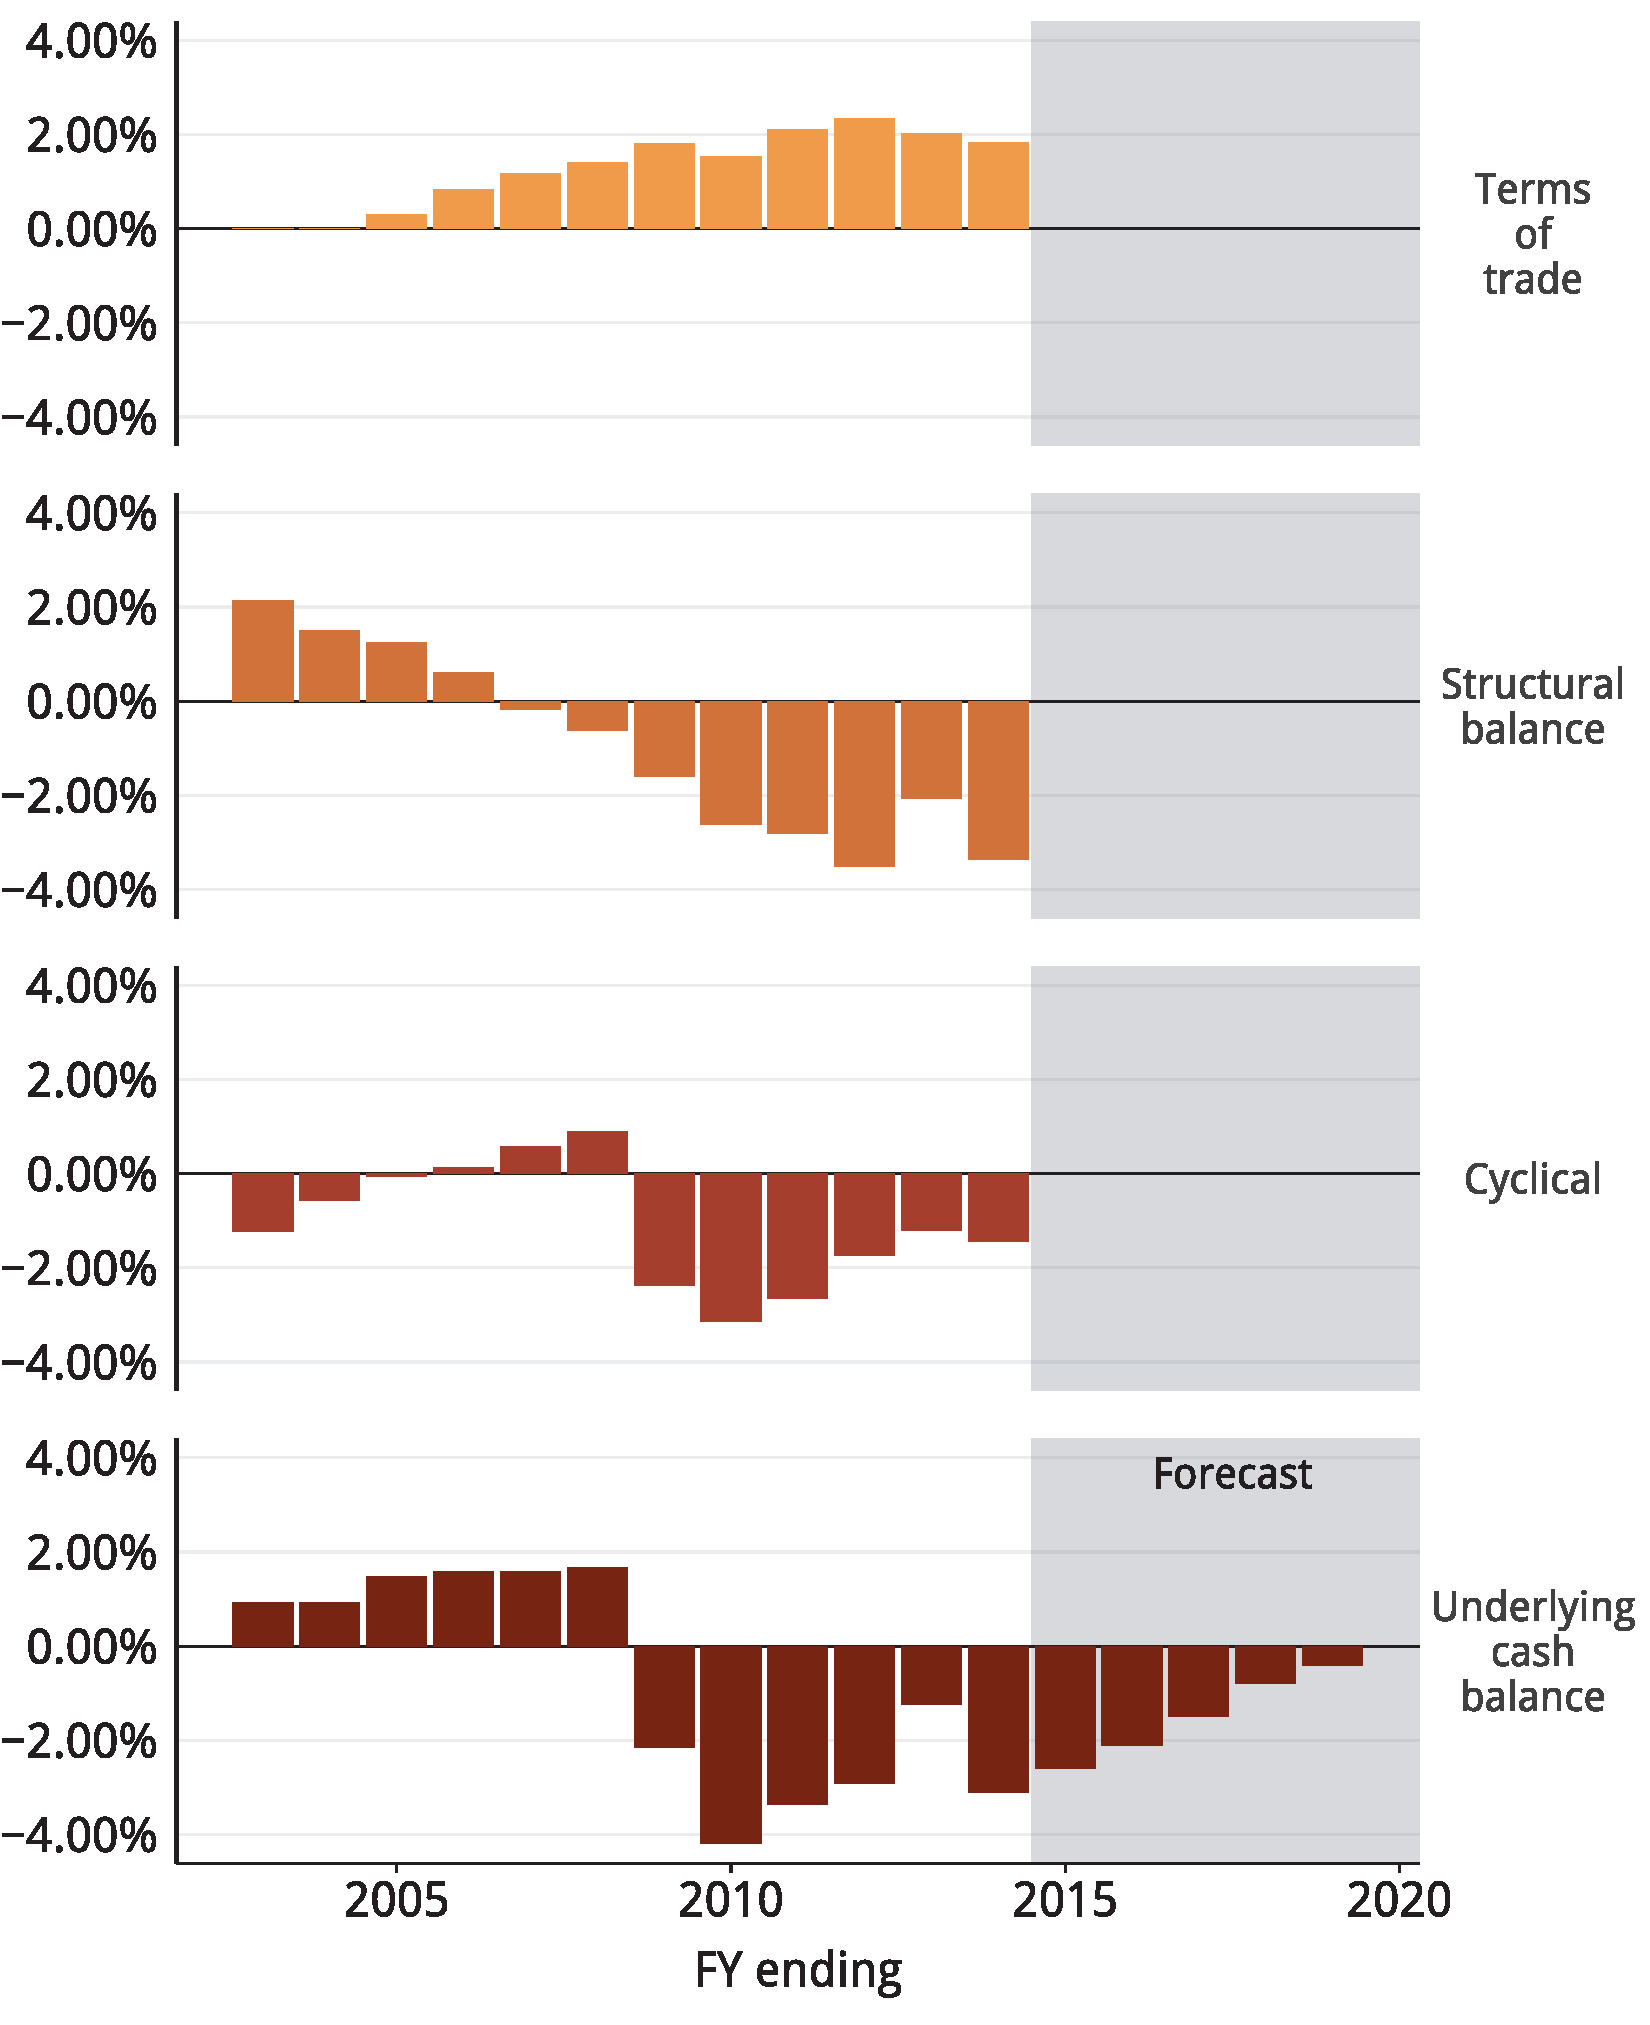
\includegraphics[width=11.000in,height=13.5in]{./b5-figure/FISCAL-b5-Figure1-1} 

\end{knitrout}

\begin{knitrout}
\definecolor{shadecolor}{rgb}{0.969, 0.969, 0.969}\color{fgcolor}
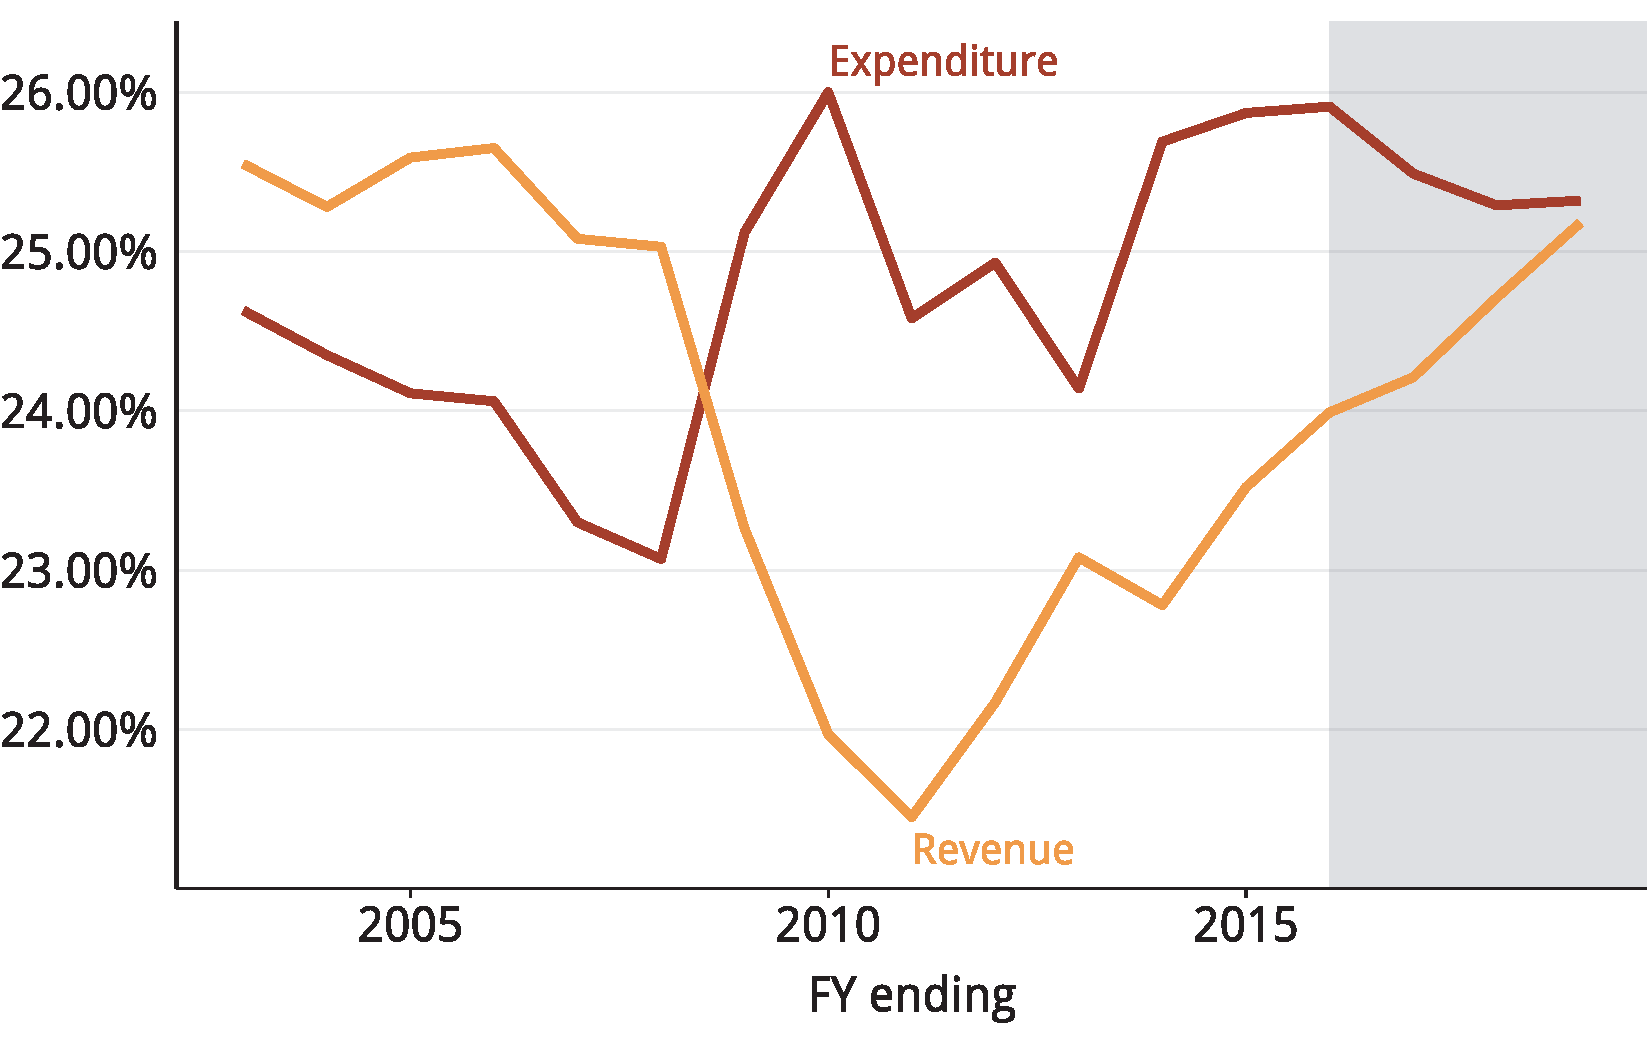
\includegraphics[width=11.000in,height=7.00in]{./b5-figure/FISCAL-Figure2-1} 

\end{knitrout}

\begin{knitrout}
\definecolor{shadecolor}{rgb}{0.969, 0.969, 0.969}\color{fgcolor}
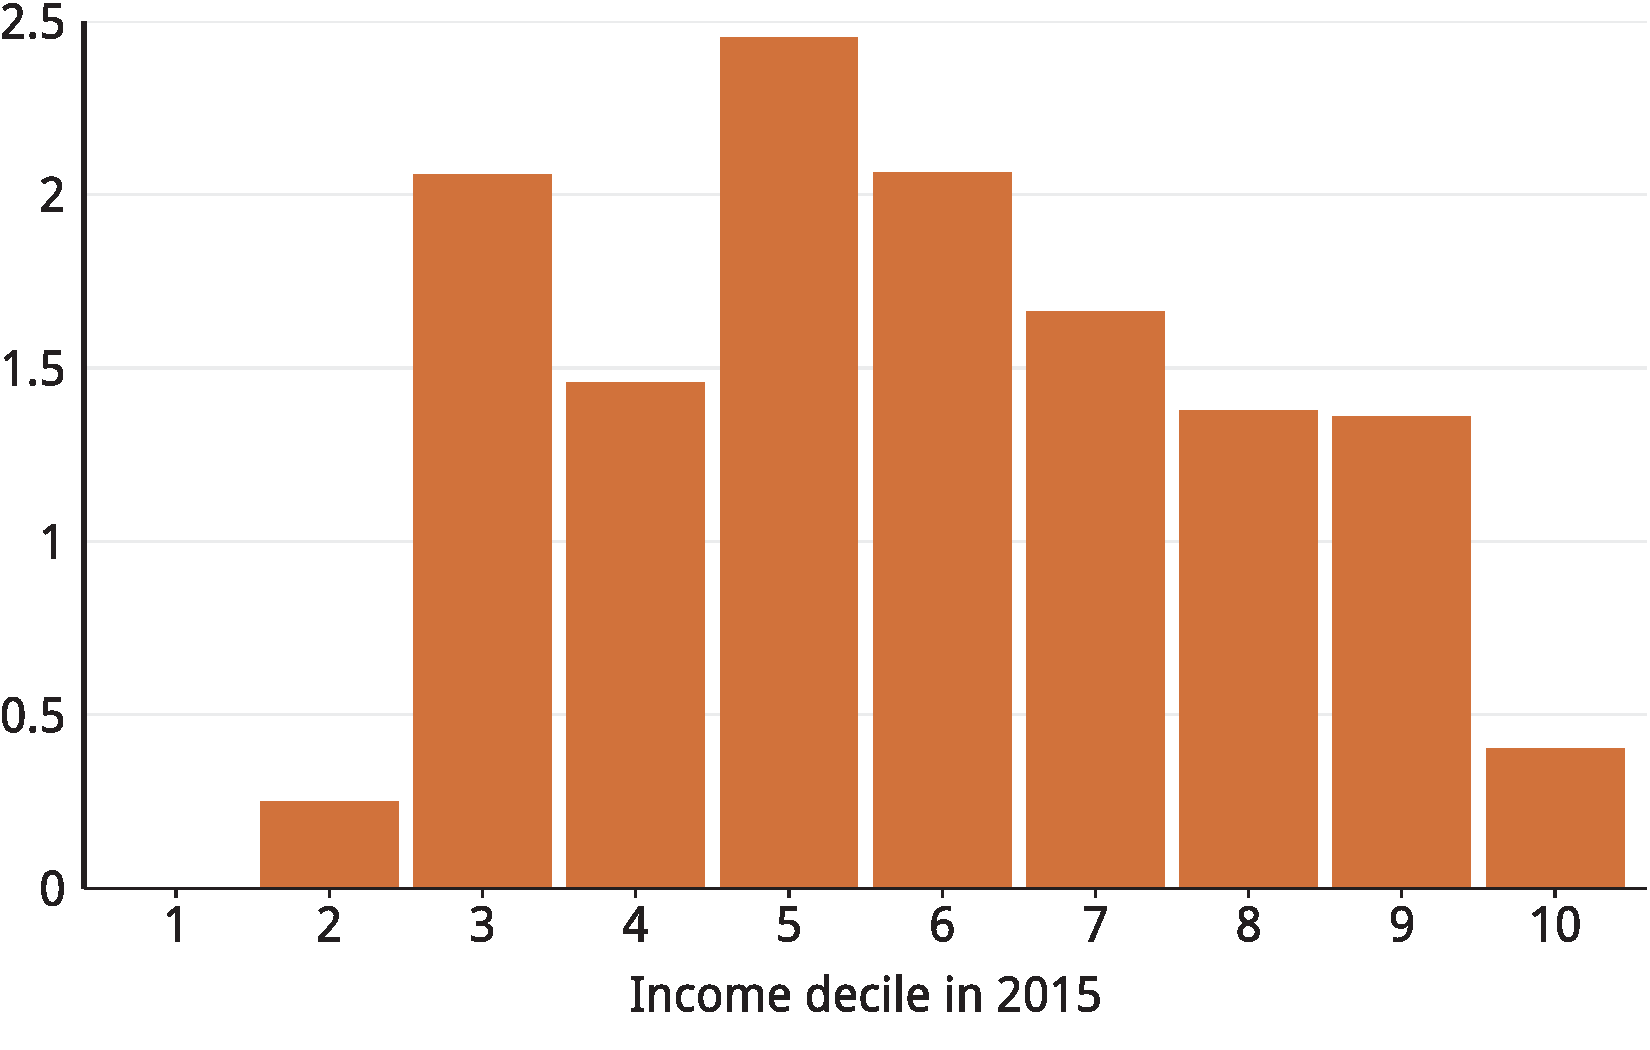
\includegraphics[width=11.000in,height=7.00in]{./b5-figure/FISCAL-Figure4-1} 

\end{knitrout}

\begin{knitrout}
\definecolor{shadecolor}{rgb}{0.969, 0.969, 0.969}\color{fgcolor}
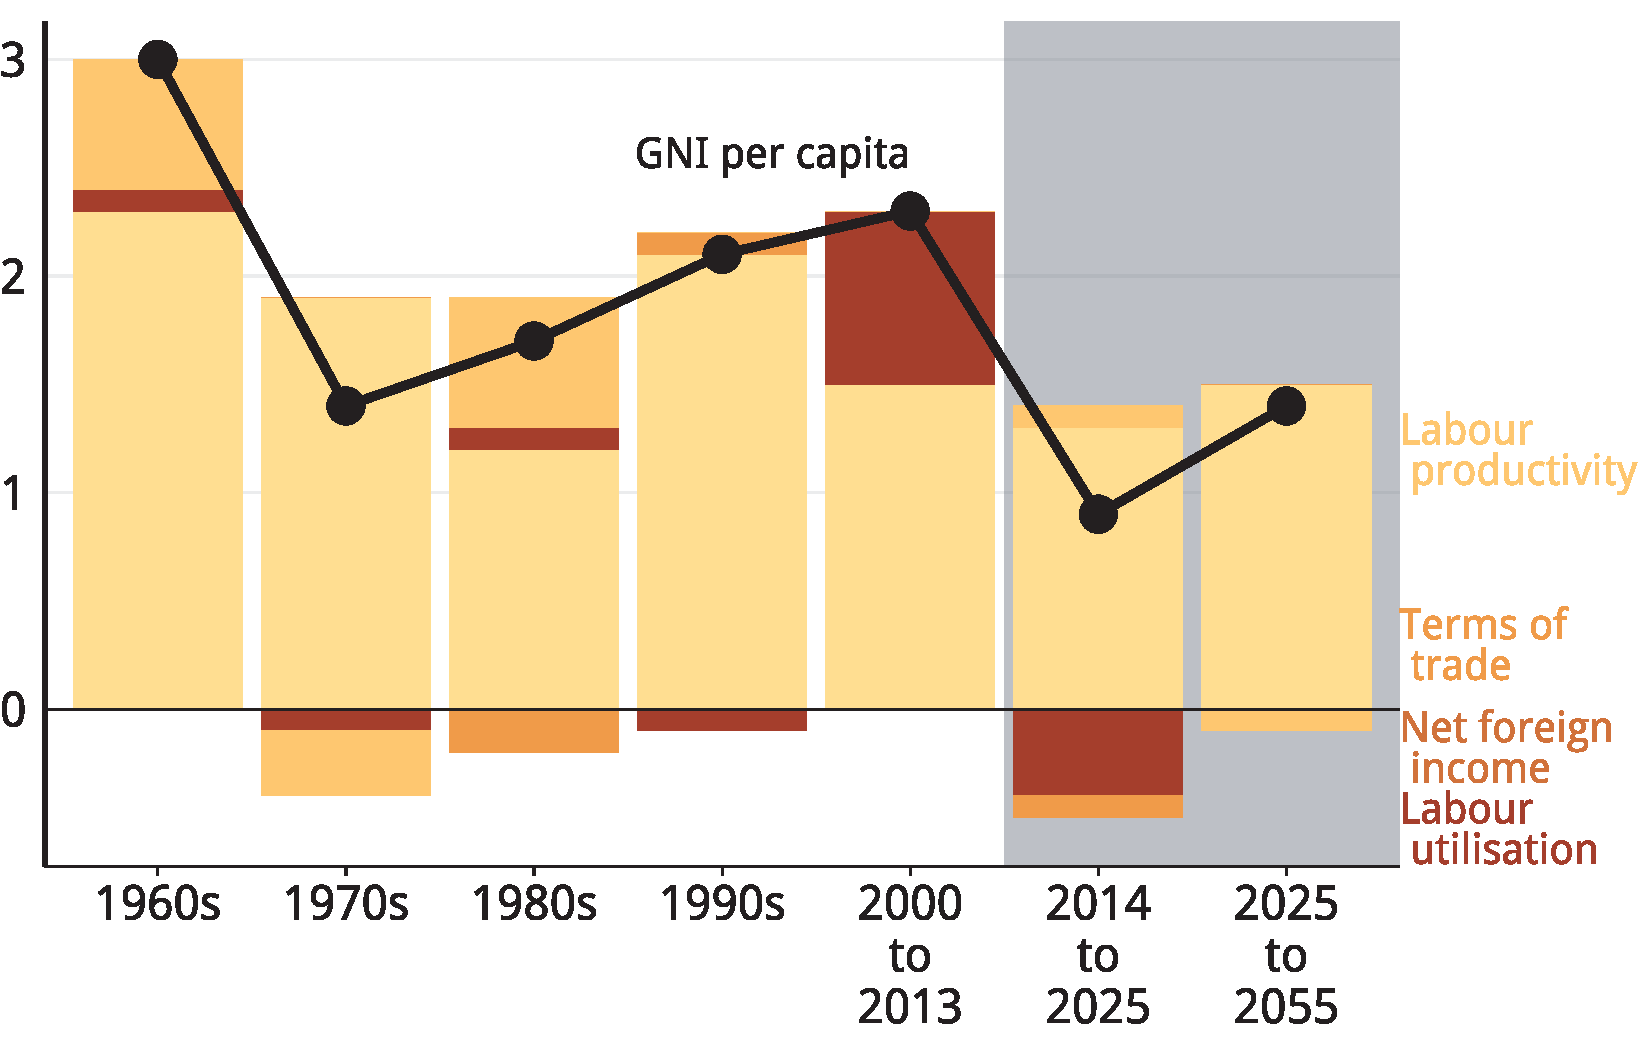
\includegraphics[width=11.000in,height=7.00in]{./b5-figure/FISCAL-Figure5-1} 

\end{knitrout}

\begin{knitrout}
\definecolor{shadecolor}{rgb}{0.969, 0.969, 0.969}\color{fgcolor}
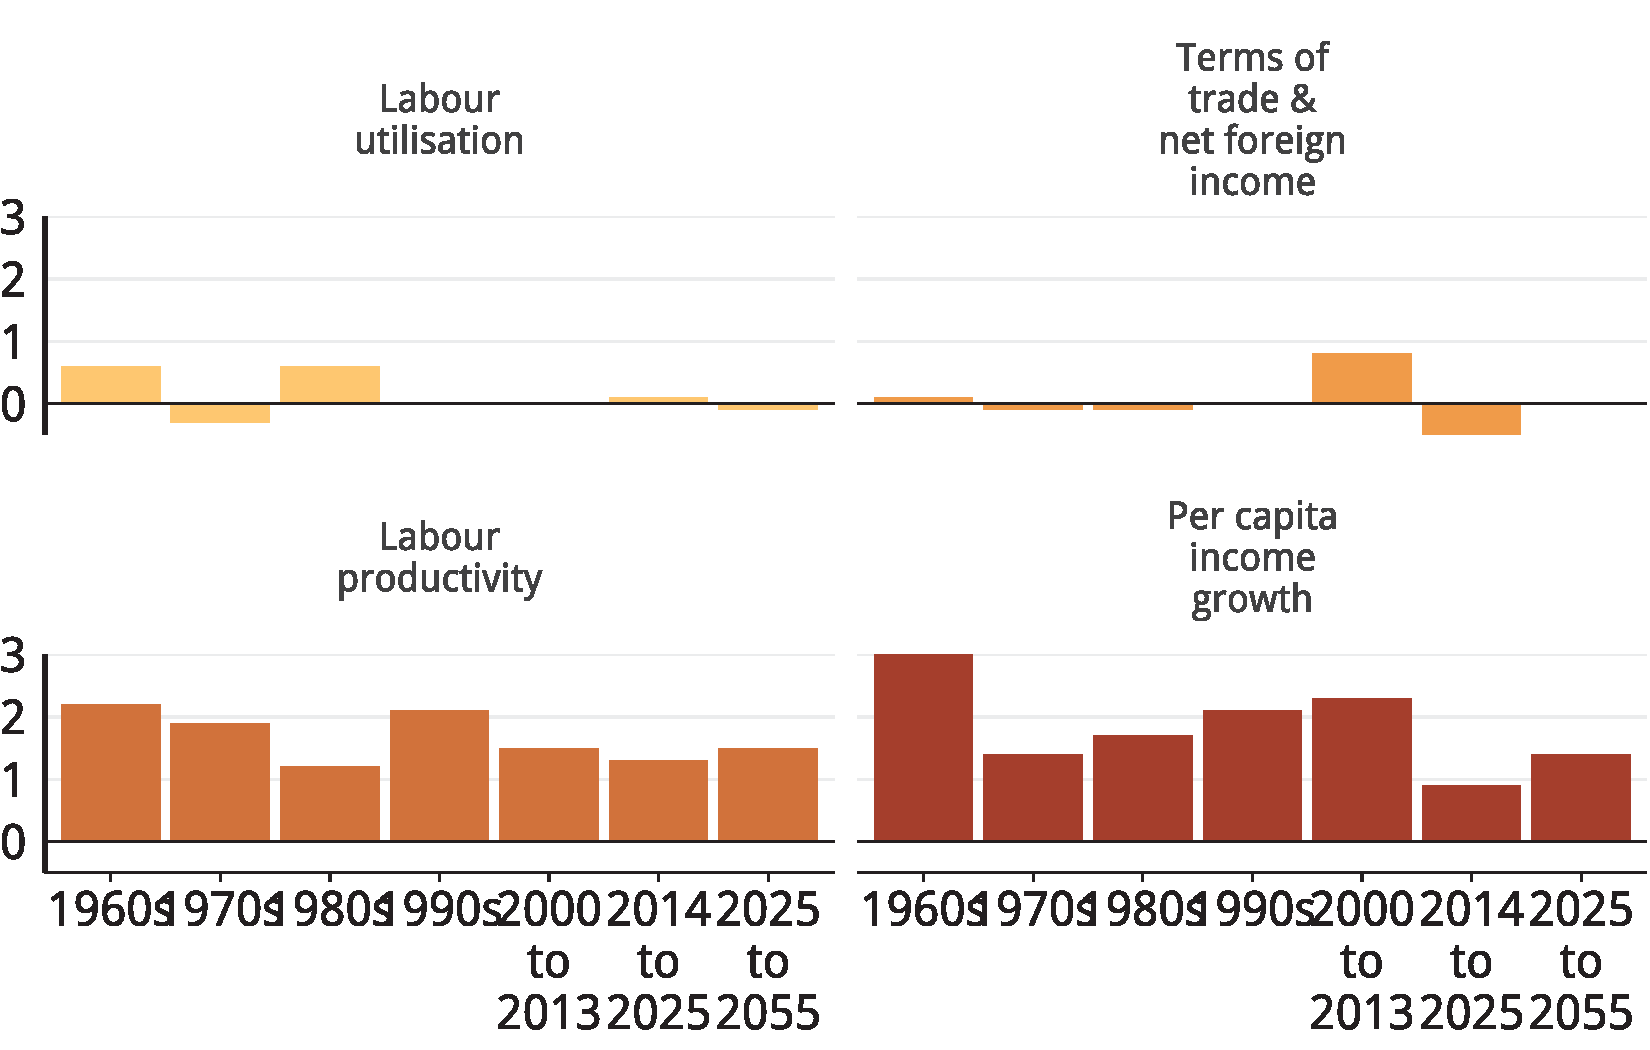
\includegraphics[width=11.000in,height=7.00in]{./b5-figure/FISCAL-Figure5-alt-1} 

\end{knitrout}

\begin{knitrout}
\definecolor{shadecolor}{rgb}{0.969, 0.969, 0.969}\color{fgcolor}
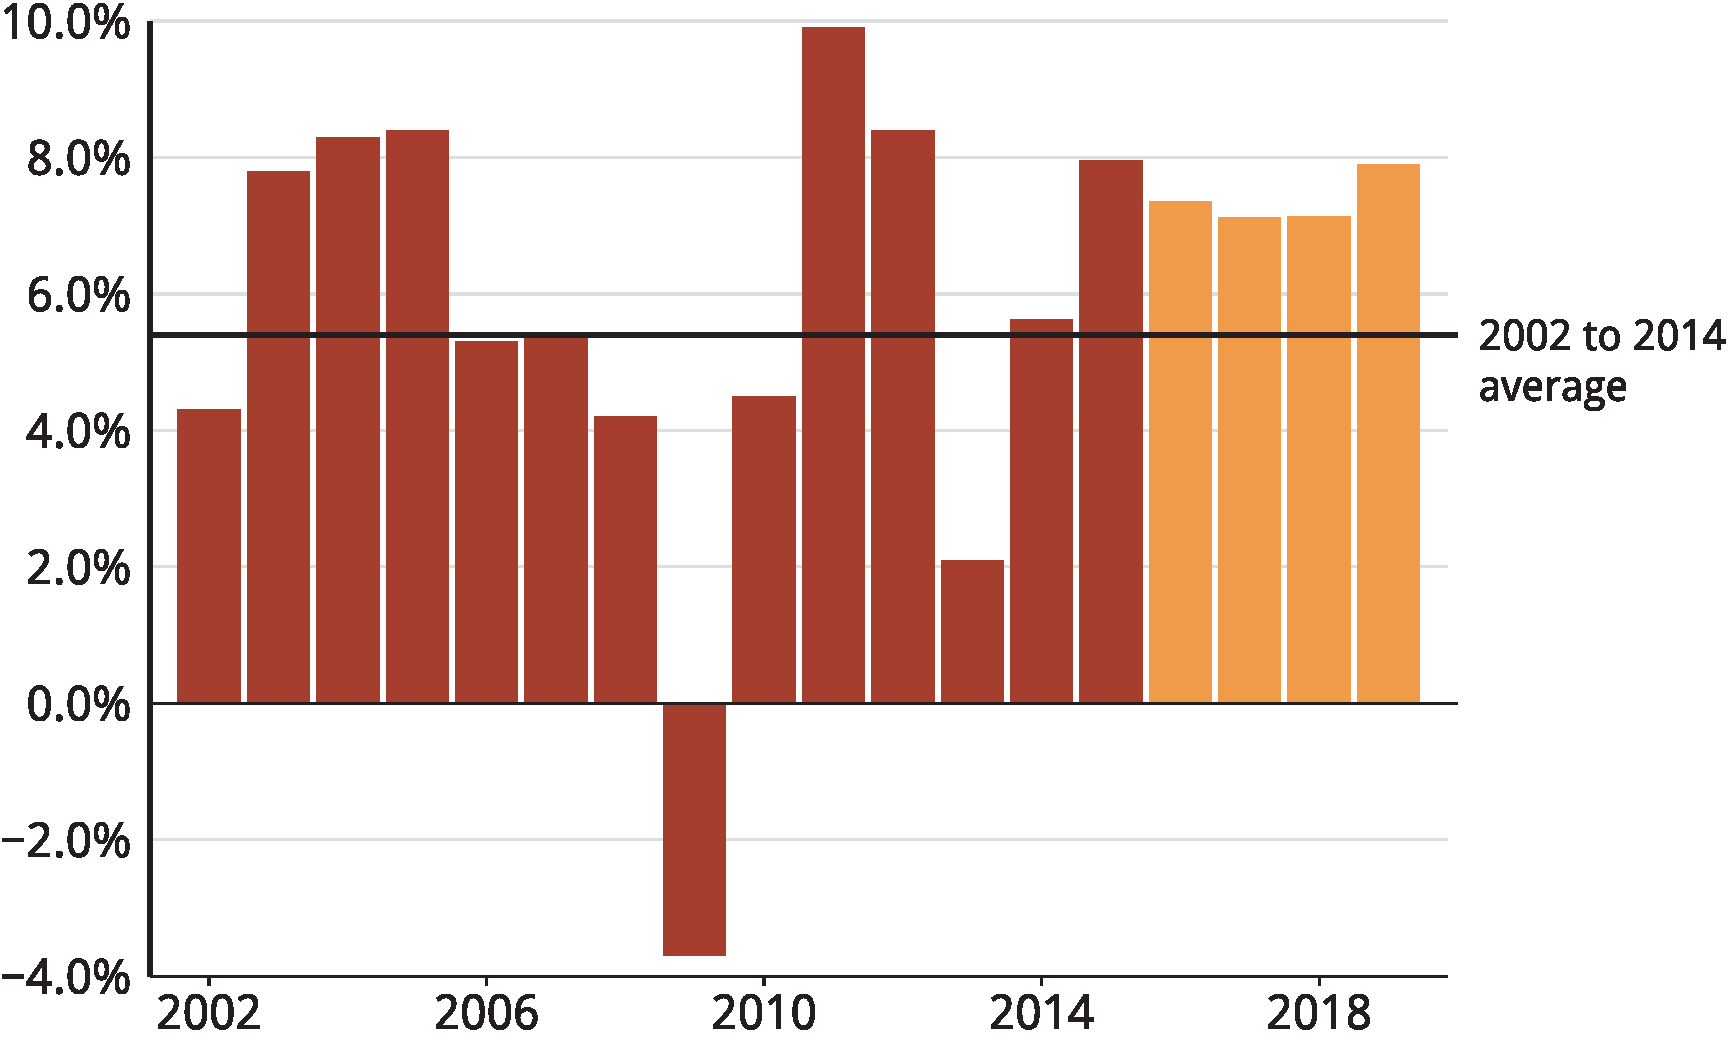
\includegraphics[width=11.55in,height=7.00in]{./b5-figure/FISCAL-Figure6-1} 

\end{knitrout}

\begin{knitrout}
\definecolor{shadecolor}{rgb}{0.969, 0.969, 0.969}\color{fgcolor}
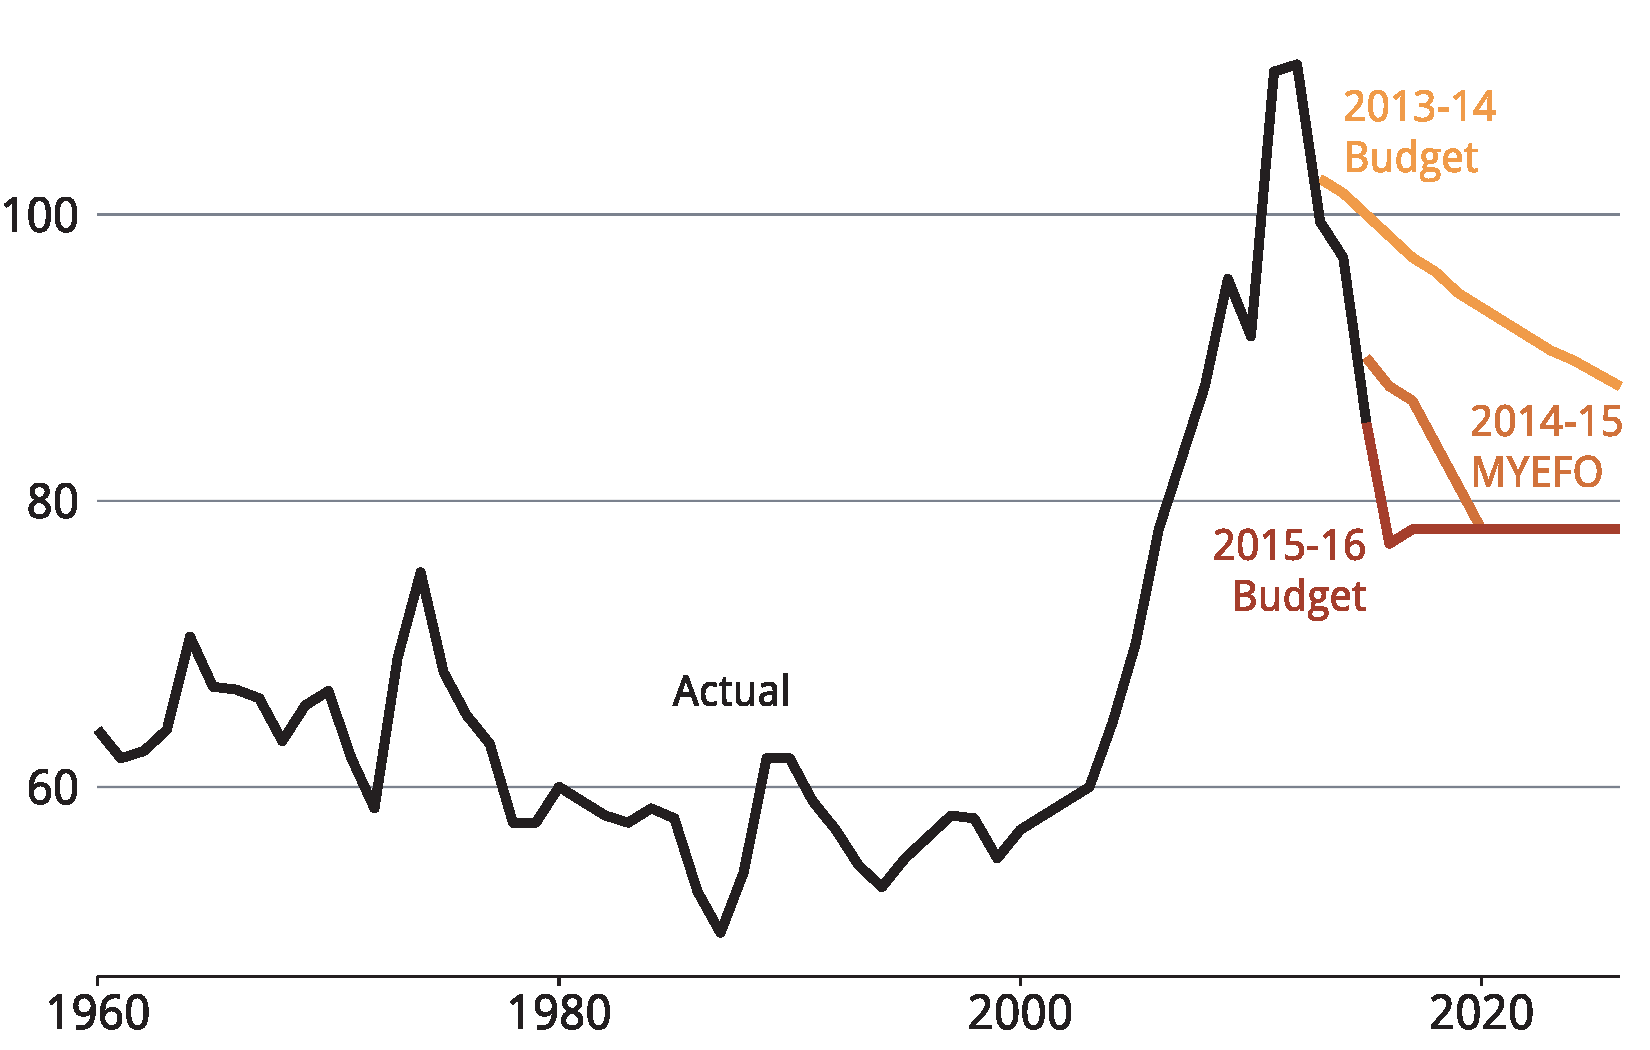
\includegraphics[width=11.000in,height=7.00in]{./b5-figure/FISCAL-Figure7-1} 

\end{knitrout}

\begin{knitrout}
\definecolor{shadecolor}{rgb}{0.969, 0.969, 0.969}\color{fgcolor}
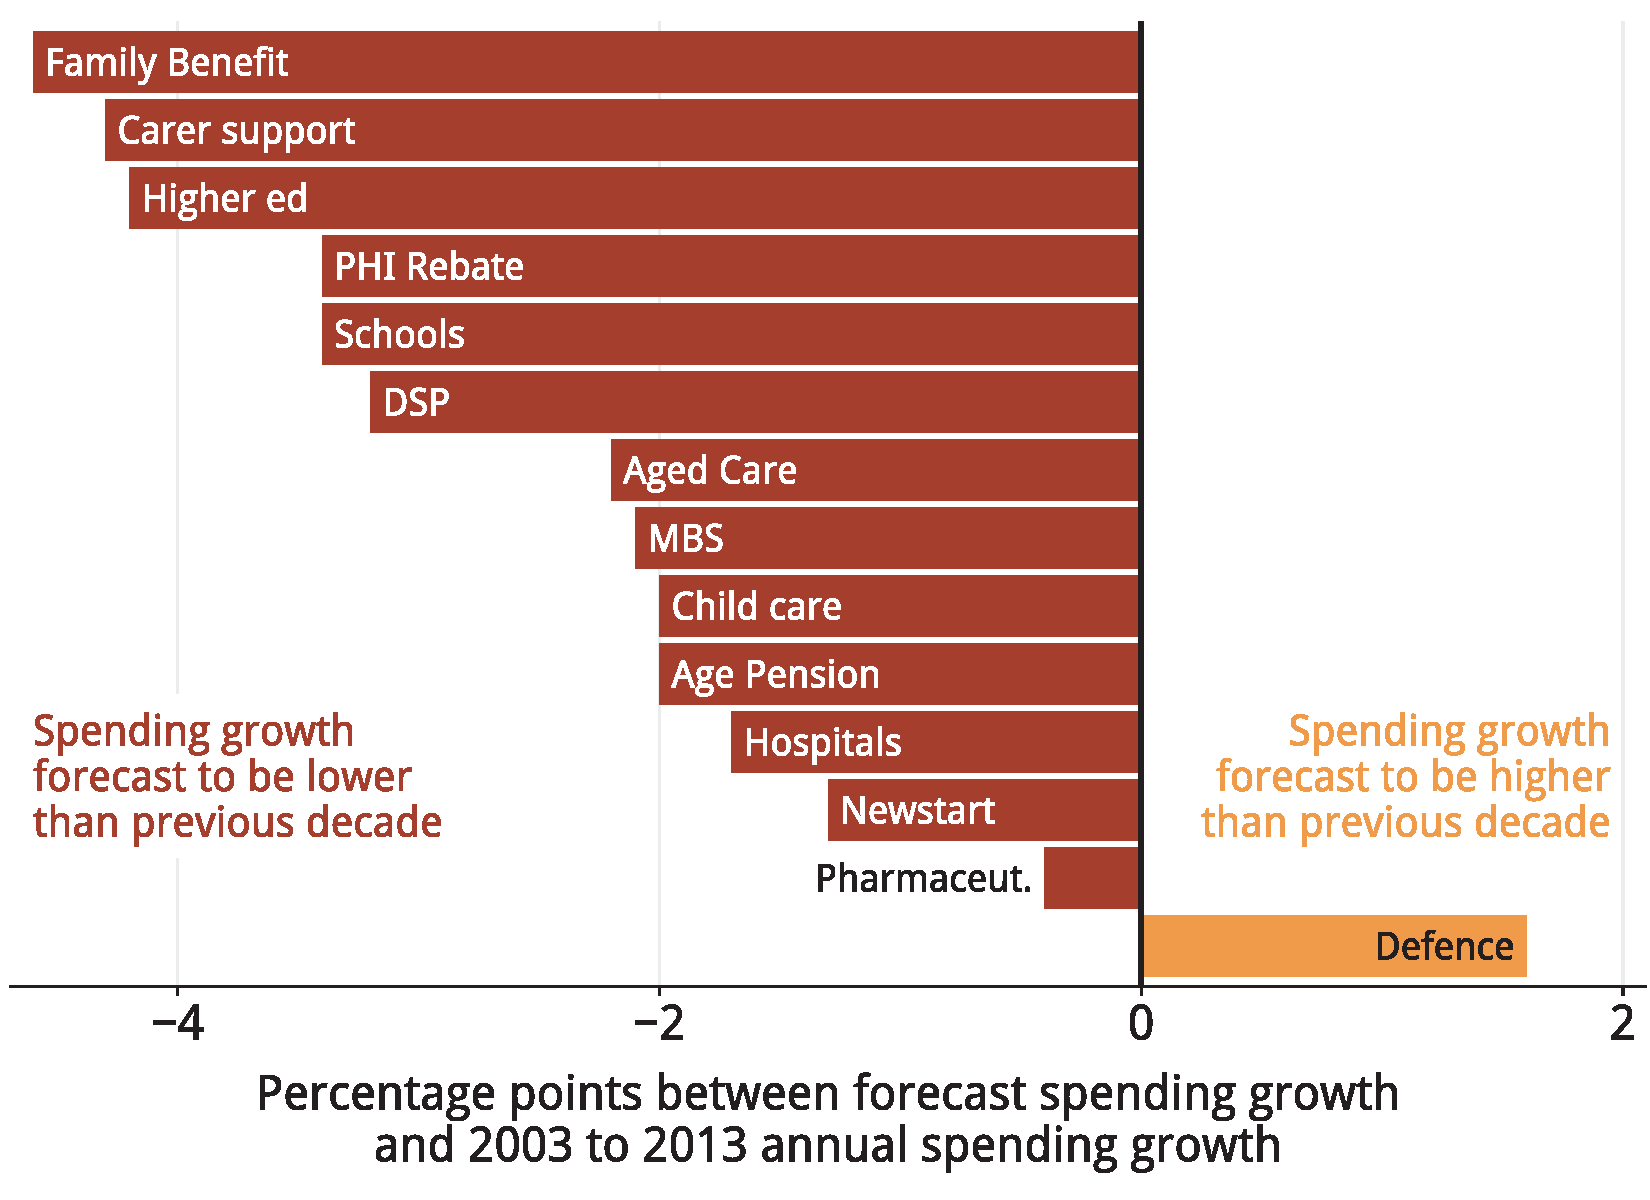
\includegraphics[width=11.000in,height=8in]{./b5-figure/FISCAL-Figure8-altered-1} 

\end{knitrout}

\clearpage
\begin{knitrout}
\definecolor{shadecolor}{rgb}{0.969, 0.969, 0.969}\color{fgcolor}
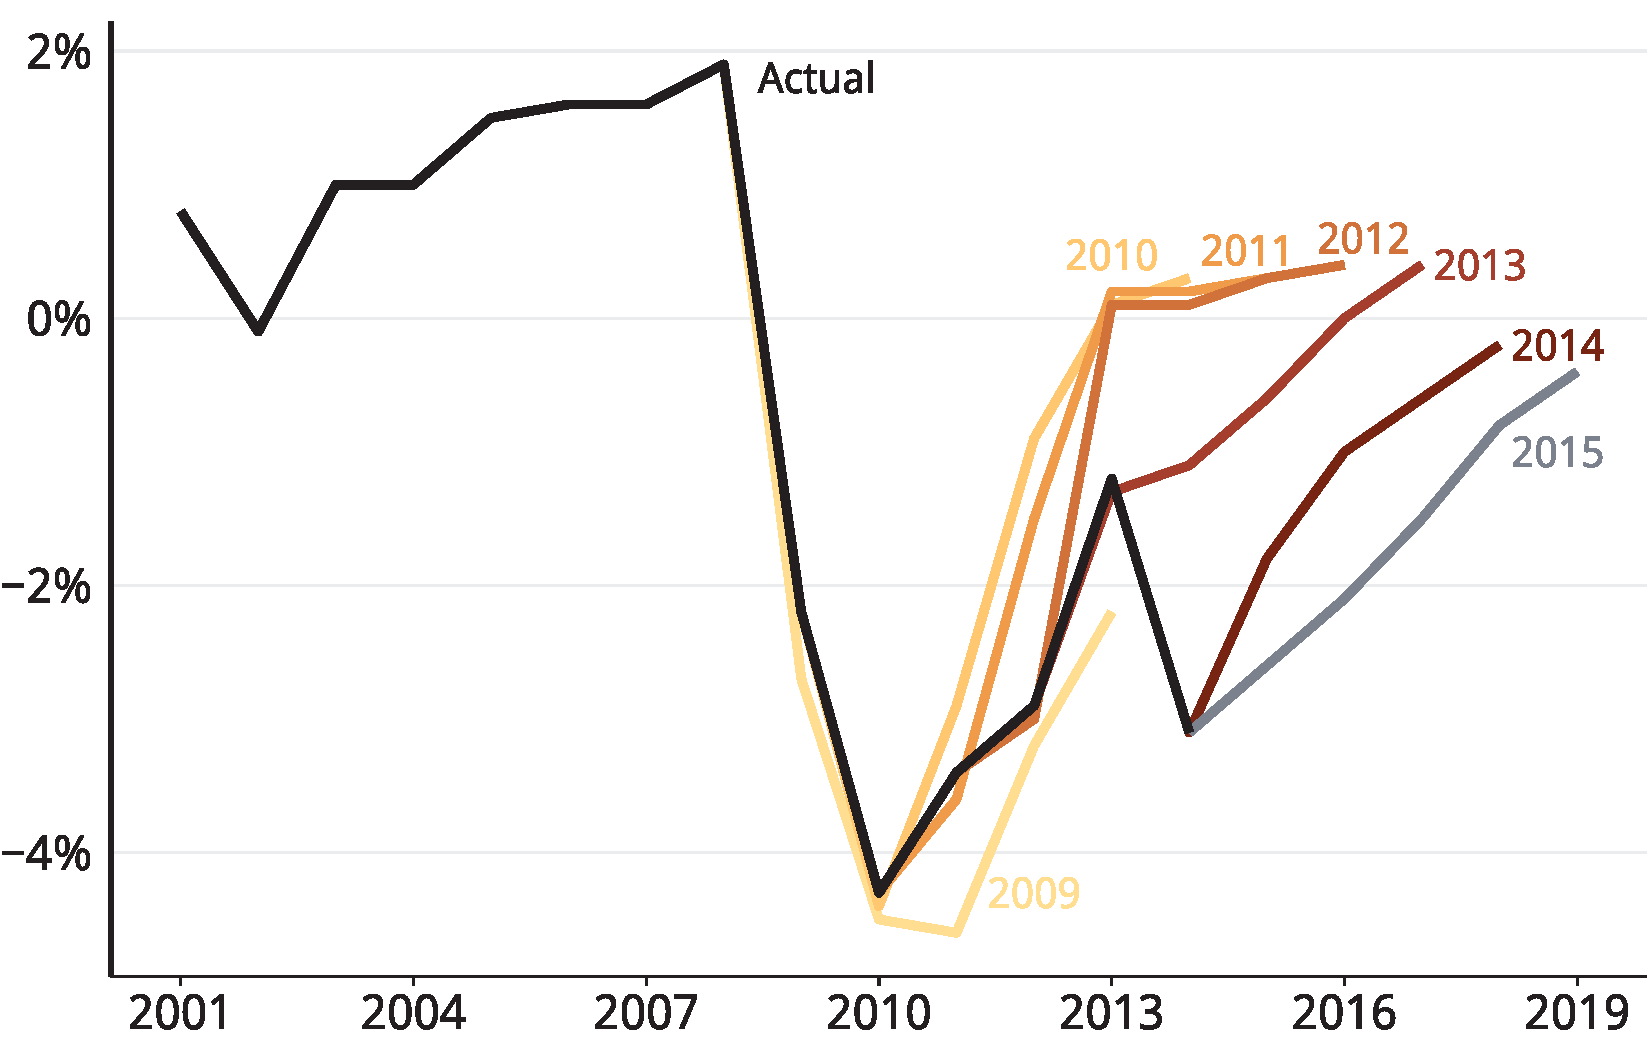
\includegraphics[width=11.000in,height=7.00in]{./b5-figure/FISCAL-Figure9a-1} 

\end{knitrout}
\clearpage

\begin{knitrout}
\definecolor{shadecolor}{rgb}{0.969, 0.969, 0.969}\color{fgcolor}\begin{kframe}


{\ttfamily\noindent\bfseries\color{errorcolor}{\#\# Error: `path` does not exist: './Fiscal-challenges/Figure10.xlsx'}}\end{kframe}
\end{knitrout}

\clearpage
\begin{knitrout}
\definecolor{shadecolor}{rgb}{0.969, 0.969, 0.969}\color{fgcolor}
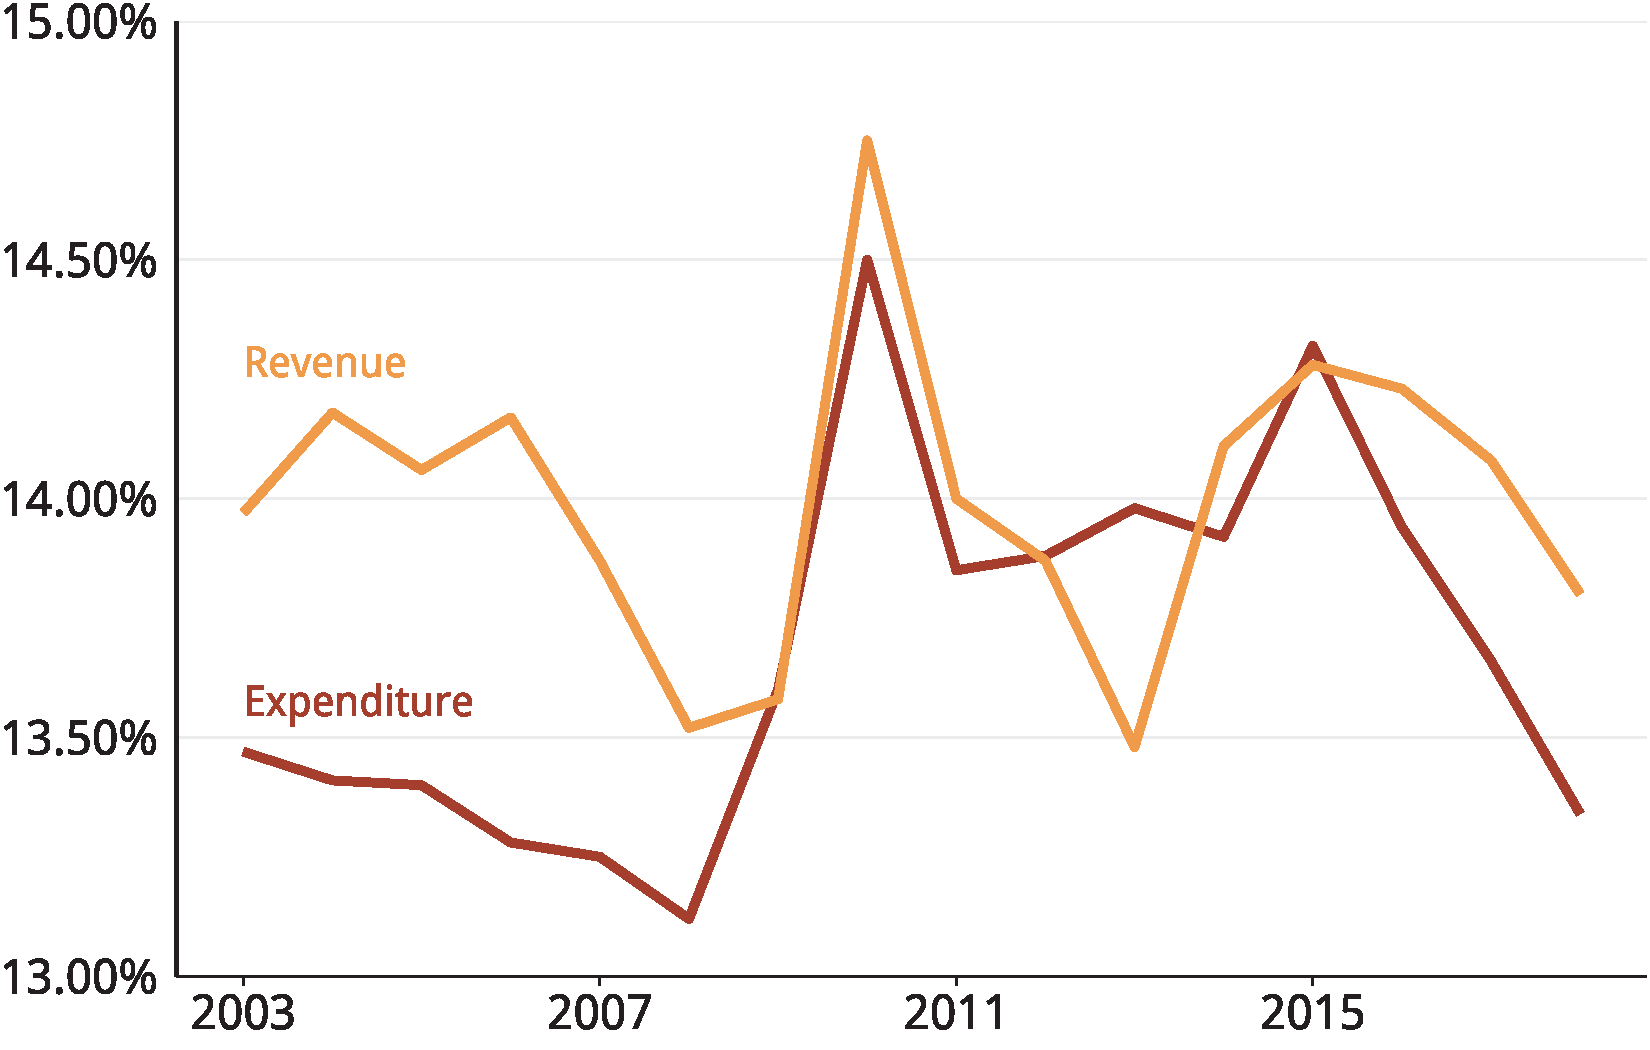
\includegraphics[width=11.000in,height=7.00in]{./b5-figure/FISCAL-Figure11-1} 

\end{knitrout}

\begin{knitrout}
\definecolor{shadecolor}{rgb}{0.969, 0.969, 0.969}\color{fgcolor}
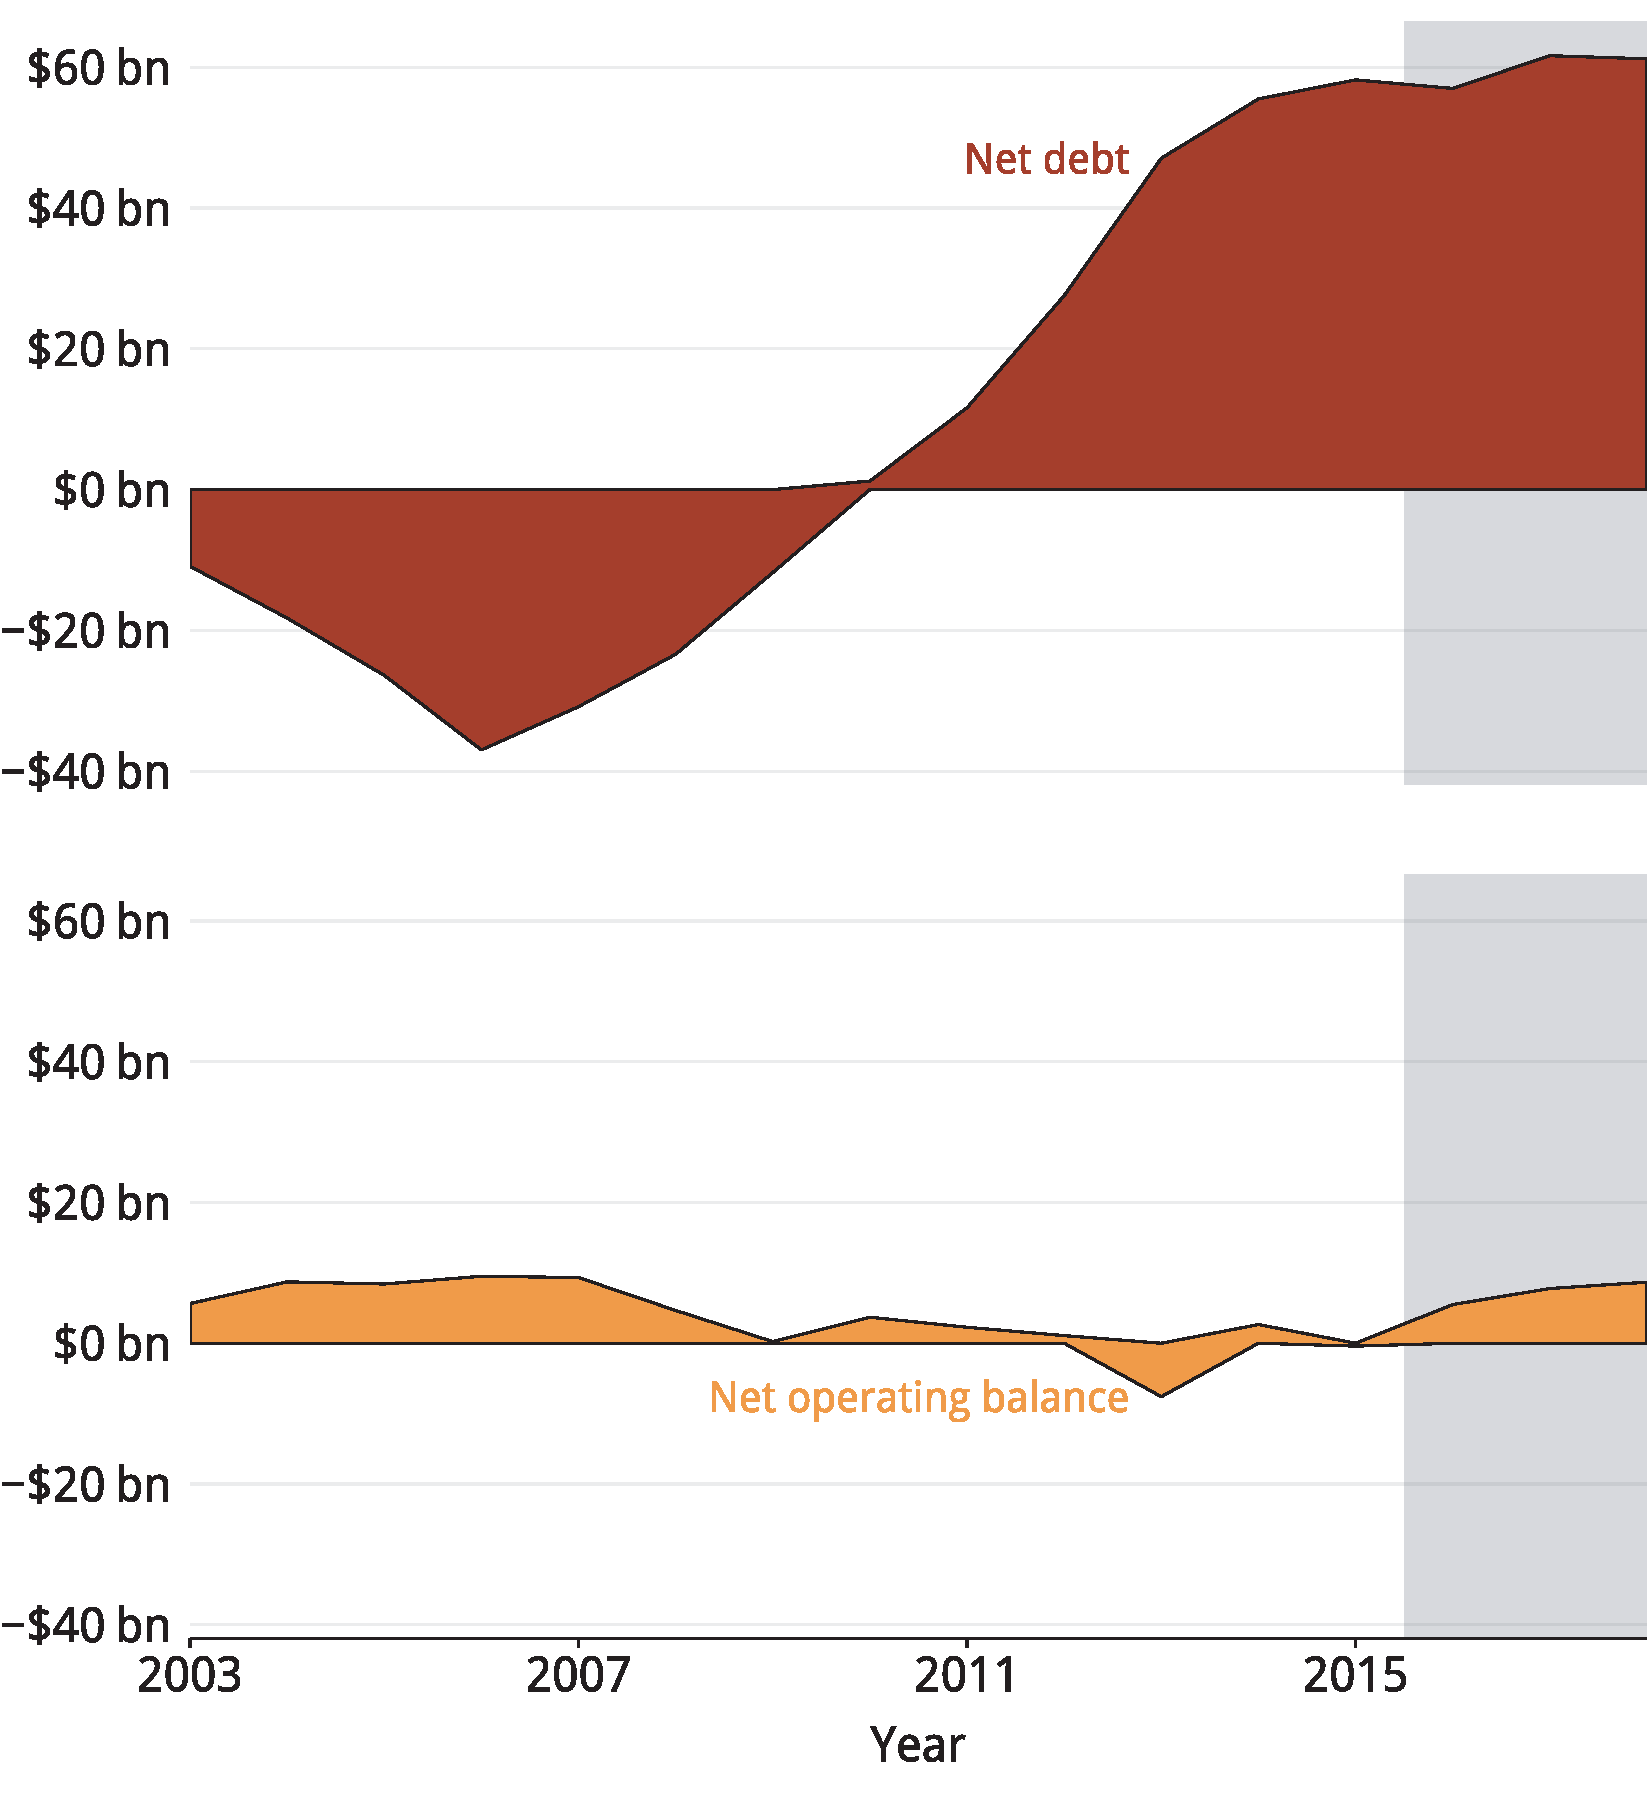
\includegraphics[width=11.000in,height=12in]{./b5-figure/FISCAL-Figure12-1} 

\end{knitrout}


\clearpage

\begin{knitrout}
\definecolor{shadecolor}{rgb}{0.969, 0.969, 0.969}\color{fgcolor}
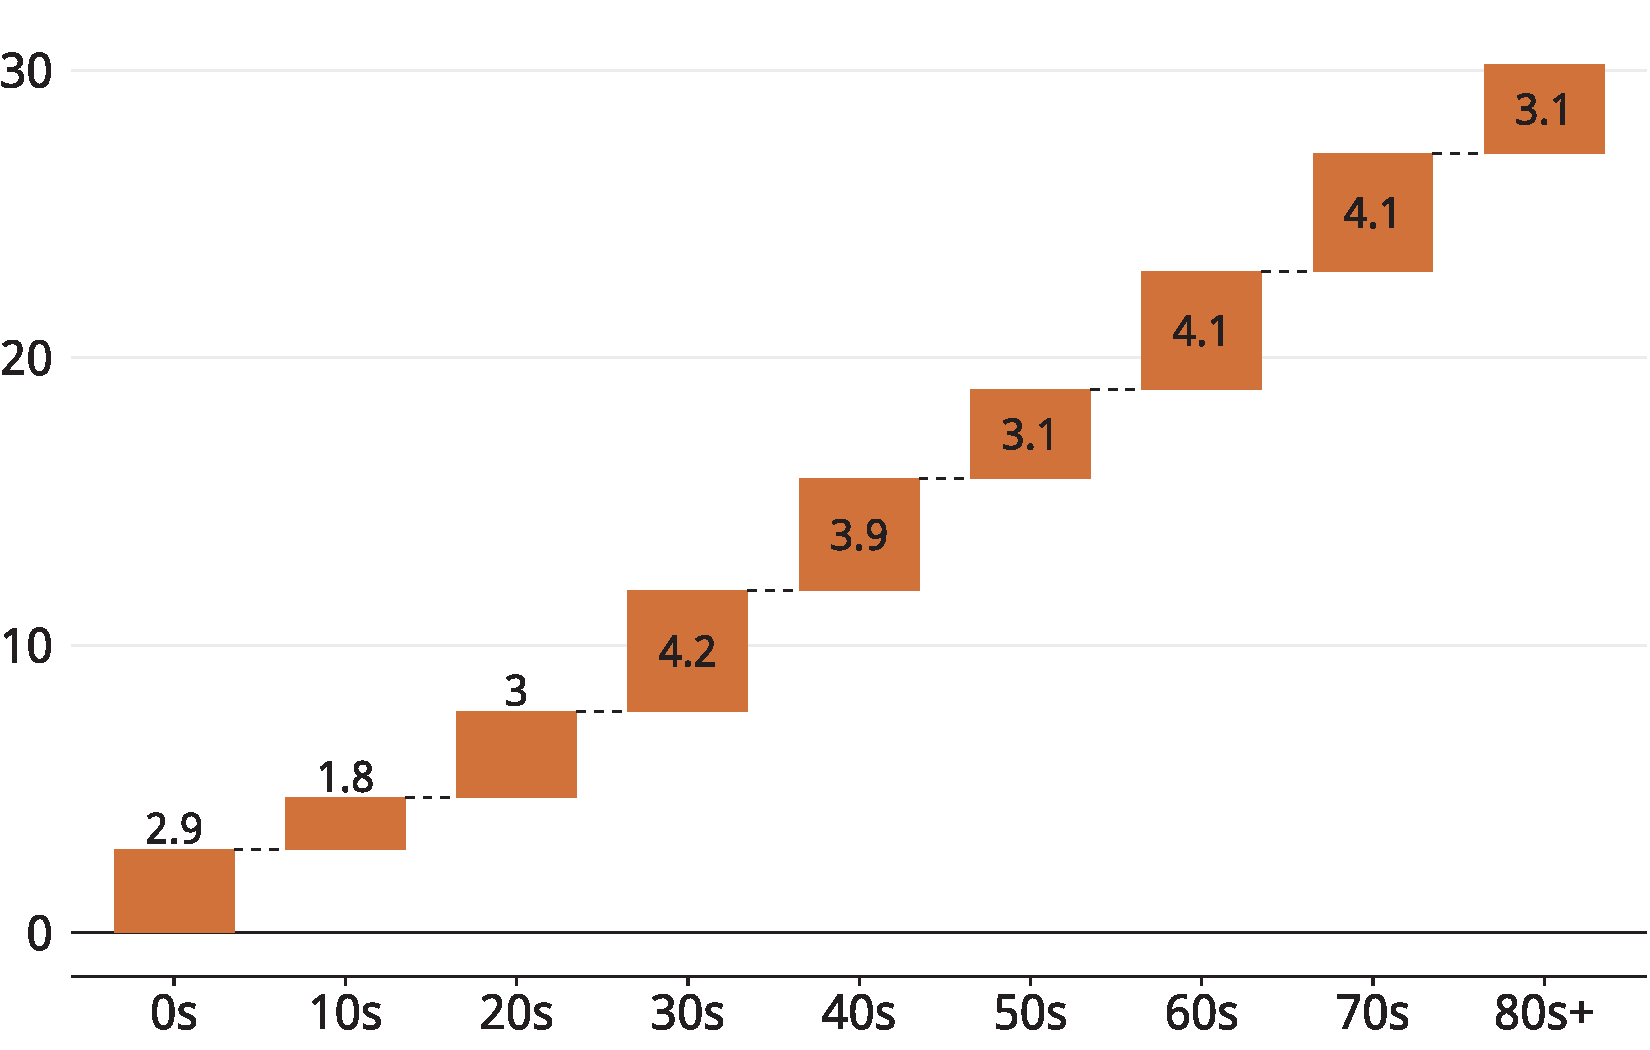
\includegraphics[width=11.000in,height=7.00in]{./b5-figure/FISCAL-Figure13-pre-1} 
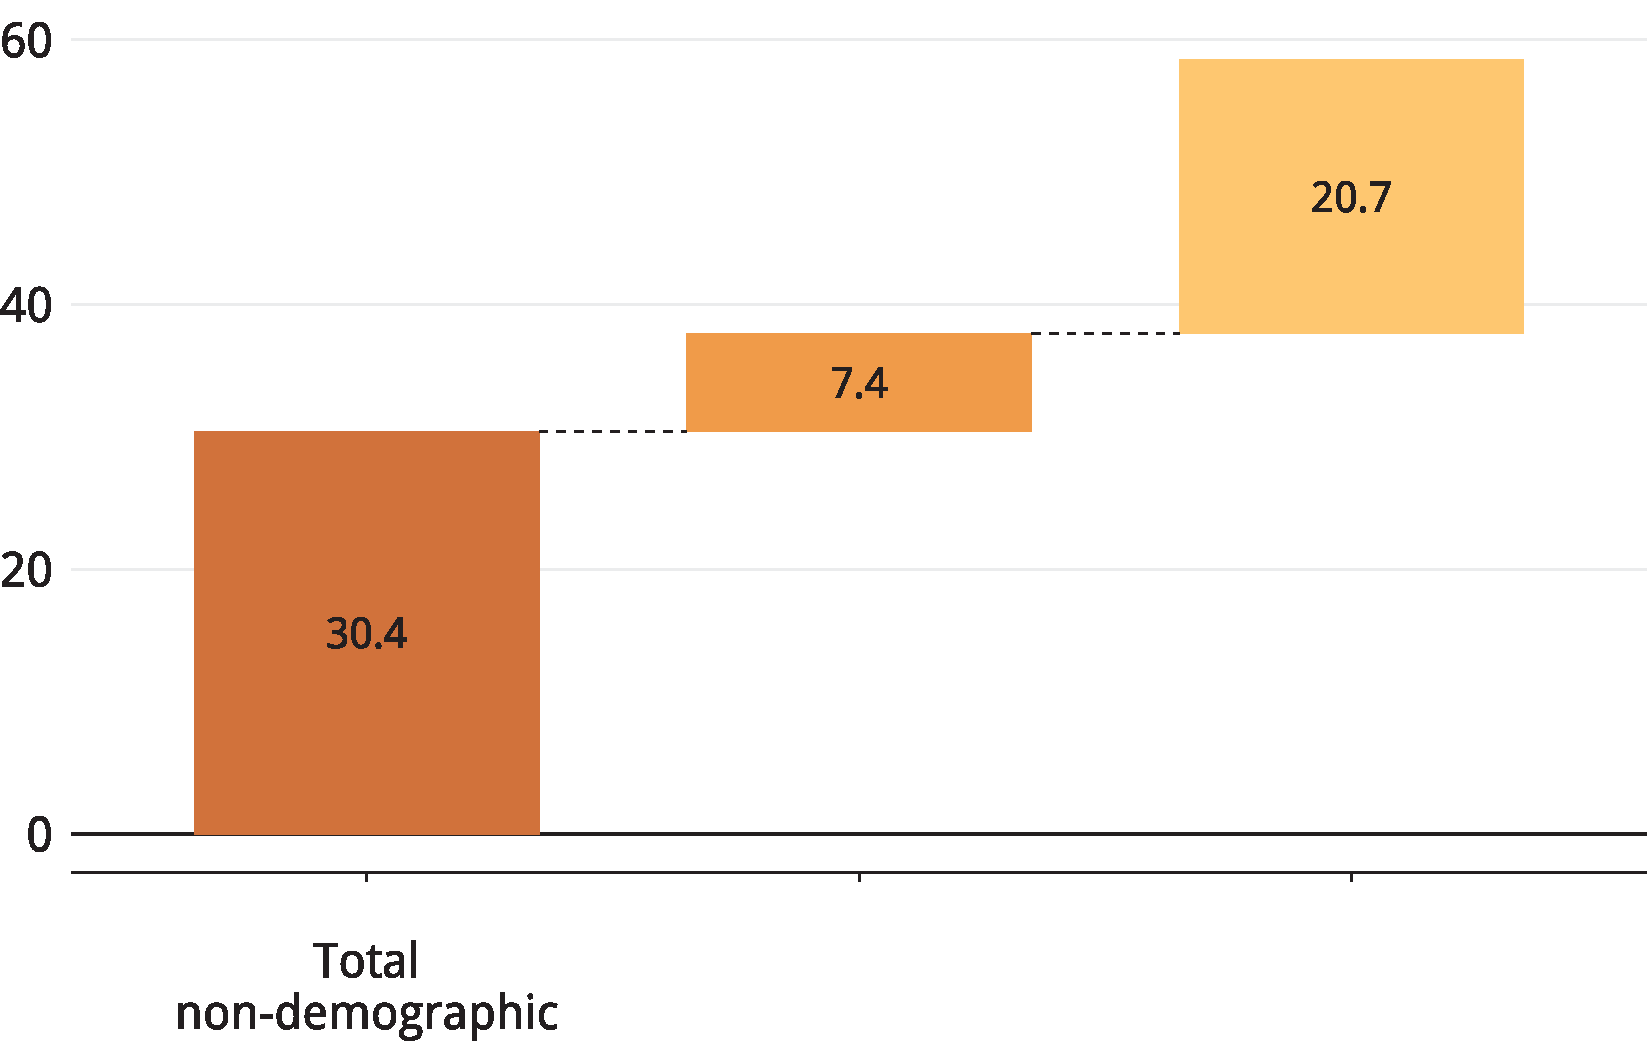
\includegraphics[width=11.000in,height=7.00in]{./b5-figure/FISCAL-Figure13-pre-2} 

\end{knitrout}
\begin{knitrout}
\definecolor{shadecolor}{rgb}{0.969, 0.969, 0.969}\color{fgcolor}
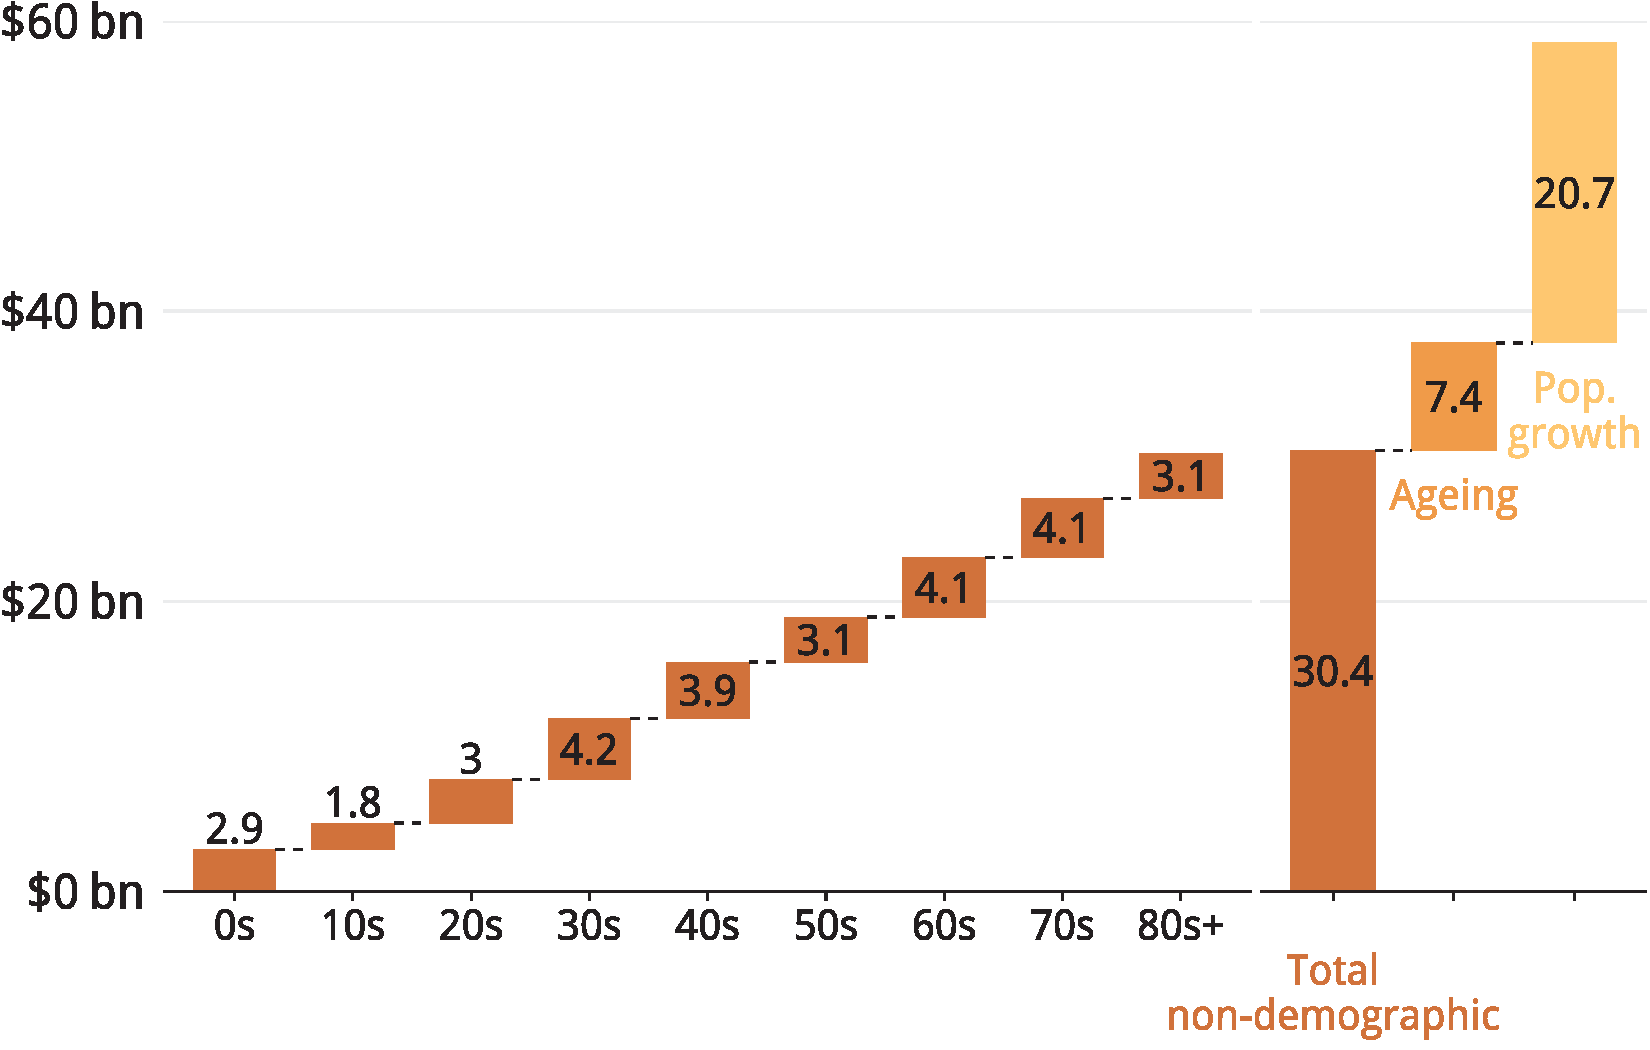
\includegraphics[width=11.000in,height=7.00in]{./b5-figure/FISCAL-Figure13-1} 

\end{knitrout}


\clearpage
\begin{knitrout}
\definecolor{shadecolor}{rgb}{0.969, 0.969, 0.969}\color{fgcolor}
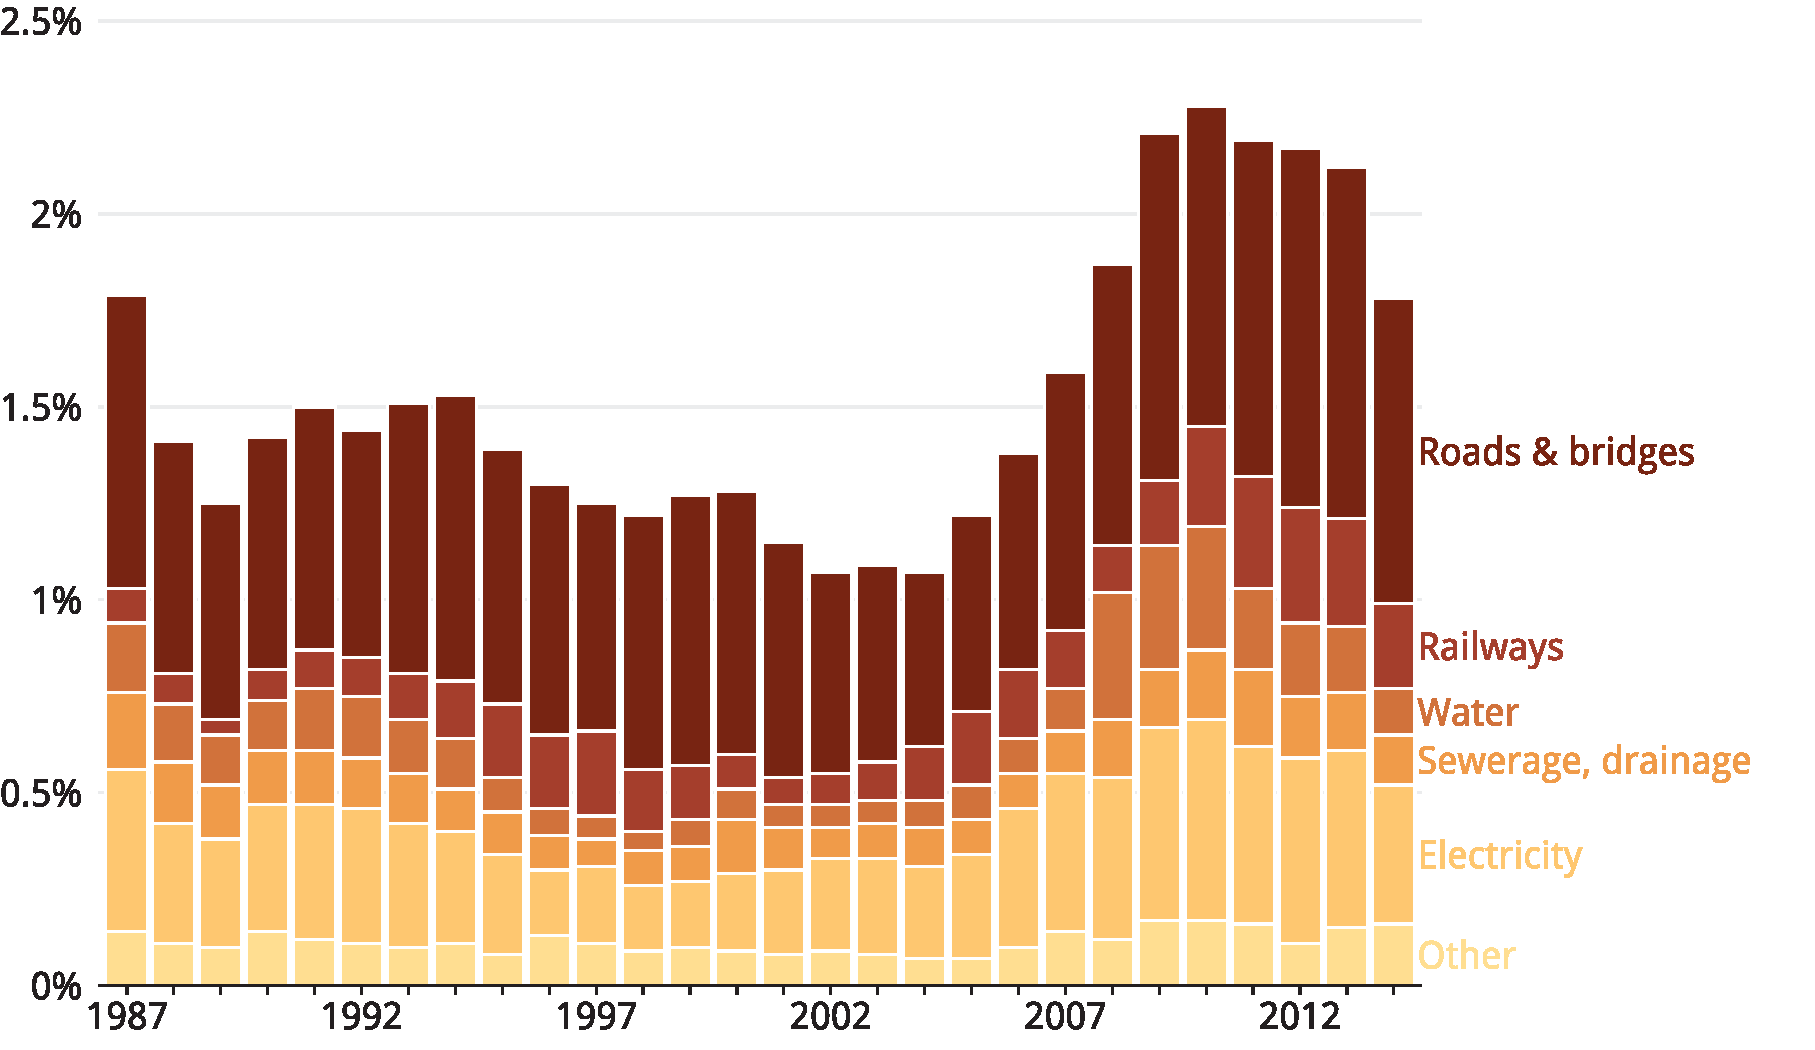
\includegraphics[width=12.1in,height=7in]{./b5-figure/FISCAL-Figure14-1} 

\end{knitrout}

\begin{knitrout}
\definecolor{shadecolor}{rgb}{0.969, 0.969, 0.969}\color{fgcolor}
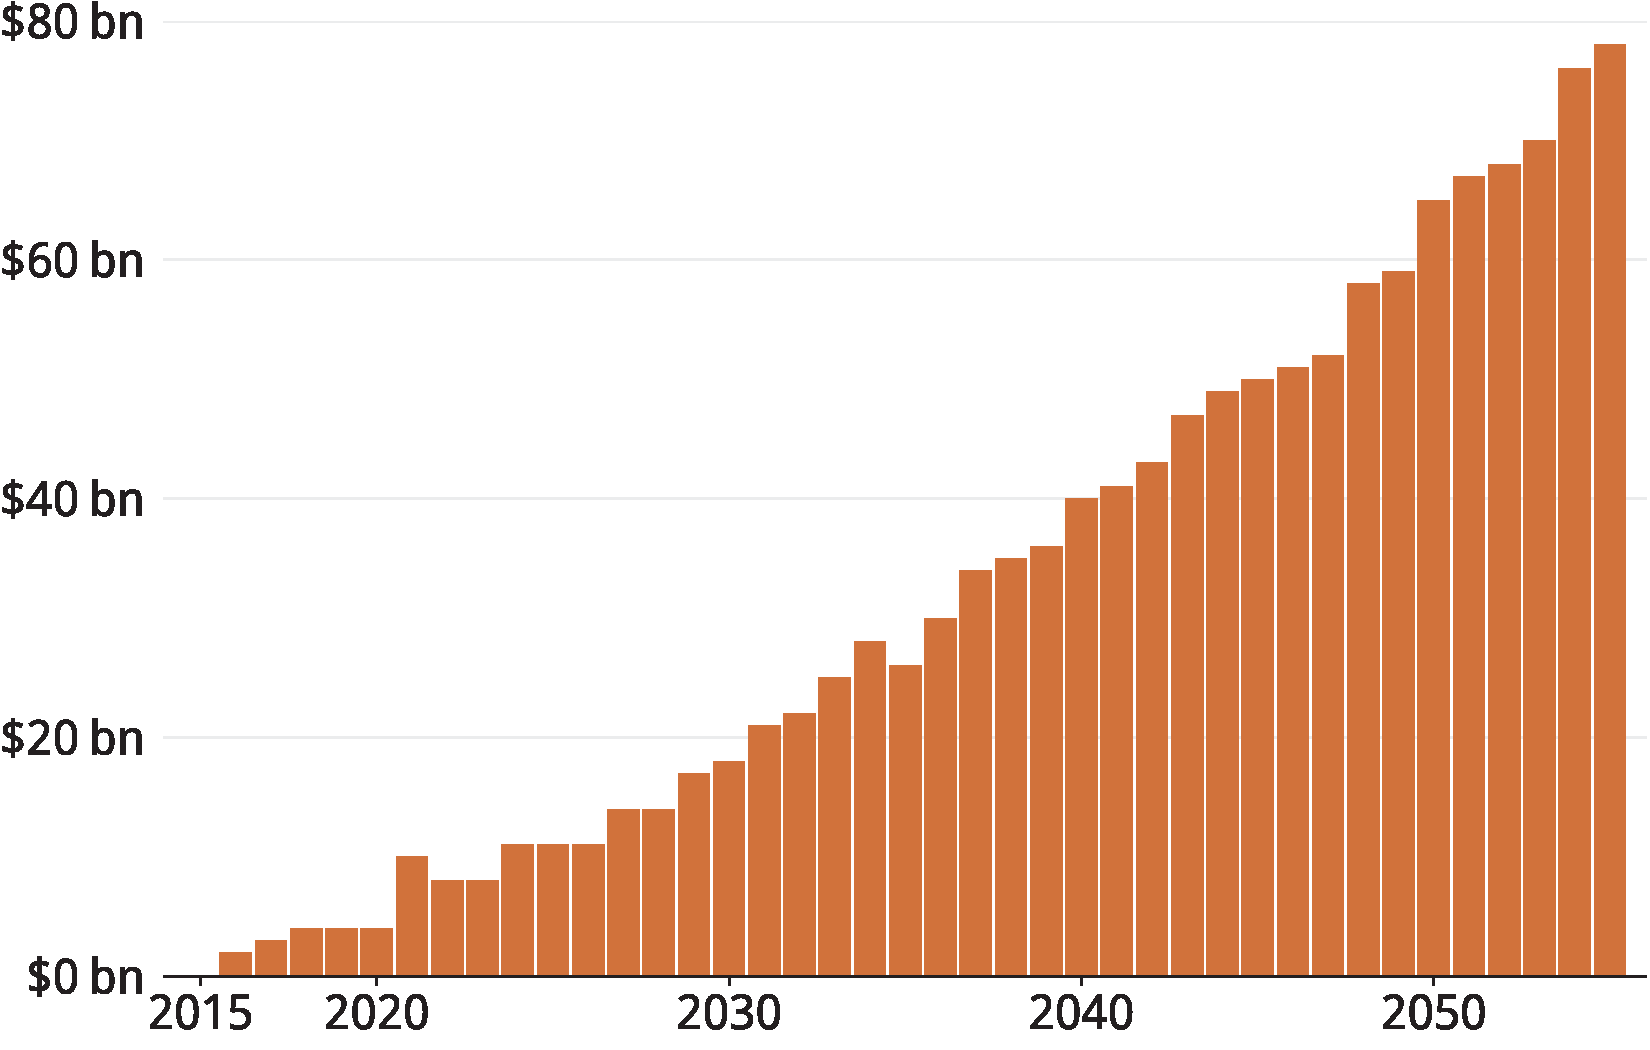
\includegraphics[width=11.000in,height=7.00in]{./b5-figure/FISCAL-Figure15-1} 

\end{knitrout}

\section{Property}



\begin{knitrout}
\definecolor{shadecolor}{rgb}{0.969, 0.969, 0.969}\color{fgcolor}
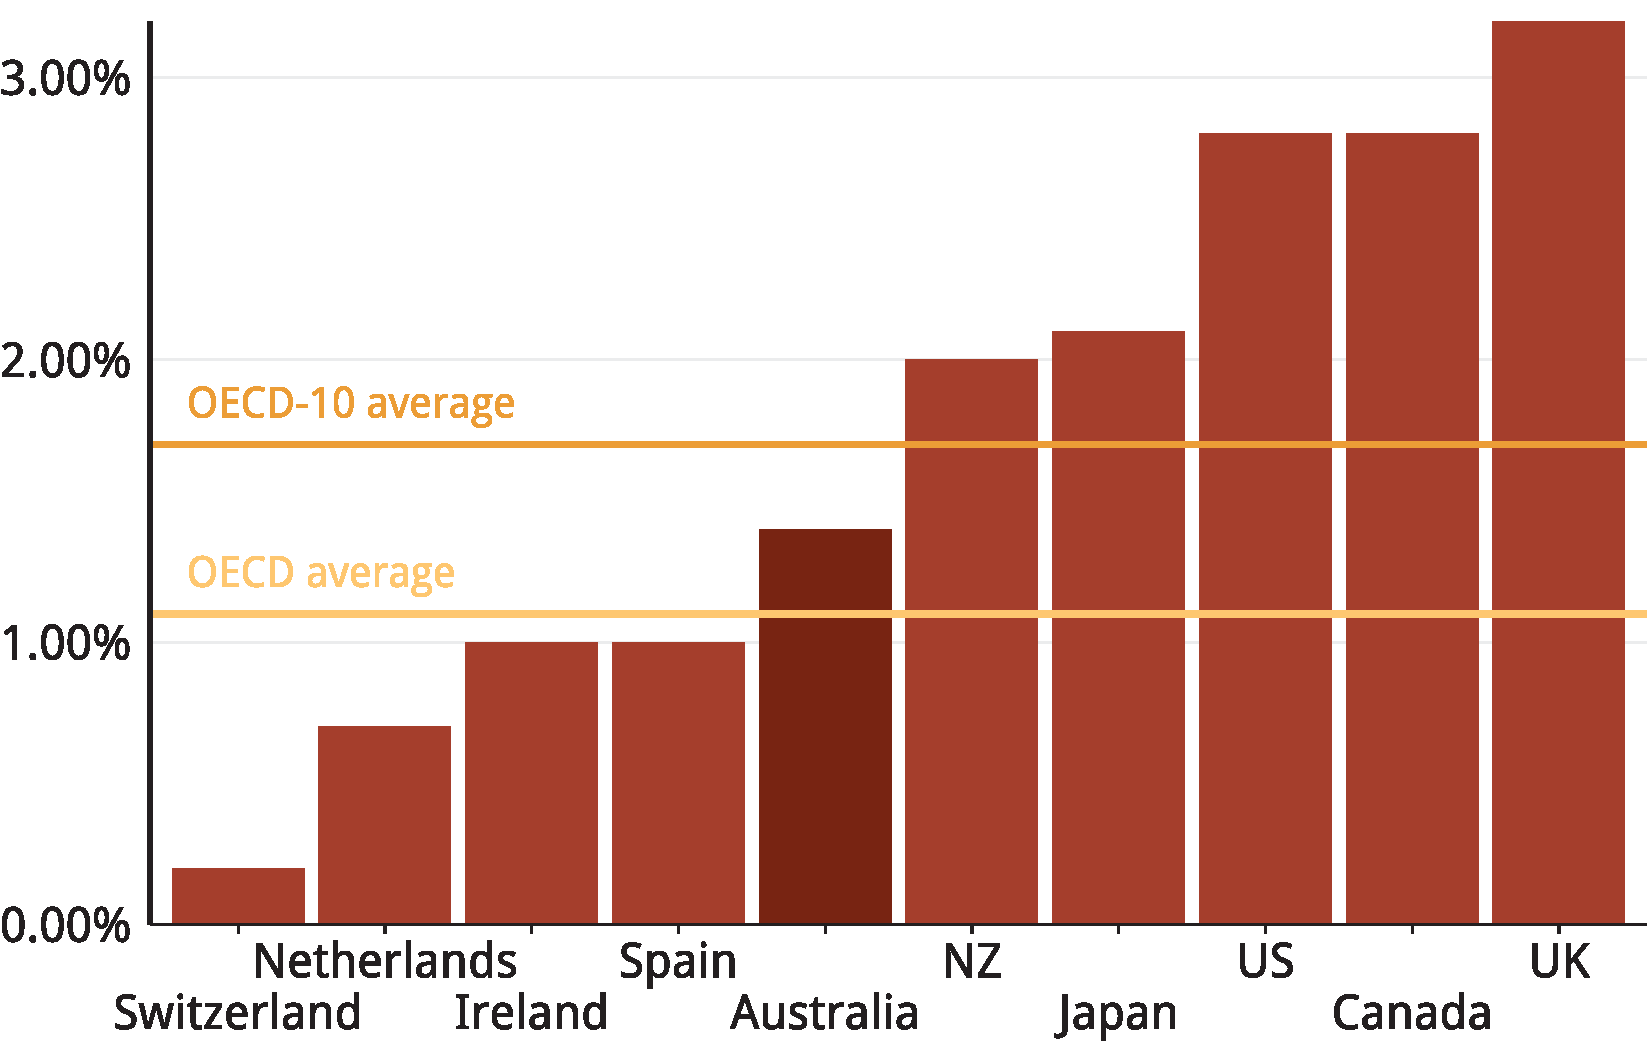
\includegraphics[width=11.000in,height=7.00in]{./Property-taxes/atlas/figure/PROP-Figure1-1} 

\end{knitrout}

\begin{knitrout}
\definecolor{shadecolor}{rgb}{0.969, 0.969, 0.969}\color{fgcolor}
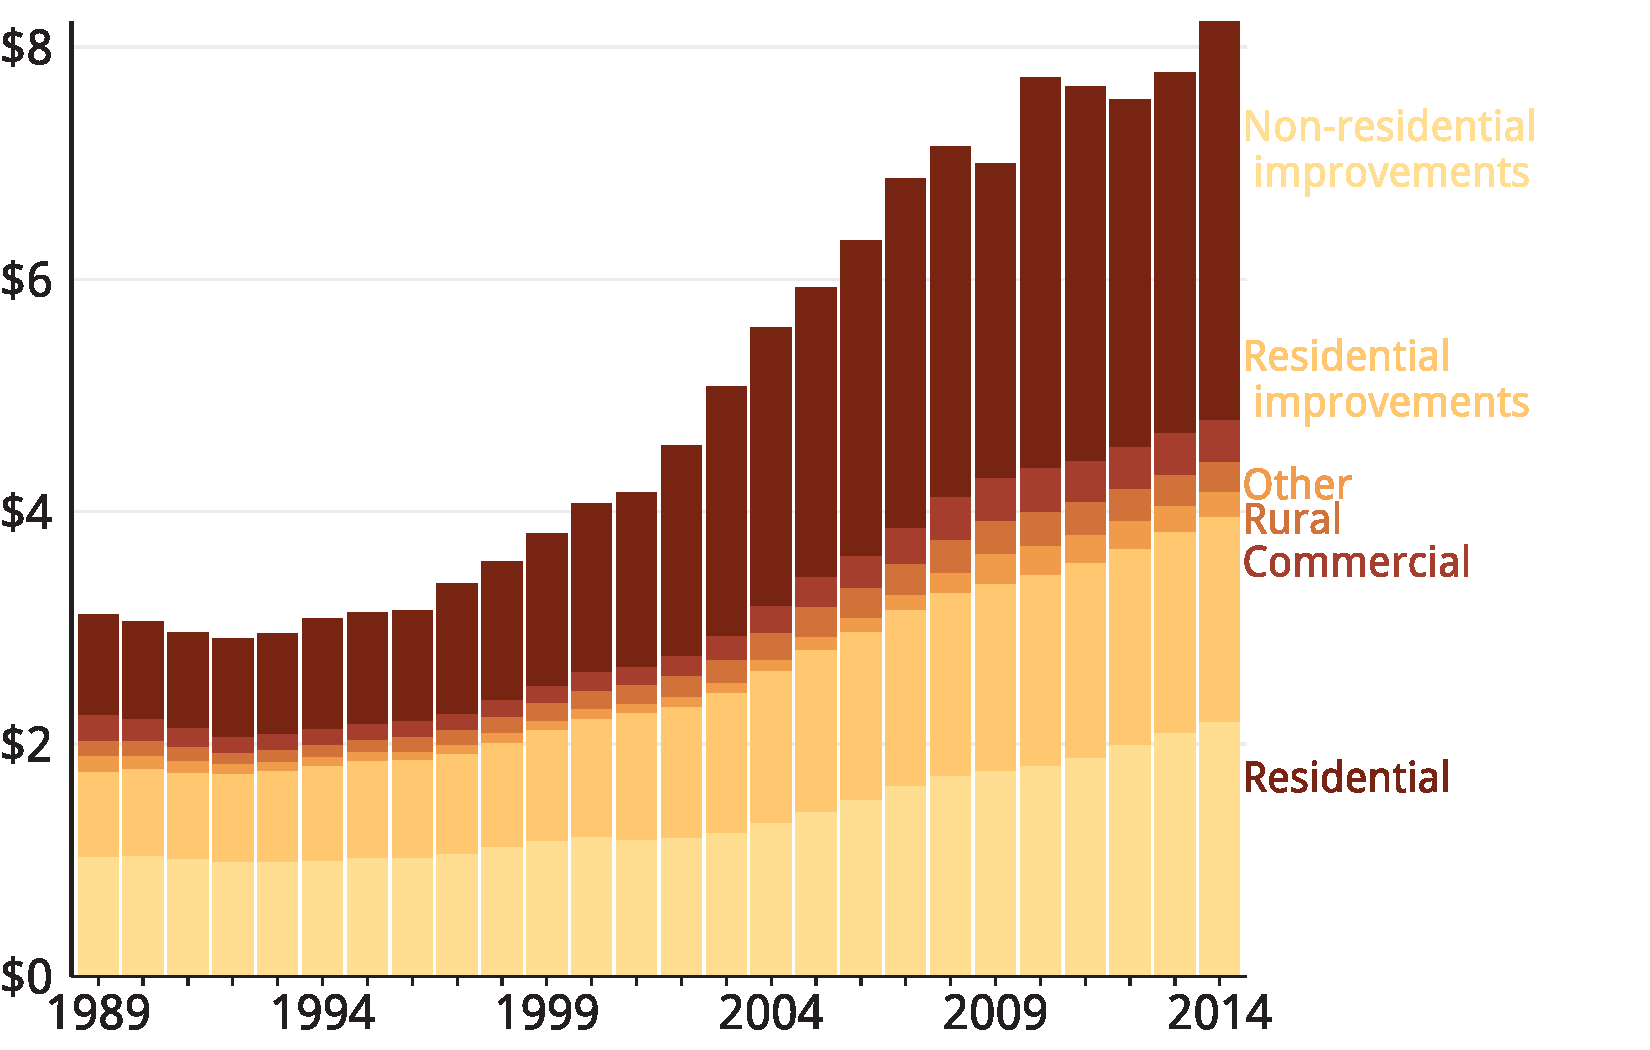
\includegraphics[width=11.000in,height=7.00in]{./Property-taxes/atlas/figure/PROP-Figure2-1} 

\end{knitrout}

\clearpage
\begin{knitrout}
\definecolor{shadecolor}{rgb}{0.969, 0.969, 0.969}\color{fgcolor}
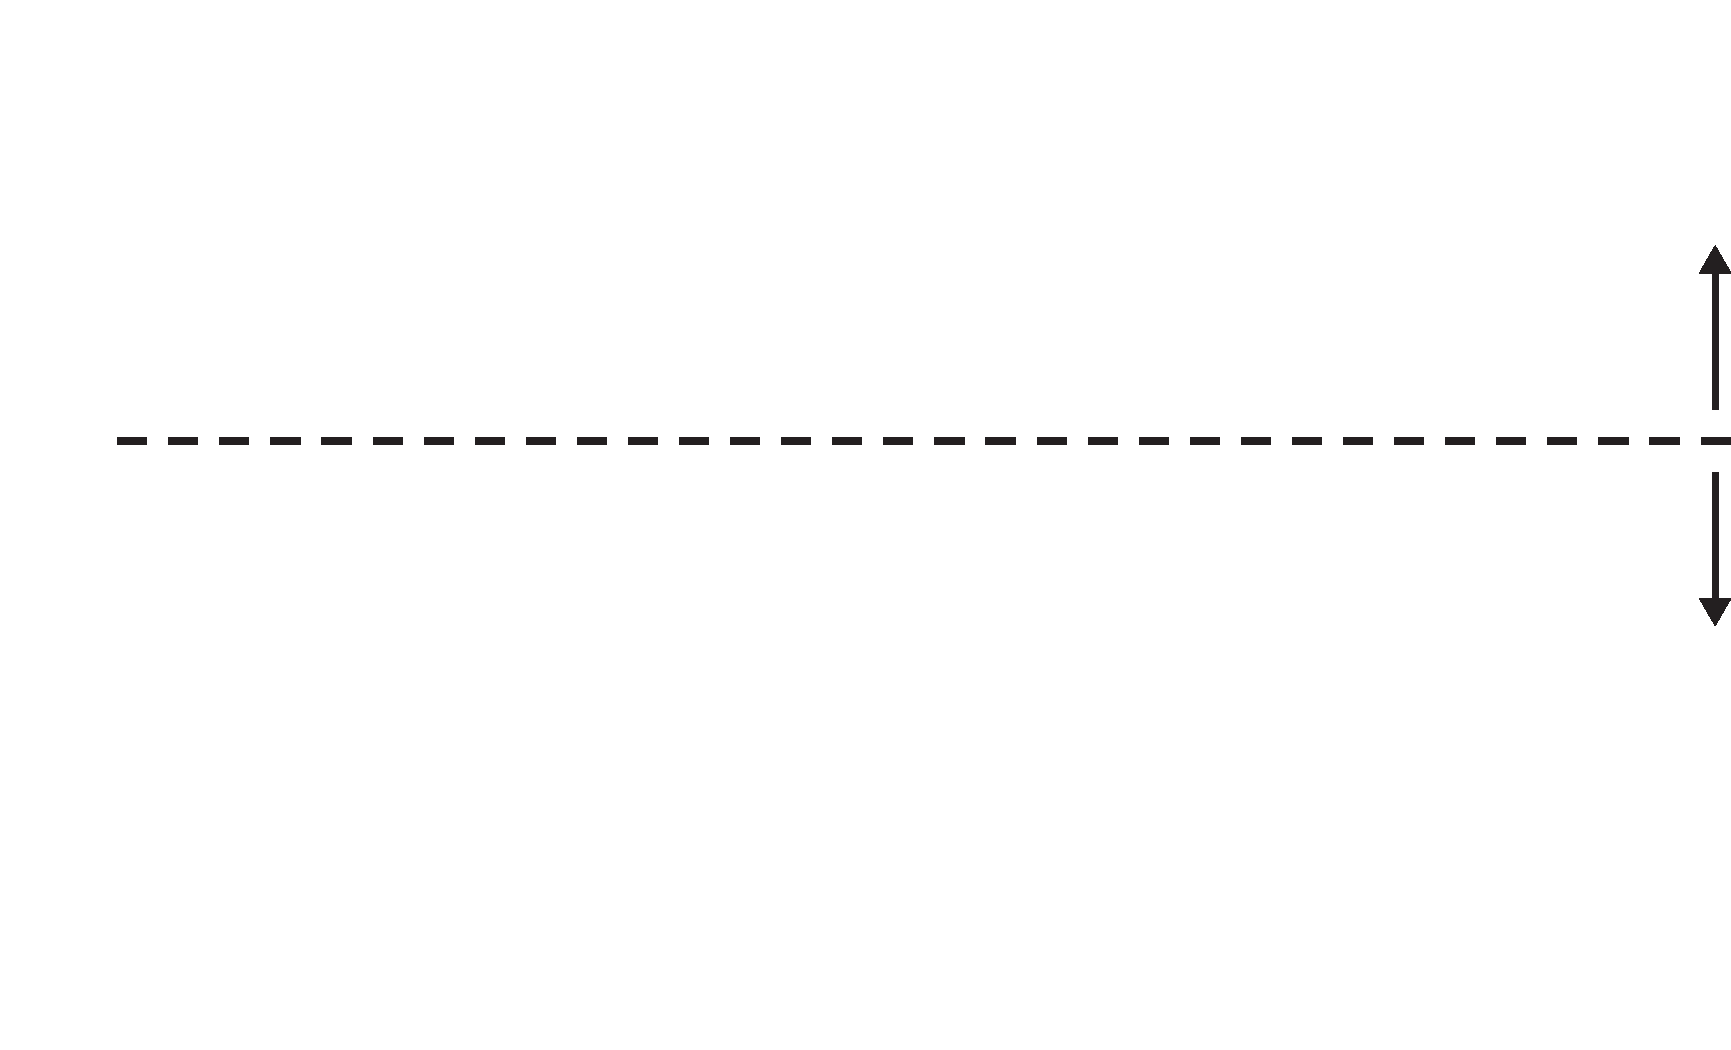
\includegraphics[width=11.55in,height=7.00in]{./Property-taxes/atlas/figure/PROP-Figure3-textwidth-1} 

\end{knitrout}
\clearpage
\begin{knitrout}
\definecolor{shadecolor}{rgb}{0.969, 0.969, 0.969}\color{fgcolor}
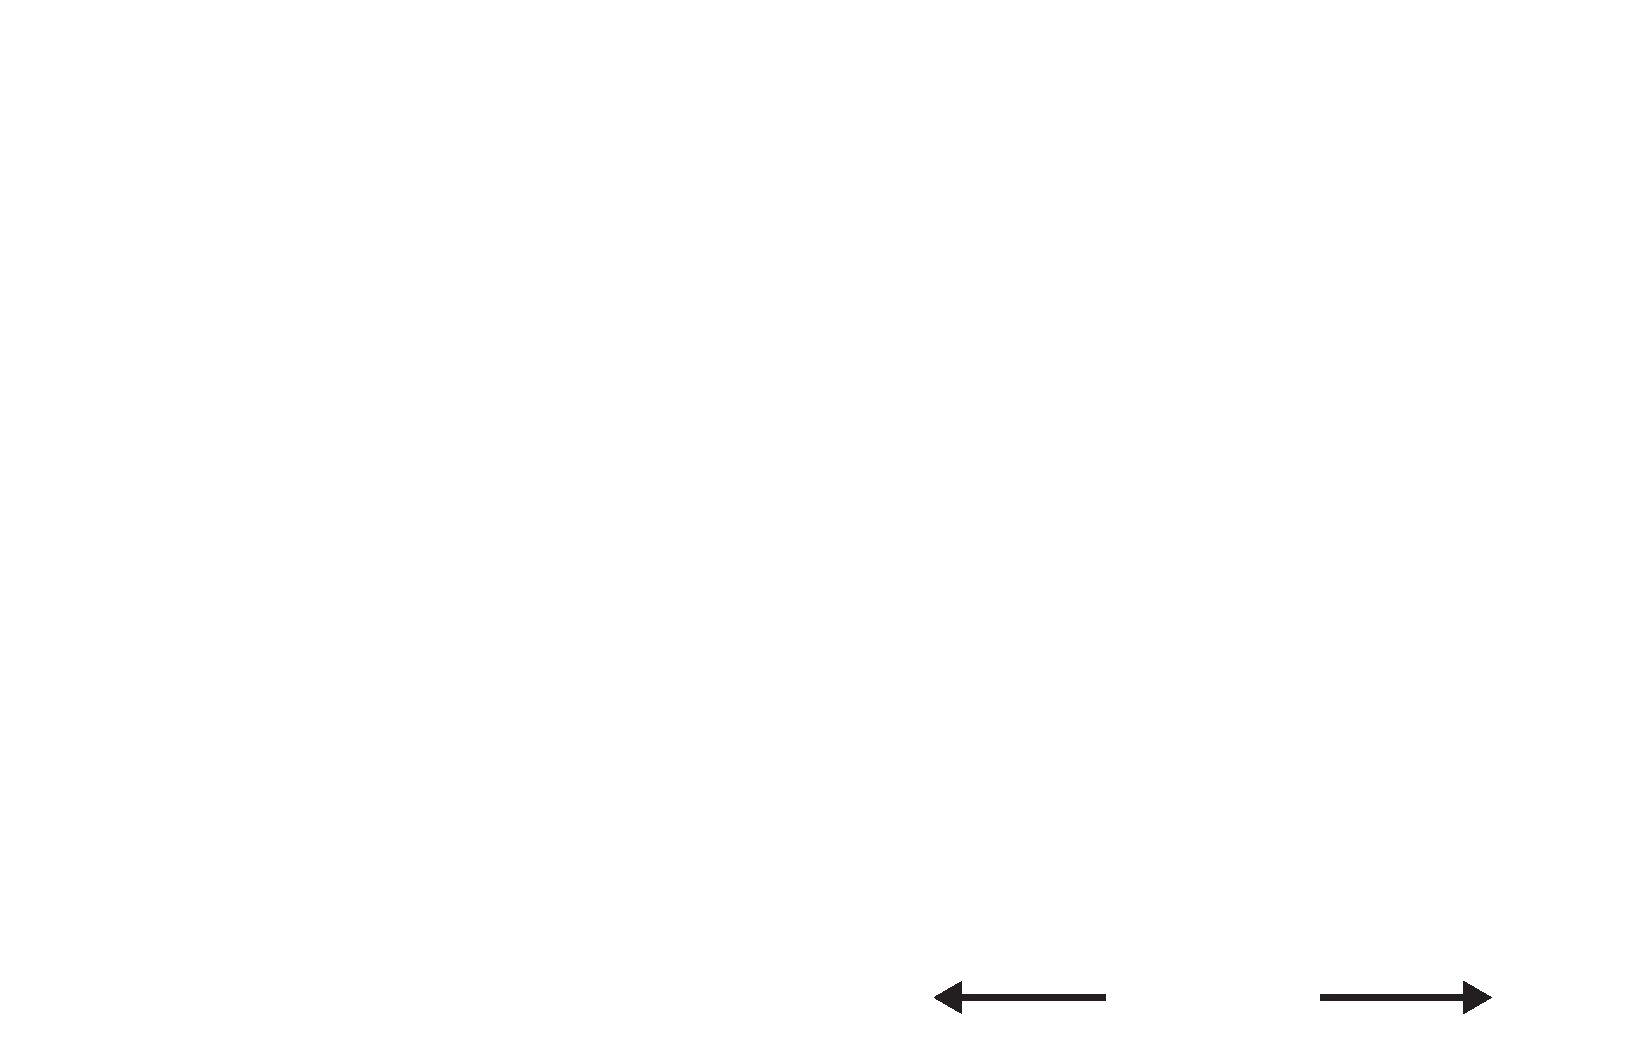
\includegraphics[width=11.000in,height=7.00in]{./Property-taxes/atlas/figure/PROP-Figure3-flipped-1} 

\end{knitrout}

\clearpage
\begin{knitrout}
\definecolor{shadecolor}{rgb}{0.969, 0.969, 0.969}\color{fgcolor}
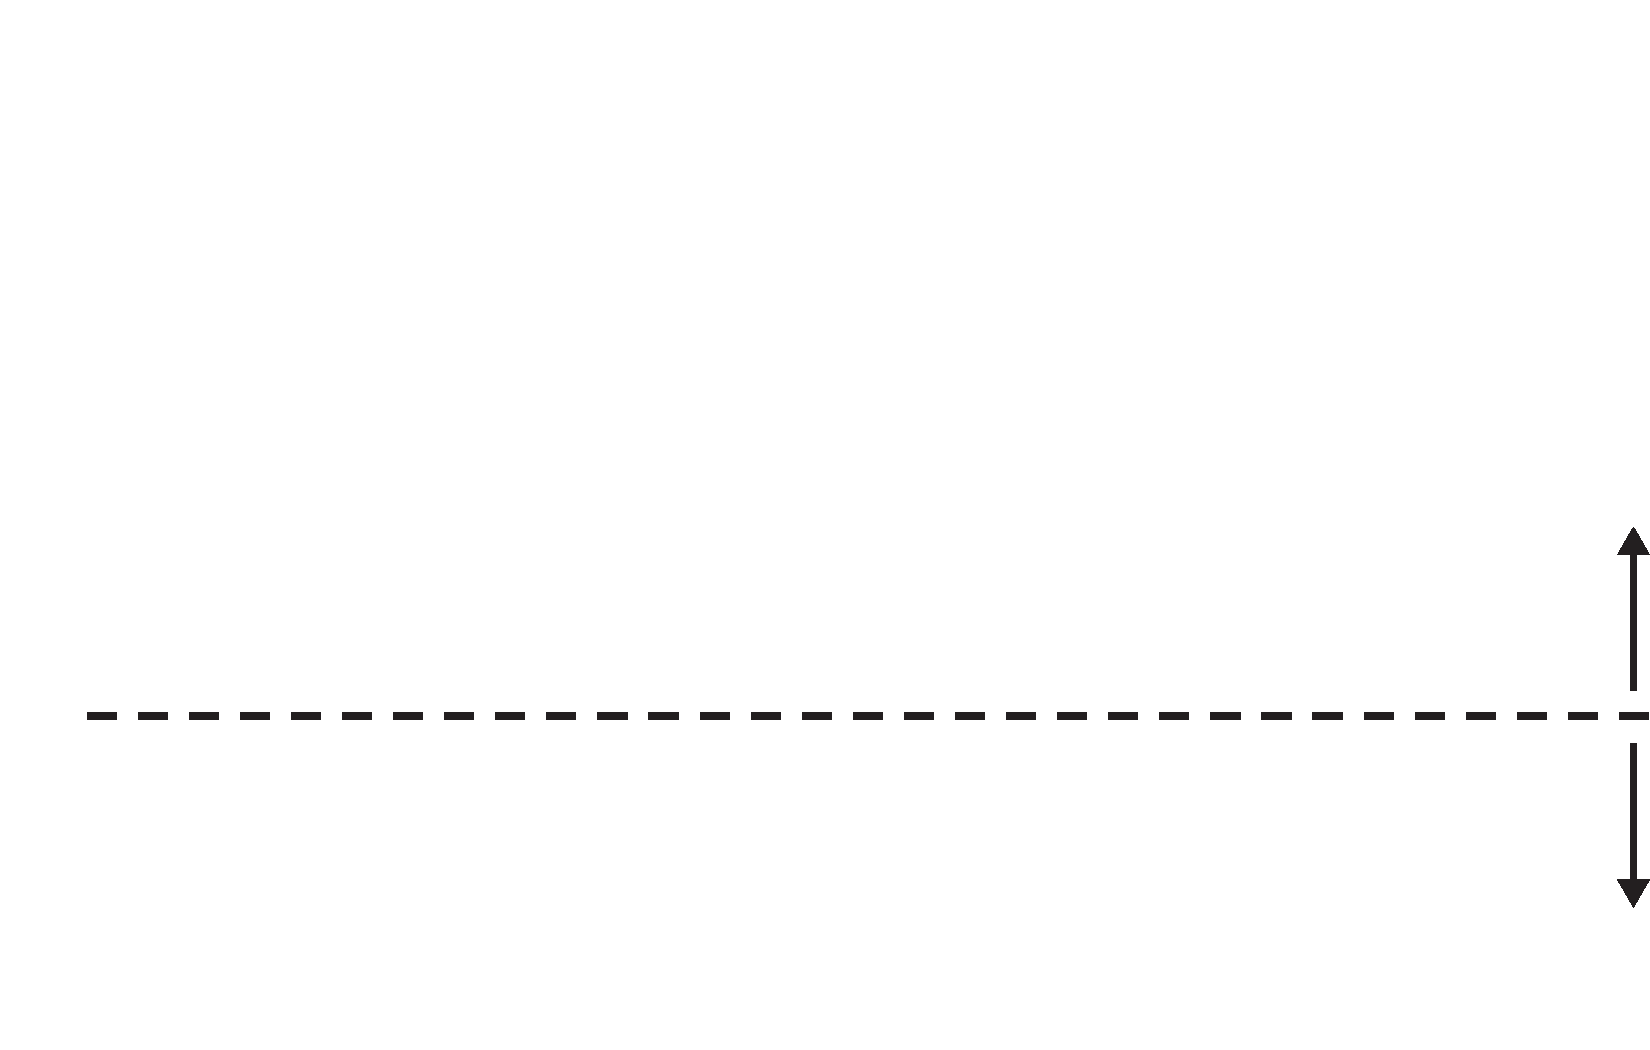
\includegraphics[width=11.000in,height=7.00in]{./Property-taxes/atlas/figure/PROP-Figure4-1} 

\end{knitrout}
\clearpage

\begin{knitrout}
\definecolor{shadecolor}{rgb}{0.969, 0.969, 0.969}\color{fgcolor}
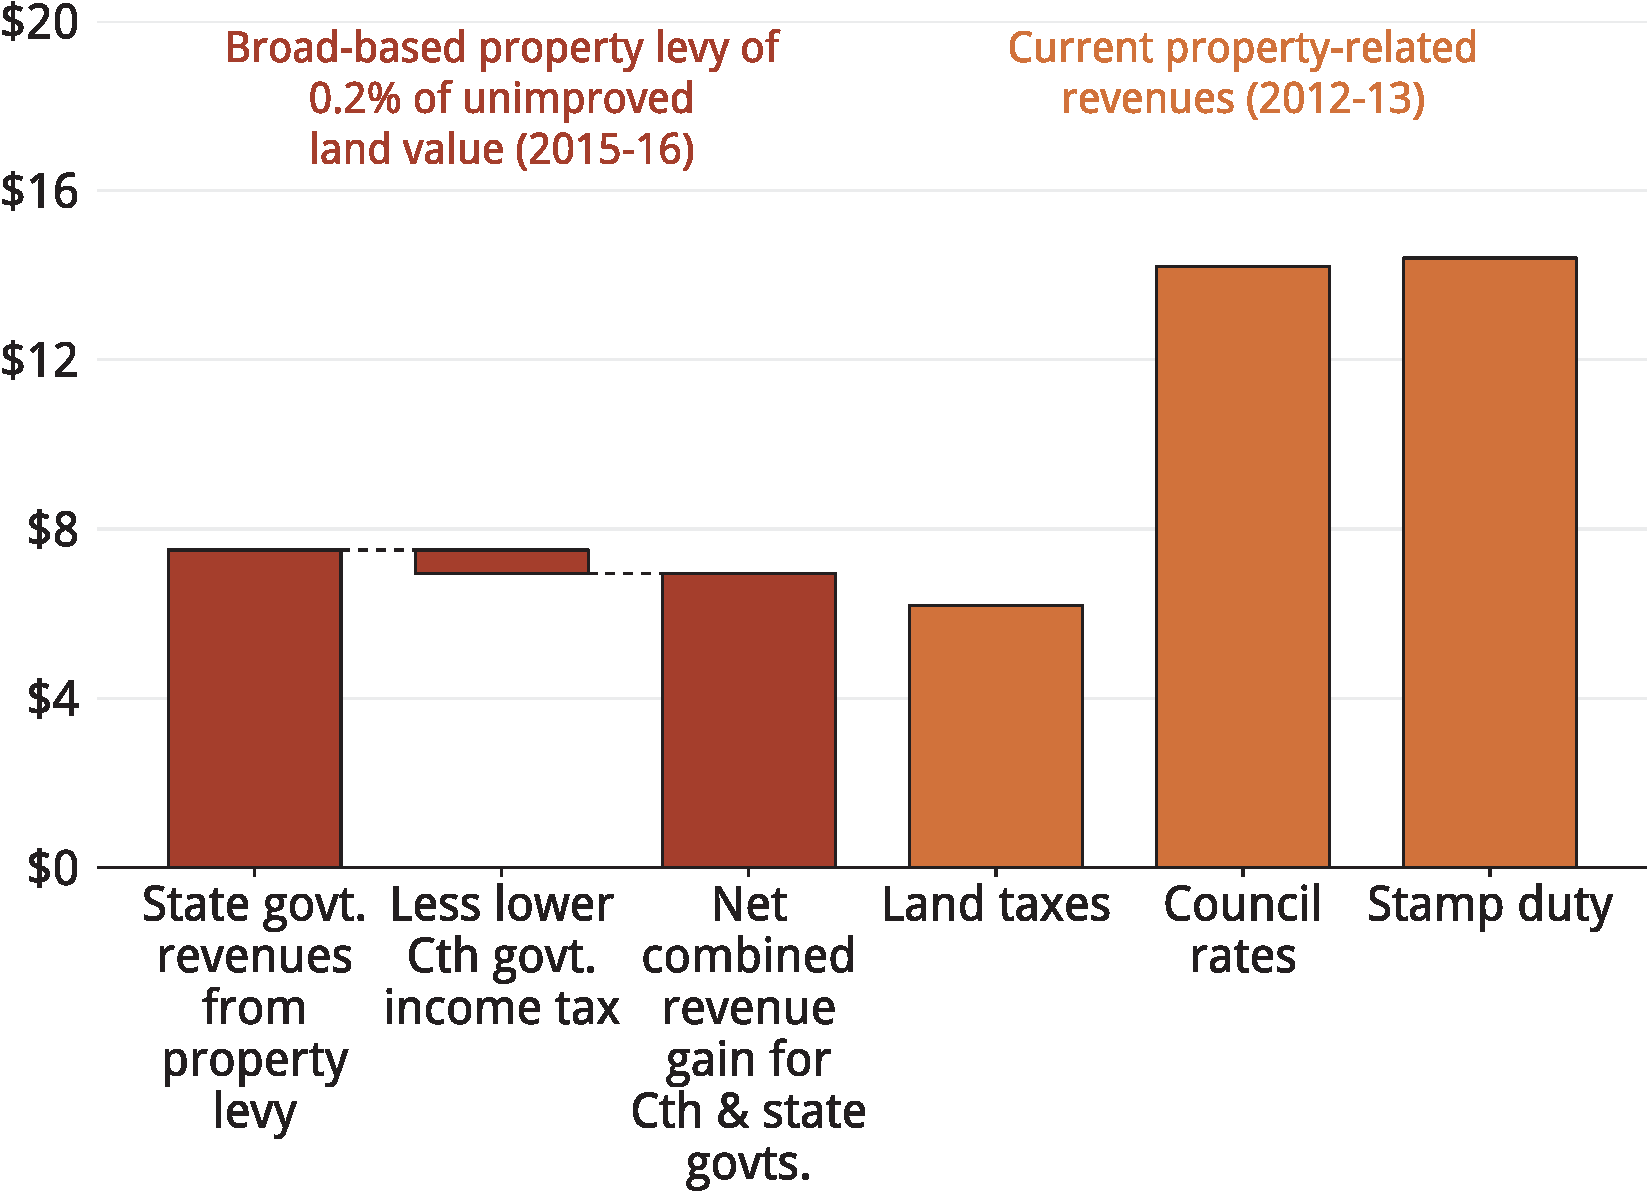
\includegraphics[width=11.000in,height=8in]{./Property-taxes/atlas/figure/PROP-Figure5-1} 

\end{knitrout}

\begin{knitrout}
\definecolor{shadecolor}{rgb}{0.969, 0.969, 0.969}\color{fgcolor}\begin{kframe}
\begin{verbatim}
##  [1] 0.7lines                   0cm                       
##  [3] 0cm                        0cm                       
##  [5] 0cm                        0cm                       
##  [7] 1null                      sum(0.3lines, 1grobheight)
##  [9] 0cm                        0cm                       
## [11] 0pt                        0.5lines
\end{verbatim}
\end{kframe}
\end{knitrout}
\clearpage
\begin{knitrout}
\definecolor{shadecolor}{rgb}{0.969, 0.969, 0.969}\color{fgcolor}\begin{kframe}


{\ttfamily\noindent\bfseries\color{errorcolor}{\#\# Error in theme(axis.title.x = element\_blank(), legend.position = c(0, : formal argument "{}legend.justification"{} matched by multiple actual arguments}}\end{kframe}
\end{knitrout}

\clearpage
\begin{knitrout}
\definecolor{shadecolor}{rgb}{0.969, 0.969, 0.969}\color{fgcolor}
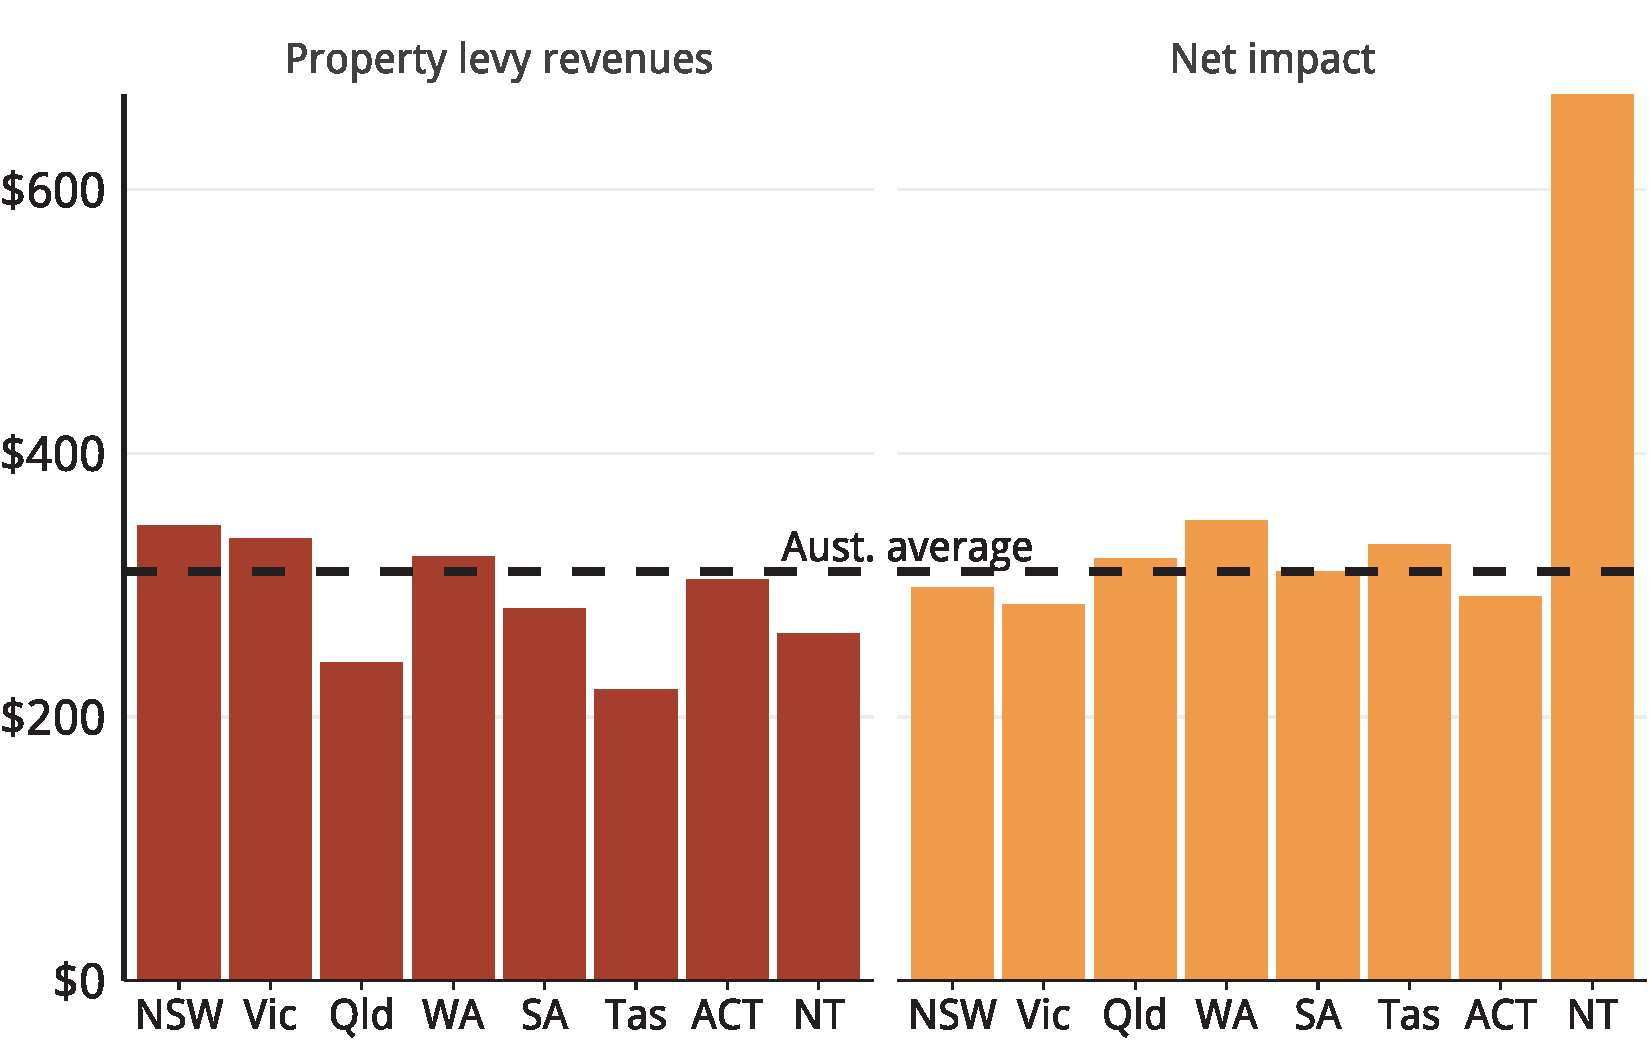
\includegraphics[width=11.000in,height=7.00in]{./Property-taxes/atlas/figure/PROP-Figure7-1} 

\end{knitrout}

\clearpage
\begin{knitrout}
\definecolor{shadecolor}{rgb}{0.969, 0.969, 0.969}\color{fgcolor}
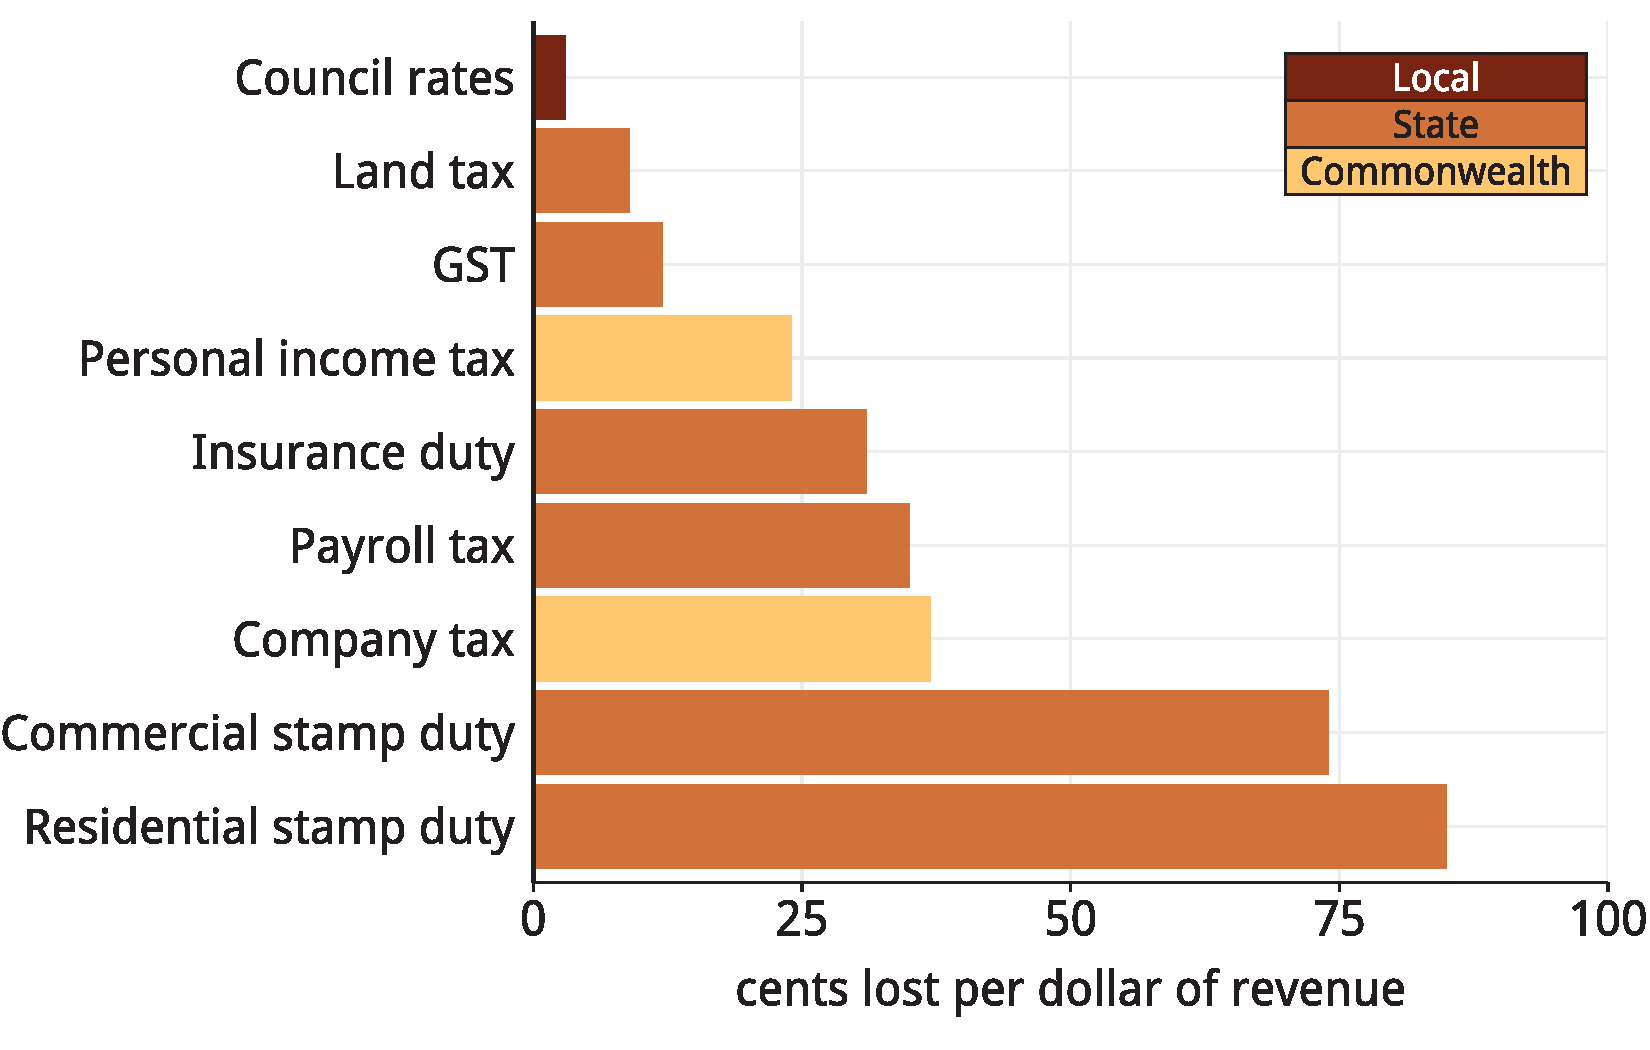
\includegraphics[width=11.000in,height=7.00in]{./Property-taxes/atlas/figure/PROP-Figure8-1} 

\end{knitrout}

\begin{knitrout}
\definecolor{shadecolor}{rgb}{0.969, 0.969, 0.969}\color{fgcolor}
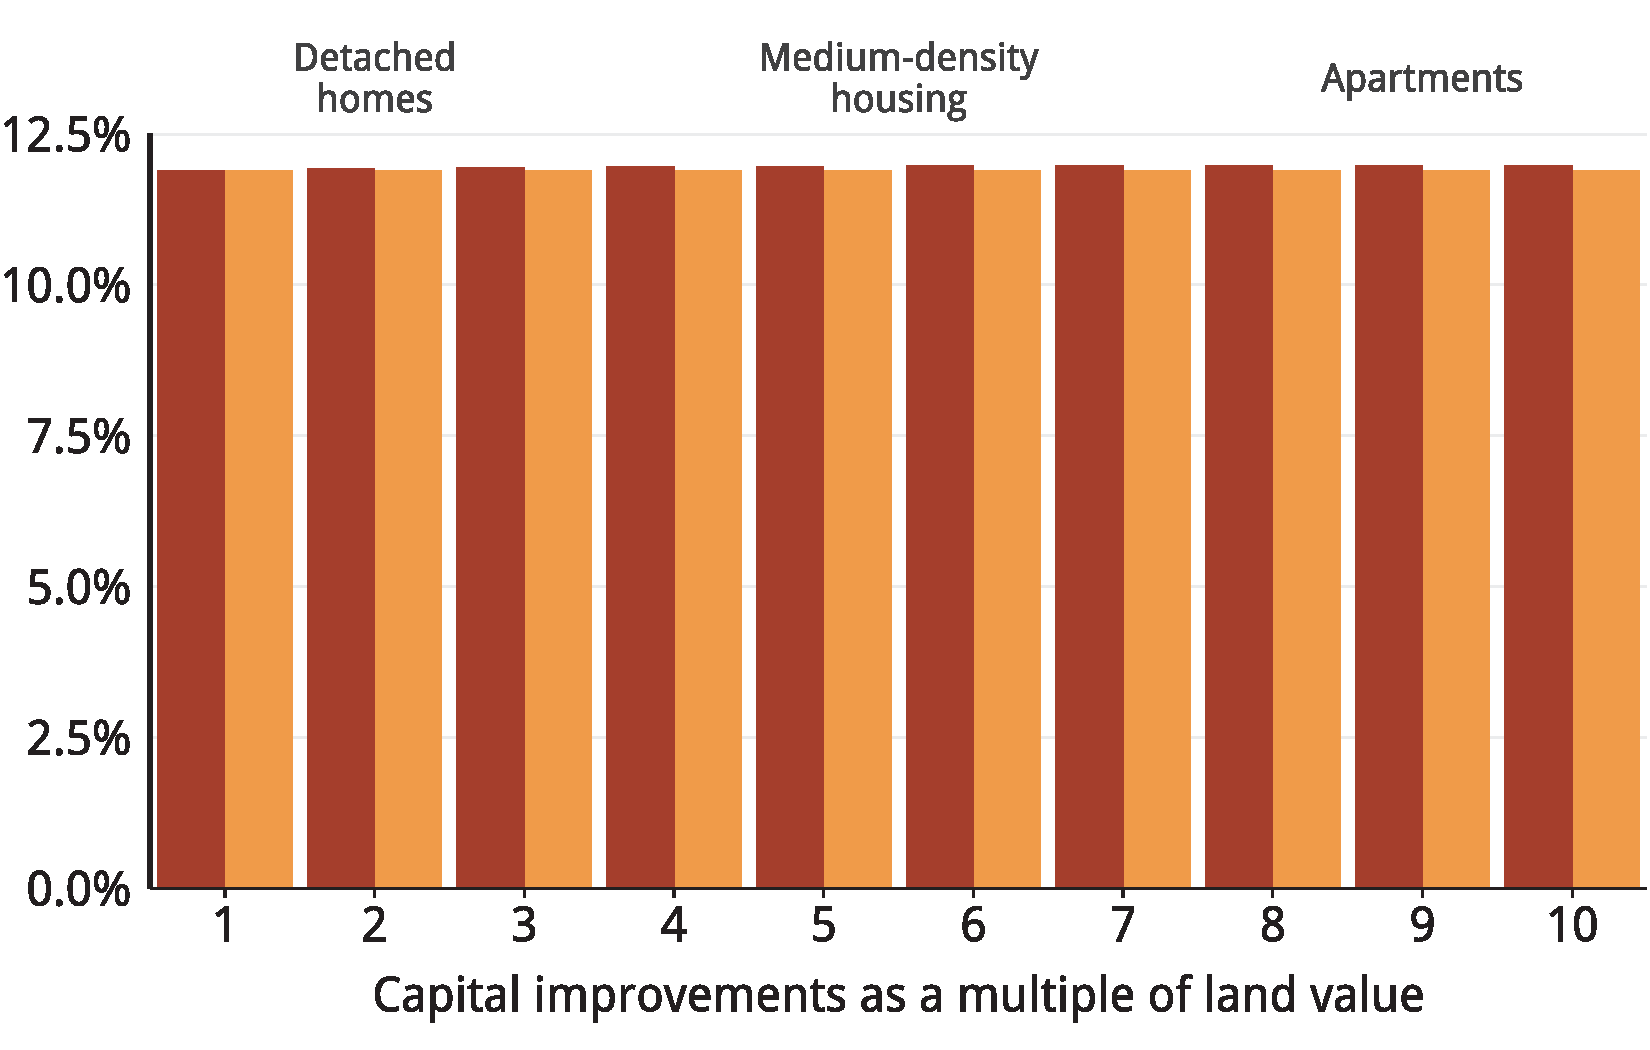
\includegraphics[width=11.000in,height=7.00in]{./Property-taxes/atlas/figure/PROP-Figure9-1} 

\end{knitrout}

\begin{knitrout}
\definecolor{shadecolor}{rgb}{0.969, 0.969, 0.969}\color{fgcolor}
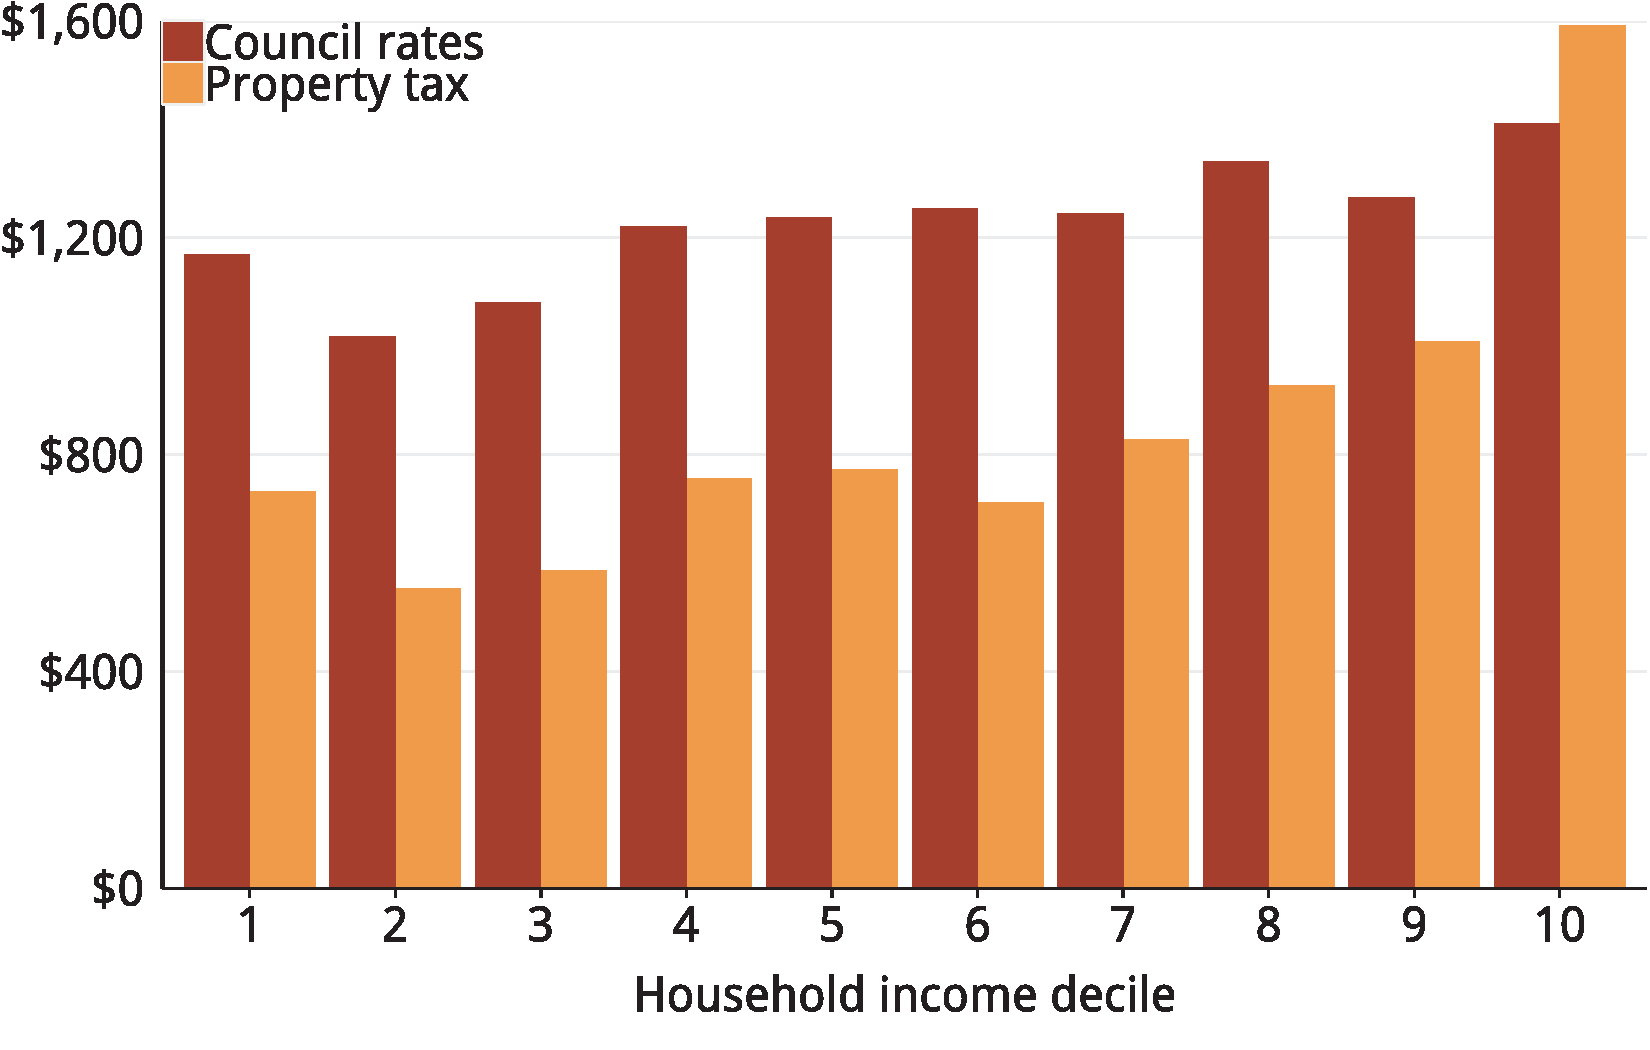
\includegraphics[width=11.000in,height=7.00in]{./Property-taxes/atlas/figure/PROP-Figure10-1} 

\end{knitrout}

\begin{knitrout}
\definecolor{shadecolor}{rgb}{0.969, 0.969, 0.969}\color{fgcolor}
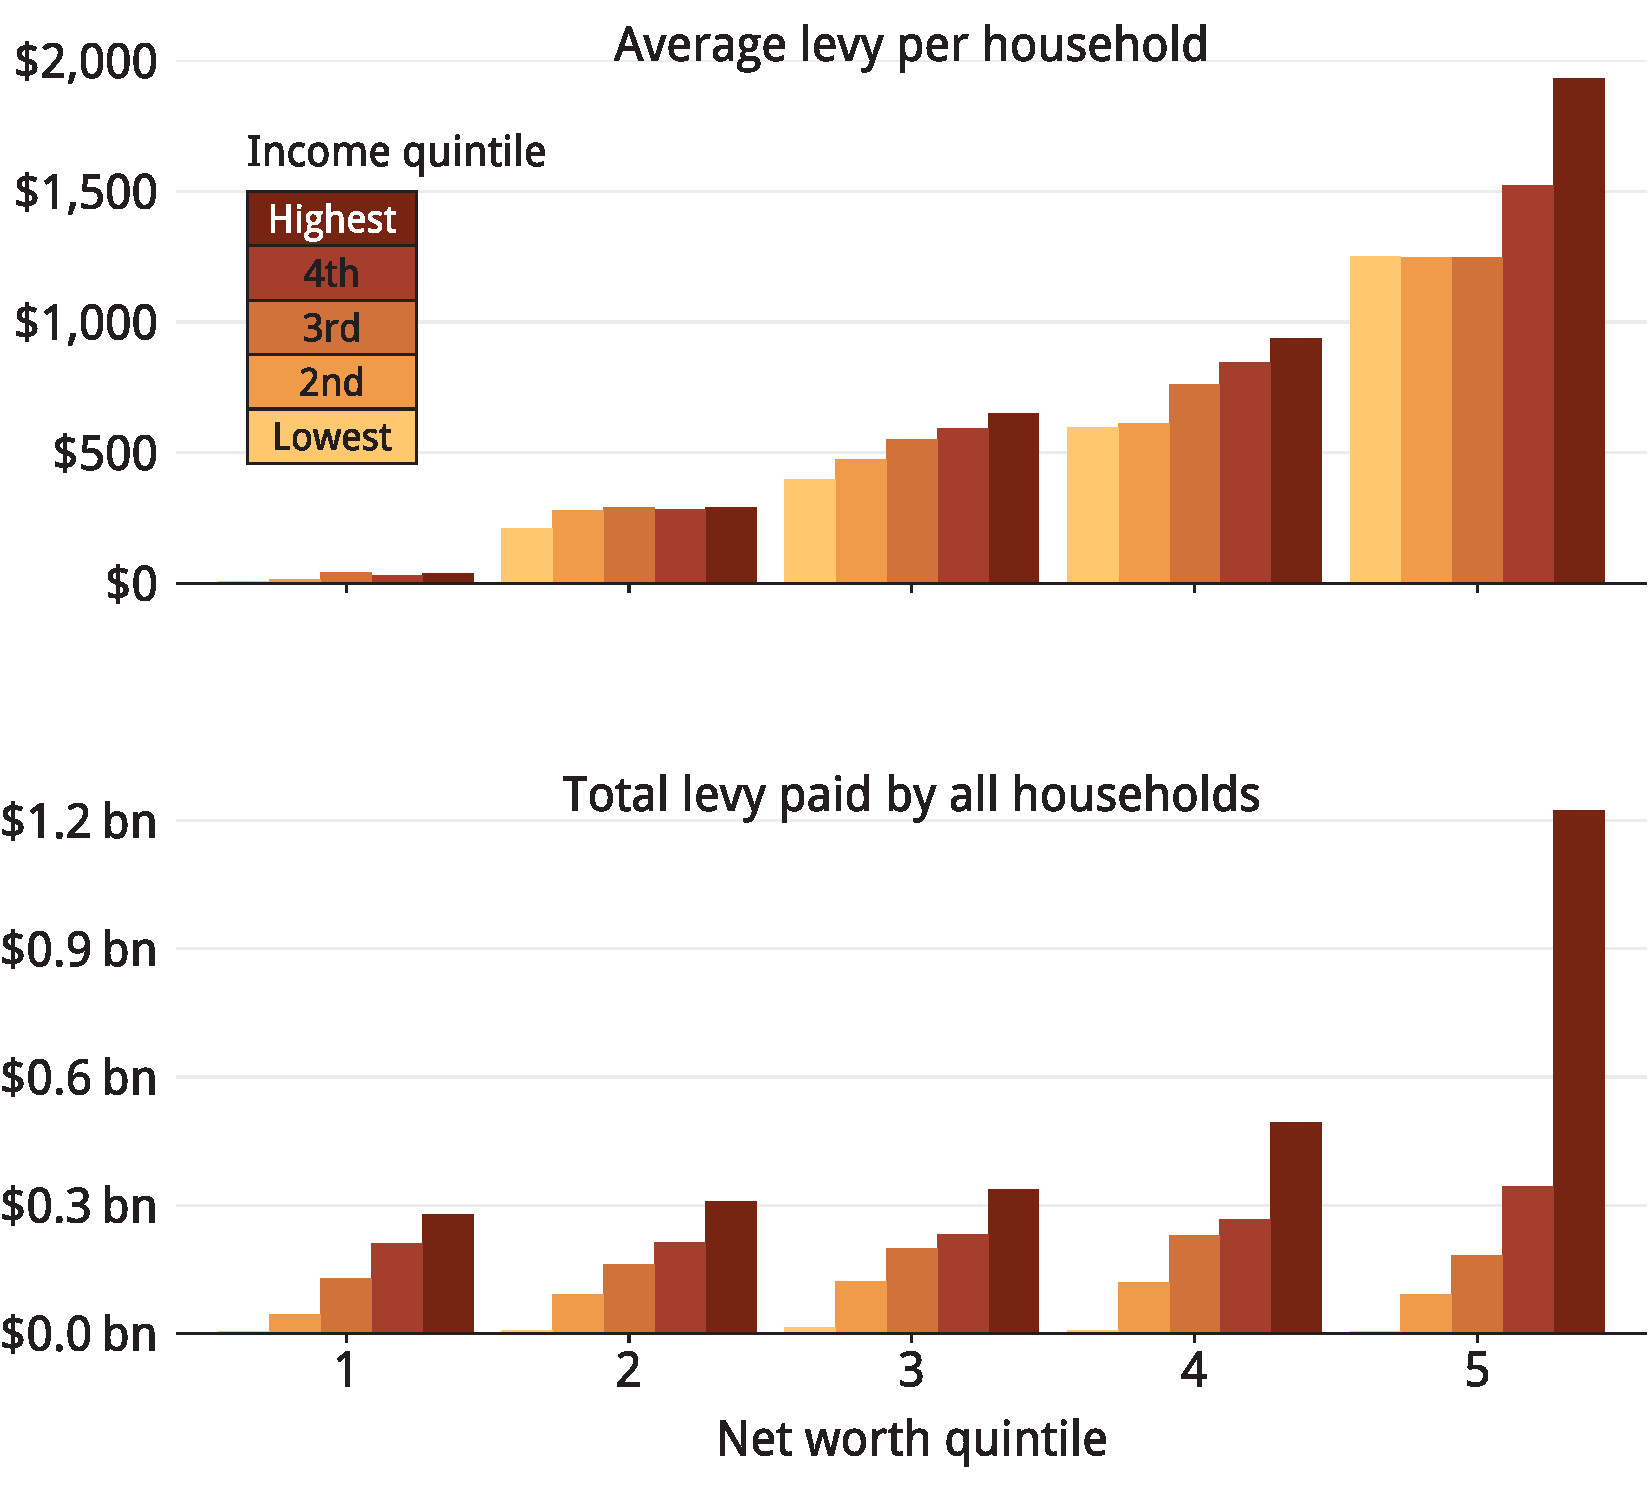
\includegraphics[width=11.000in,height=10in]{./Property-taxes/atlas/figure/PROP-Figure11-1} 

\end{knitrout}

\begin{knitrout}
\definecolor{shadecolor}{rgb}{0.969, 0.969, 0.969}\color{fgcolor}
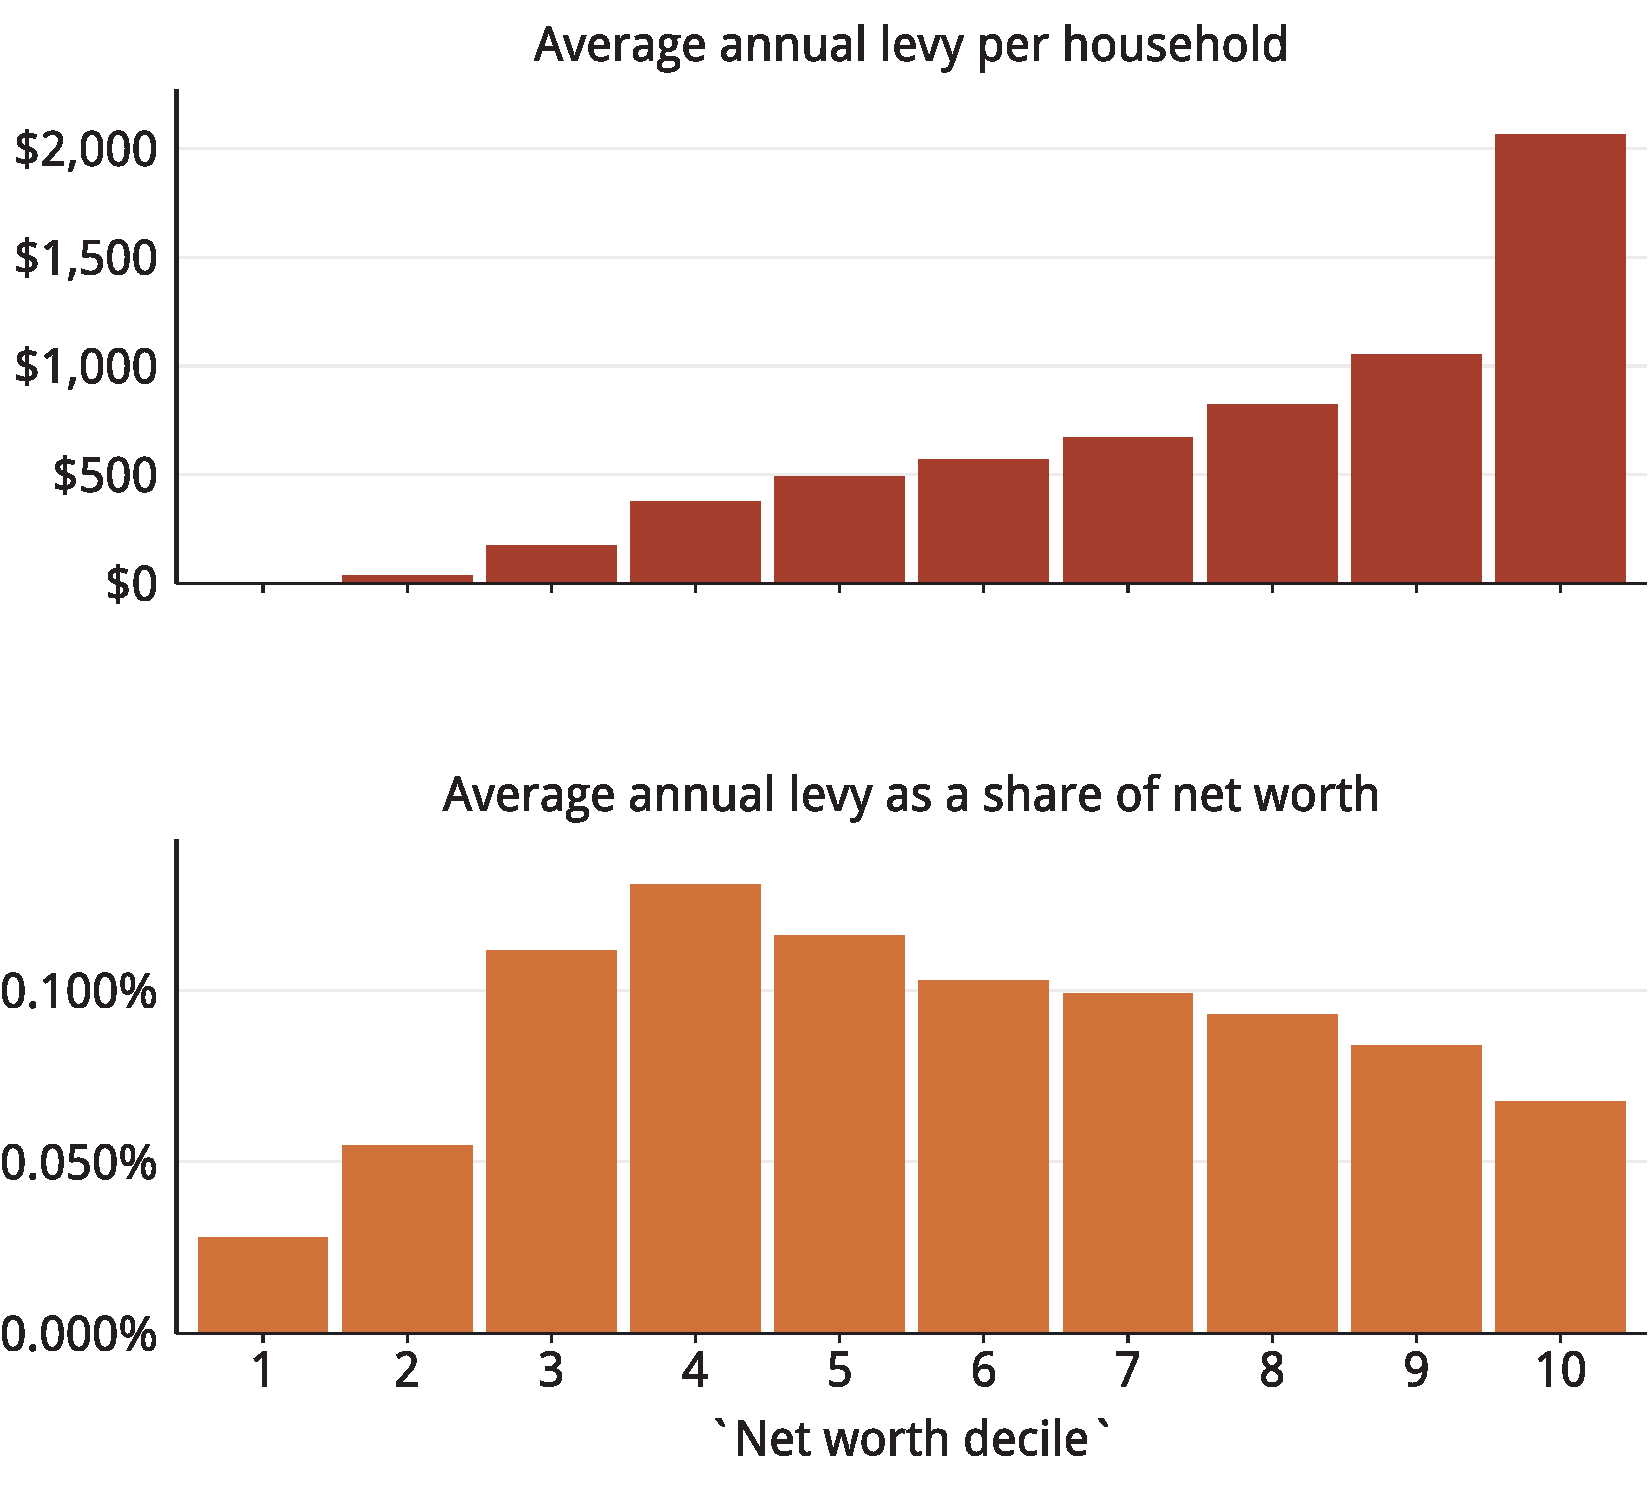
\includegraphics[width=11.000in,height=10in]{./Property-taxes/atlas/figure/PROP-Figure12-1} 

\end{knitrout}


% SUPER

\newpage
\begin{knitrout}
\definecolor{shadecolor}{rgb}{0.969, 0.969, 0.969}\color{fgcolor}\begin{kframe}


{\ttfamily\noindent\bfseries\color{errorcolor}{\#\# Error: `path` does not exist: './Super-tax-targeting/super-atlas/FIgure1-1.xlsx'}}\end{kframe}
\end{knitrout}

\begin{knitrout}
\definecolor{shadecolor}{rgb}{0.969, 0.969, 0.969}\color{fgcolor}
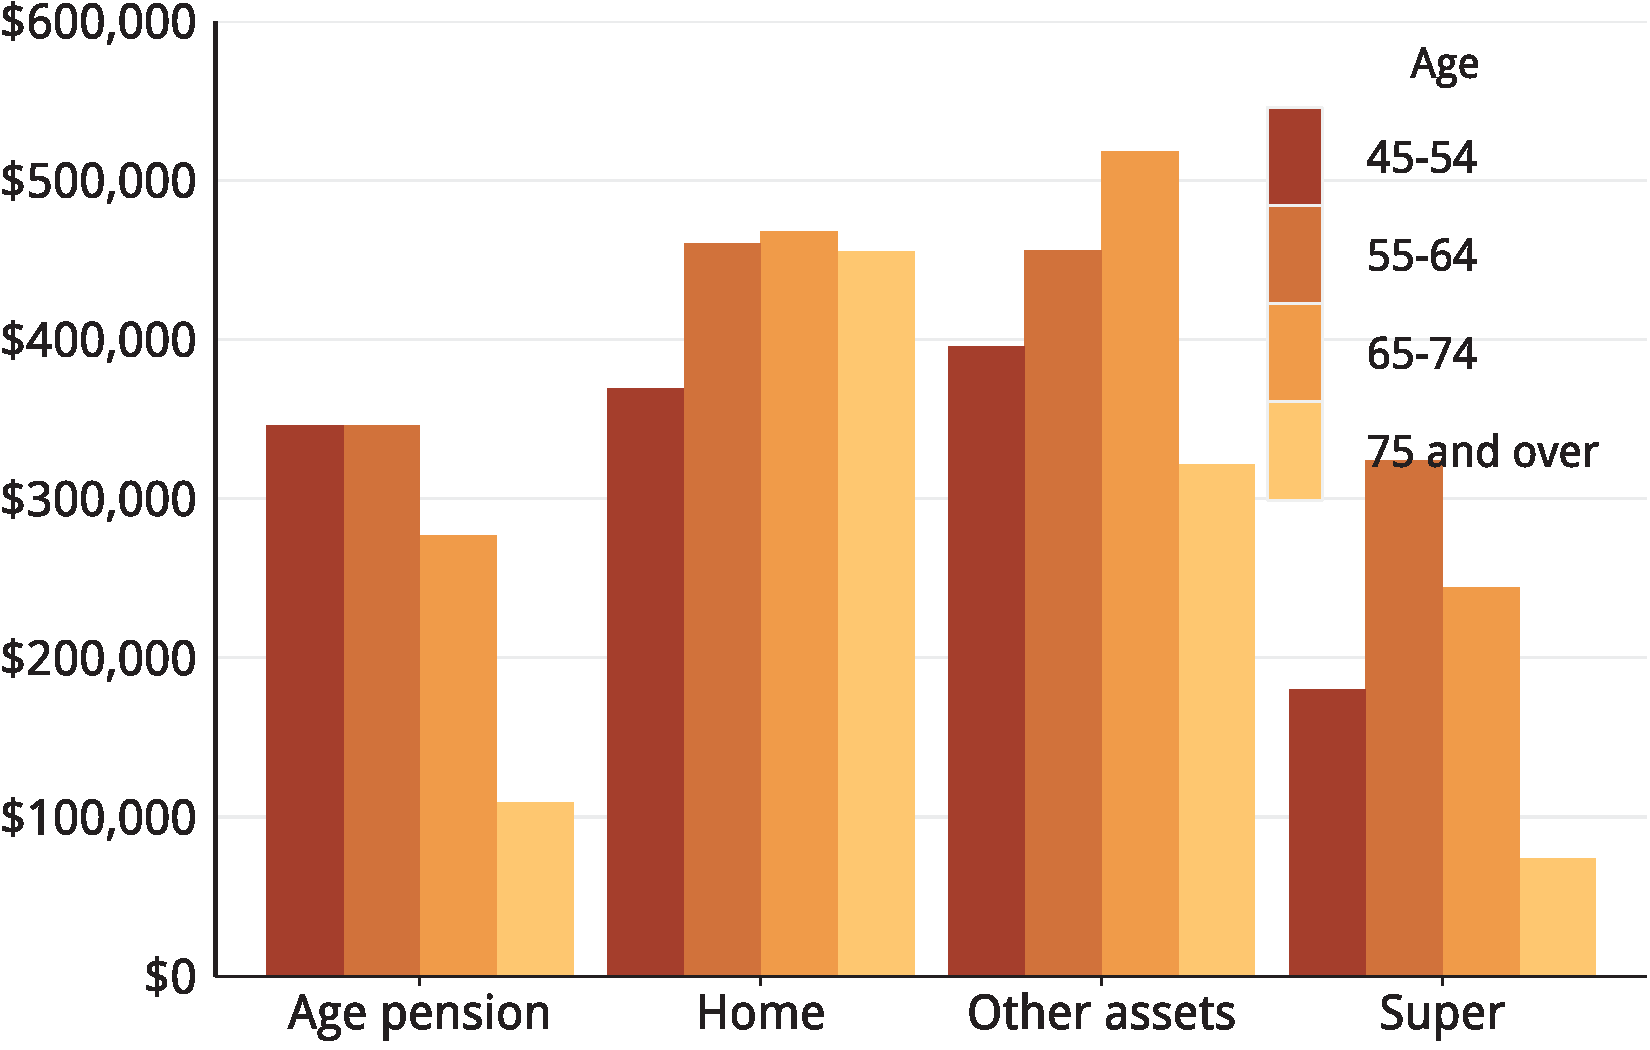
\includegraphics[width=11.000in,height=7.00in]{./Super-tax-targeting/b5-super-atlas/Figure2-1-1} 

\end{knitrout}

\begin{knitrout}
\definecolor{shadecolor}{rgb}{0.969, 0.969, 0.969}\color{fgcolor}
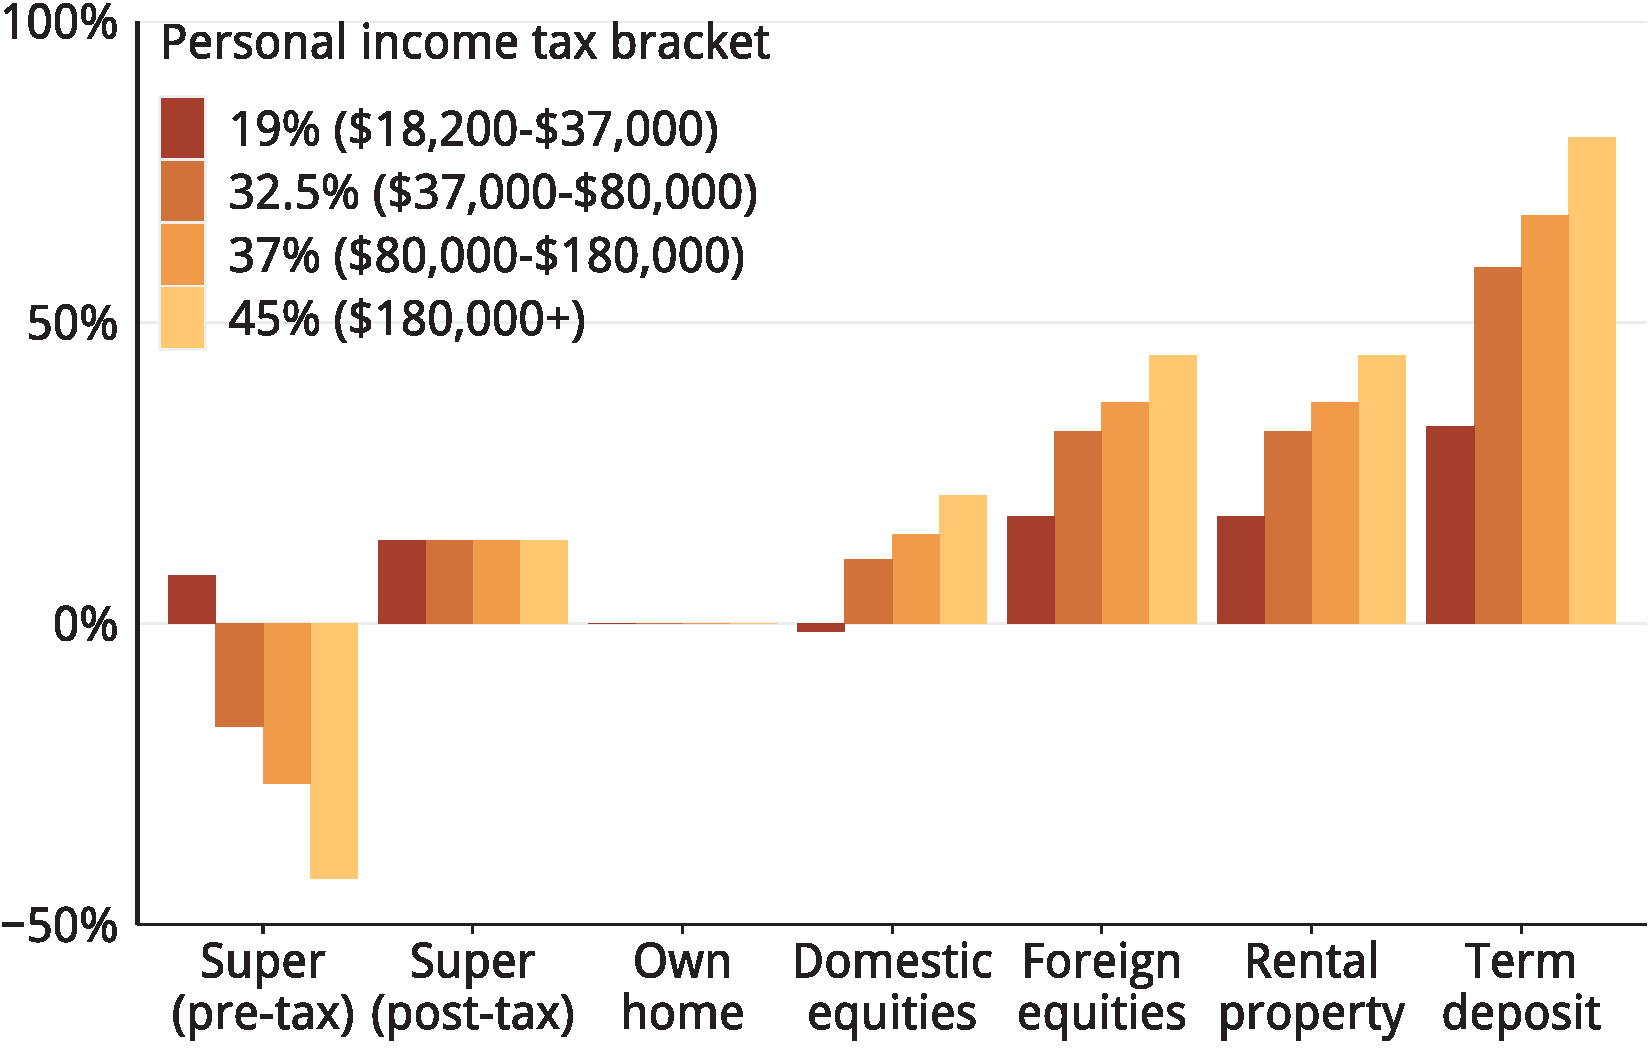
\includegraphics[width=11.000in,height=7.00in]{./Super-tax-targeting/b5-super-atlas/Figure2-3-1} 

\end{knitrout}

\begin{knitrout}
\definecolor{shadecolor}{rgb}{0.969, 0.969, 0.969}\color{fgcolor}
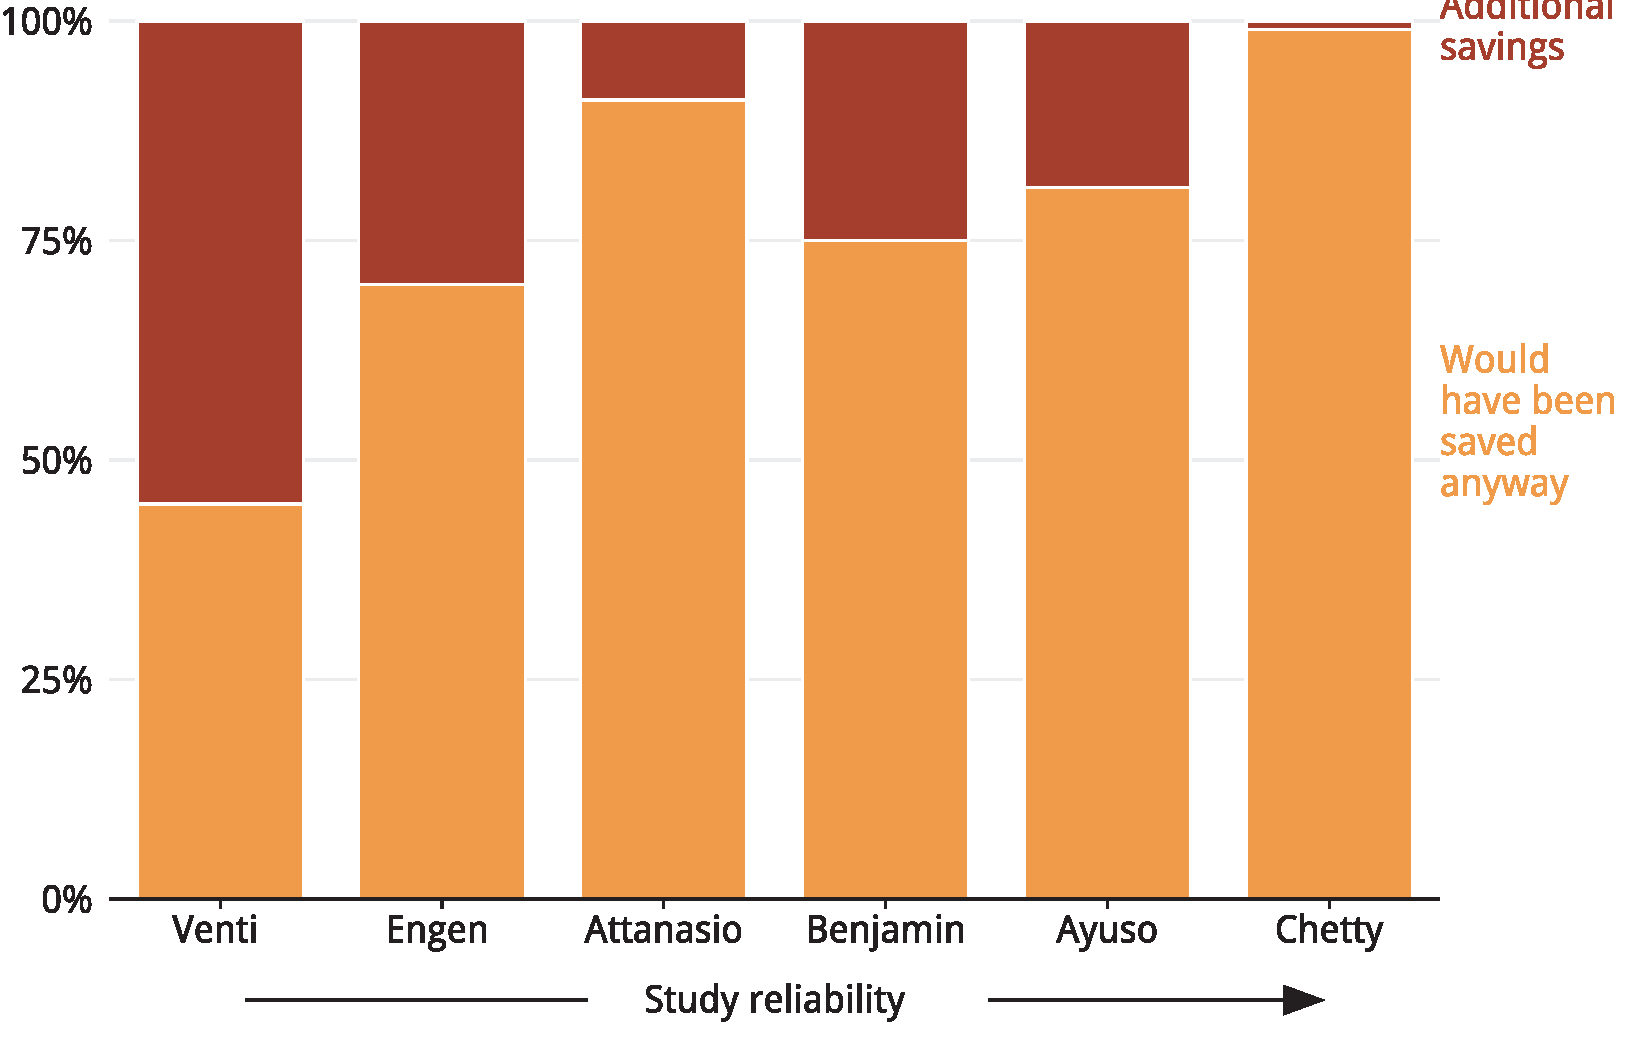
\includegraphics[width=11.000in,height=7.00in]{./Super-tax-targeting/b5-super-atlas/Figure2-4-1} 

\end{knitrout}

\begin{knitrout}
\definecolor{shadecolor}{rgb}{0.969, 0.969, 0.969}\color{fgcolor}
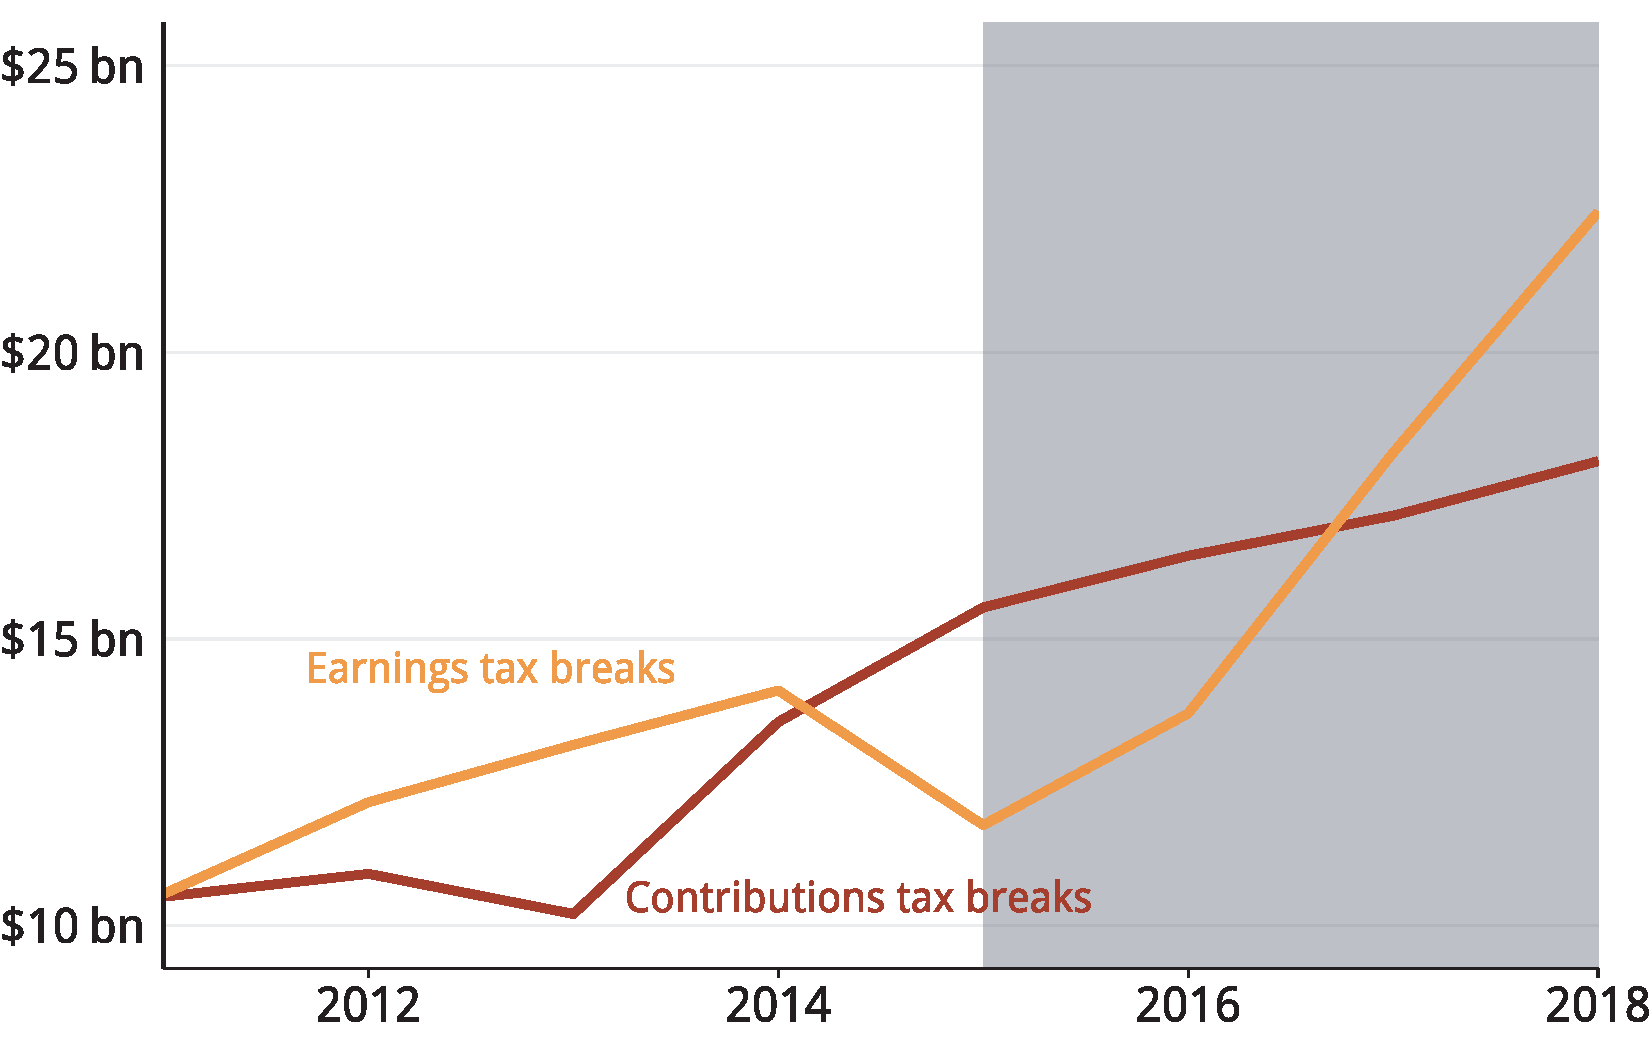
\includegraphics[width=11.000in,height=7.00in]{./Super-tax-targeting/b5-super-atlas/Figure2-5-1} 

\end{knitrout}

\begin{knitrout}
\definecolor{shadecolor}{rgb}{0.969, 0.969, 0.969}\color{fgcolor}
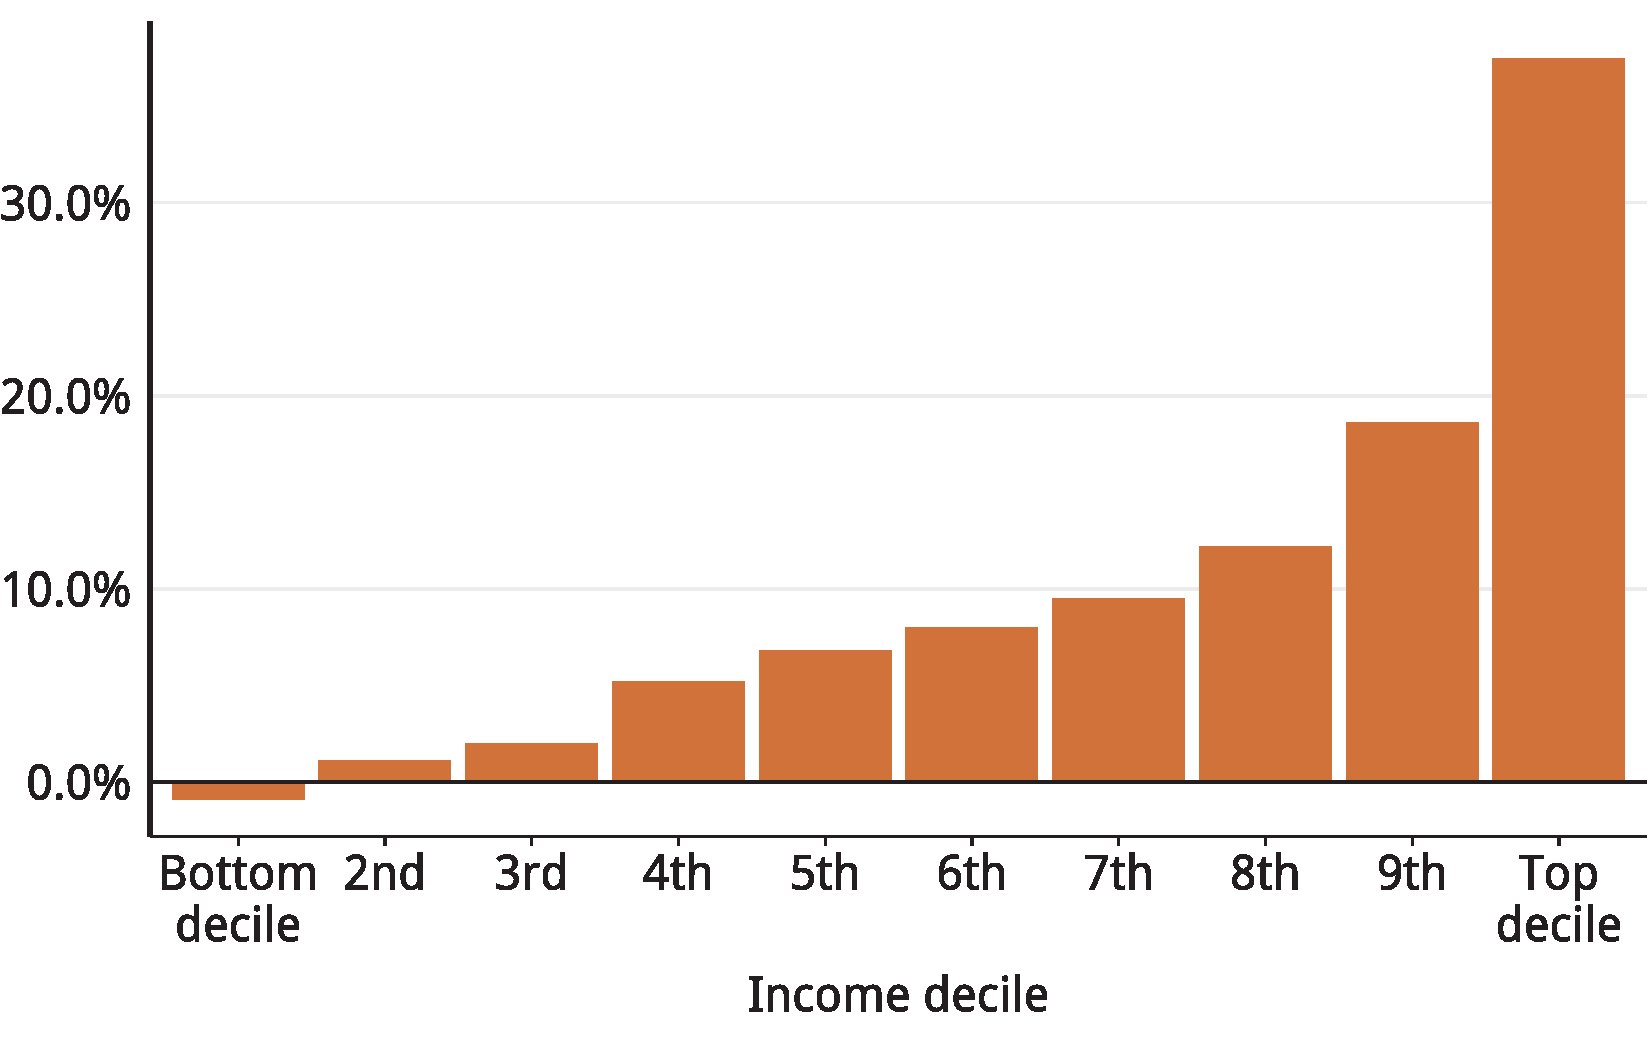
\includegraphics[width=11.000in,height=7.00in]{./Super-tax-targeting/b5-super-atlas/Figure3-1-1} 

\end{knitrout}

\begin{knitrout}
\definecolor{shadecolor}{rgb}{0.969, 0.969, 0.969}\color{fgcolor}
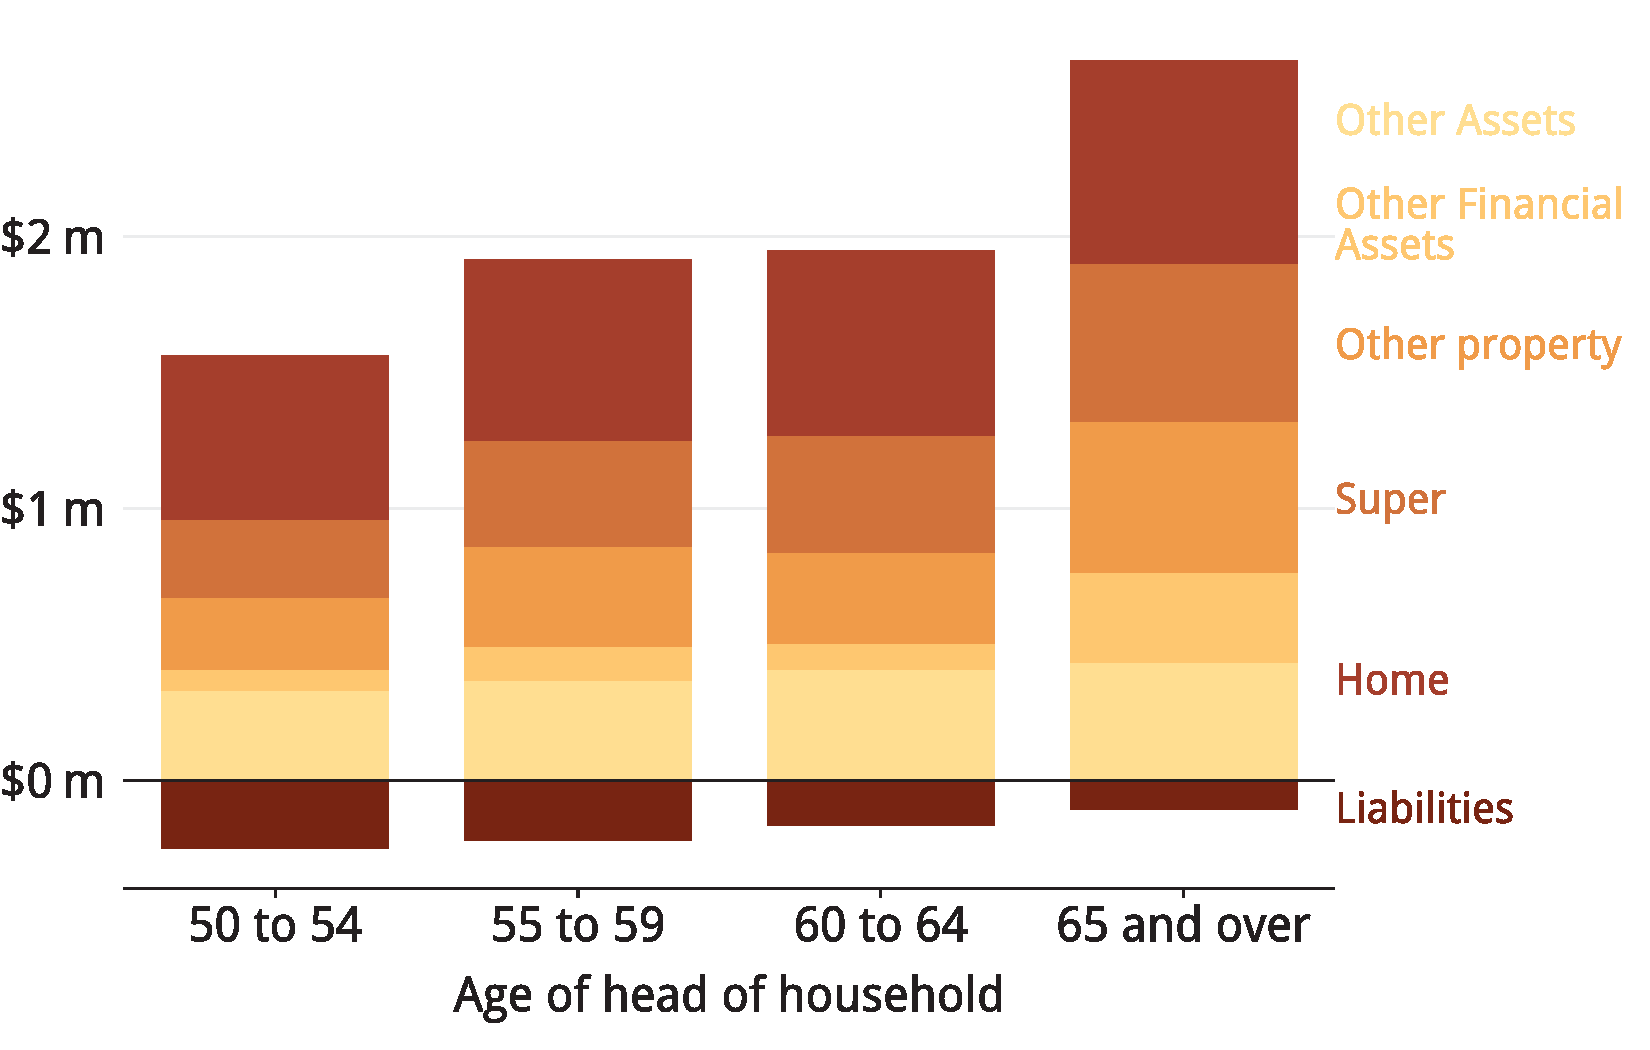
\includegraphics[width=11.000in,height=7.00in]{./Super-tax-targeting/b5-super-atlas/Figure3-2-1} 

\end{knitrout}

\begin{knitrout}
\definecolor{shadecolor}{rgb}{0.969, 0.969, 0.969}\color{fgcolor}
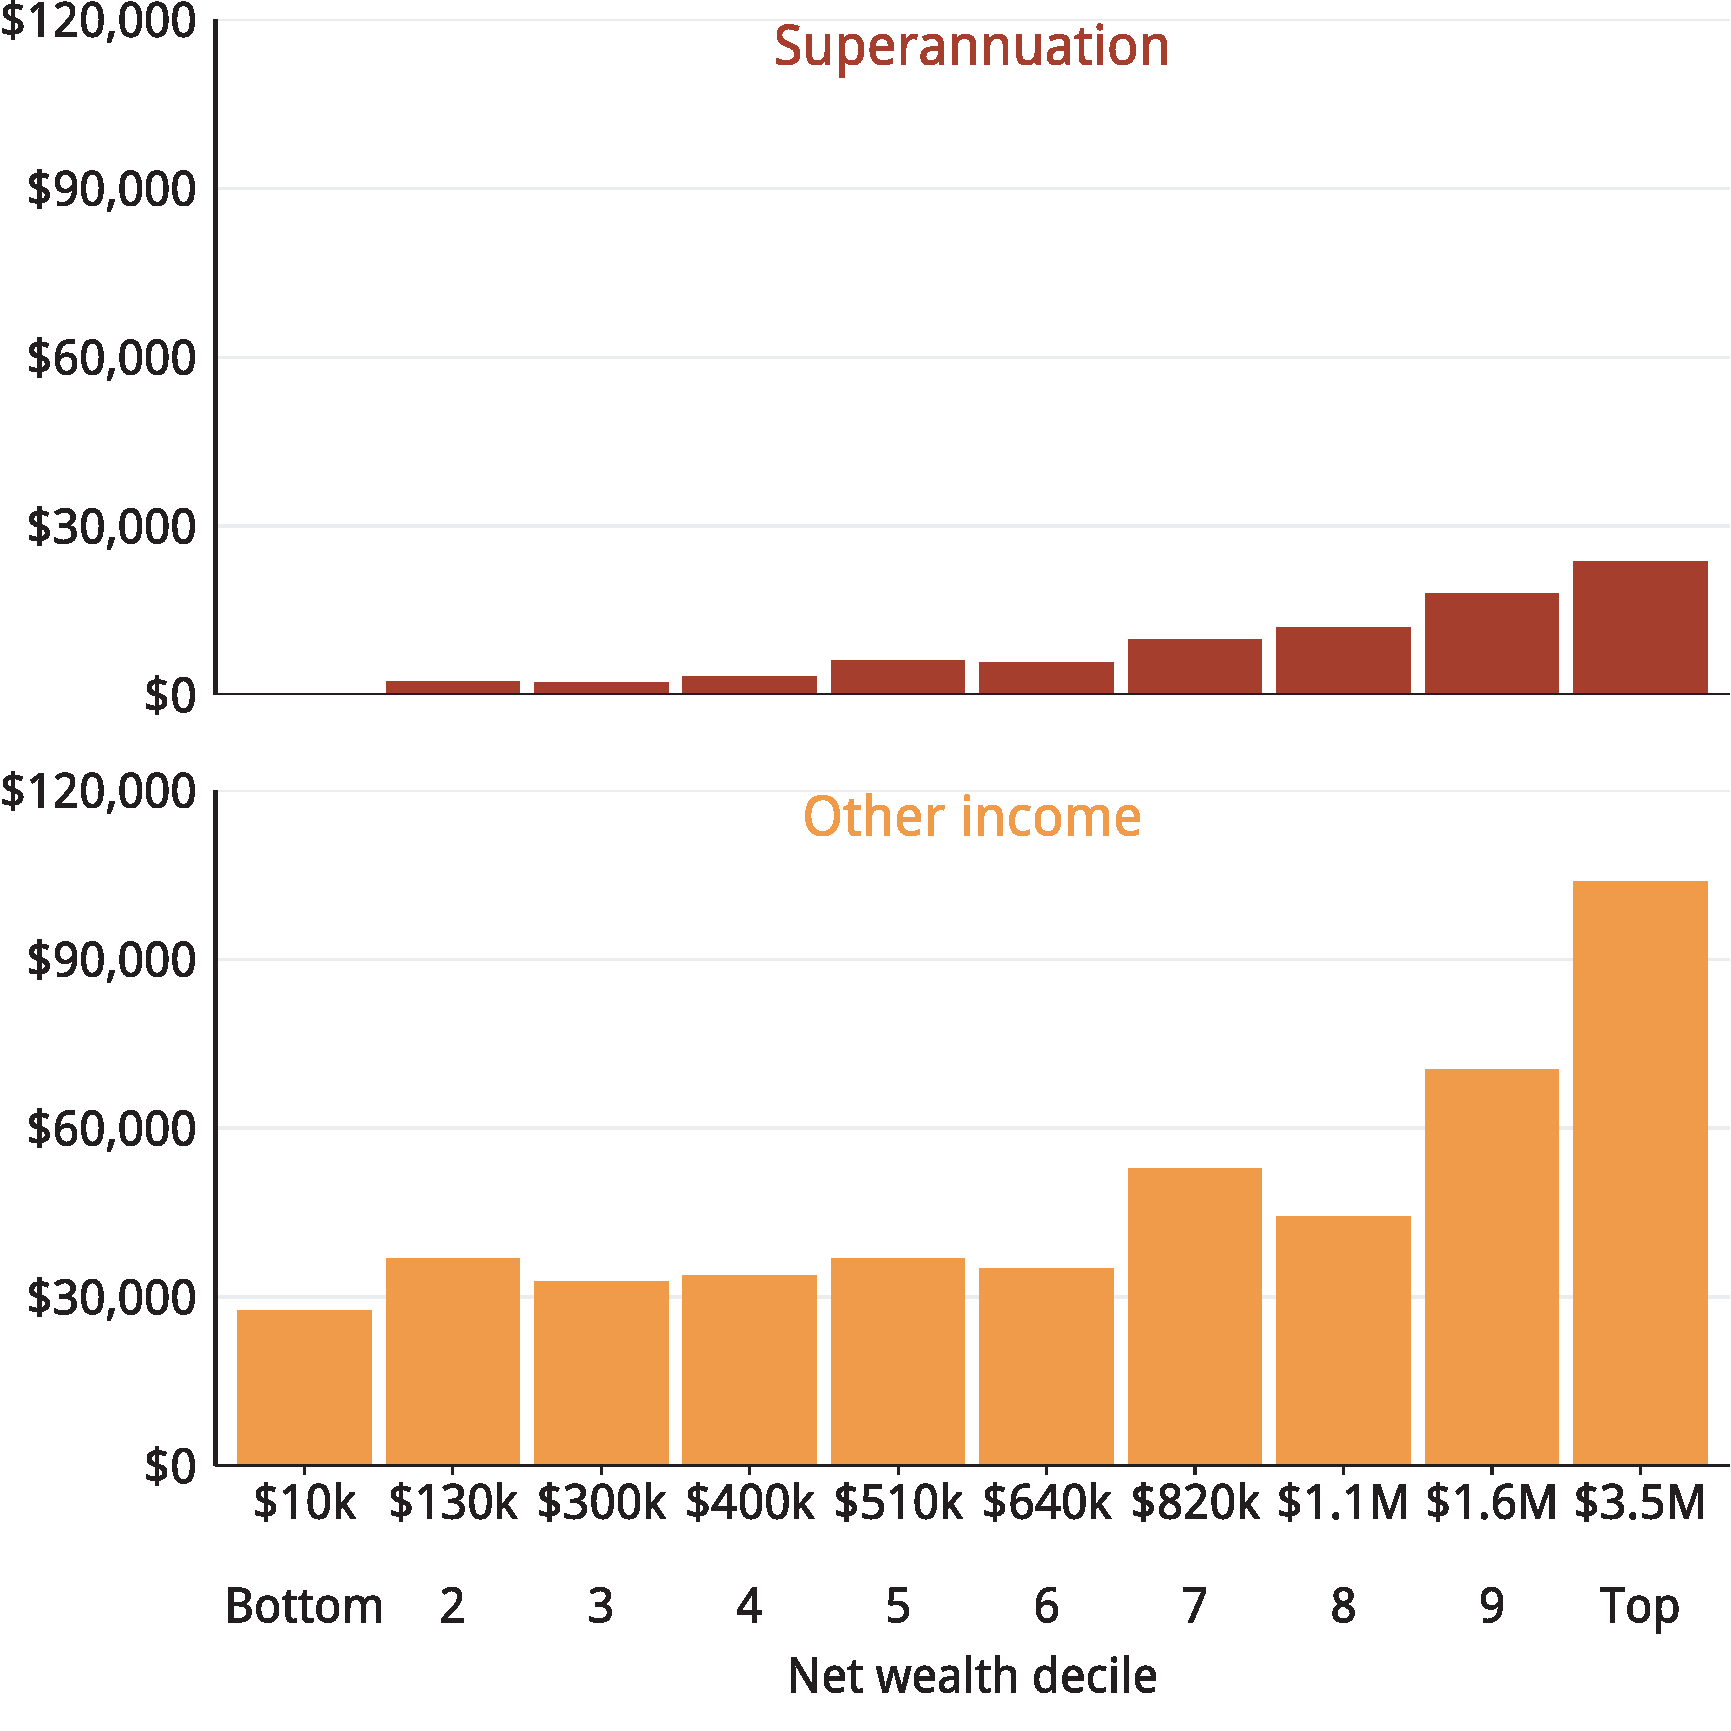
\includegraphics[width=11.55in,height=11.55in]{./Super-tax-targeting/b5-super-atlas/Figure3-3-1} 

\end{knitrout}

\begin{knitrout}
\definecolor{shadecolor}{rgb}{0.969, 0.969, 0.969}\color{fgcolor}
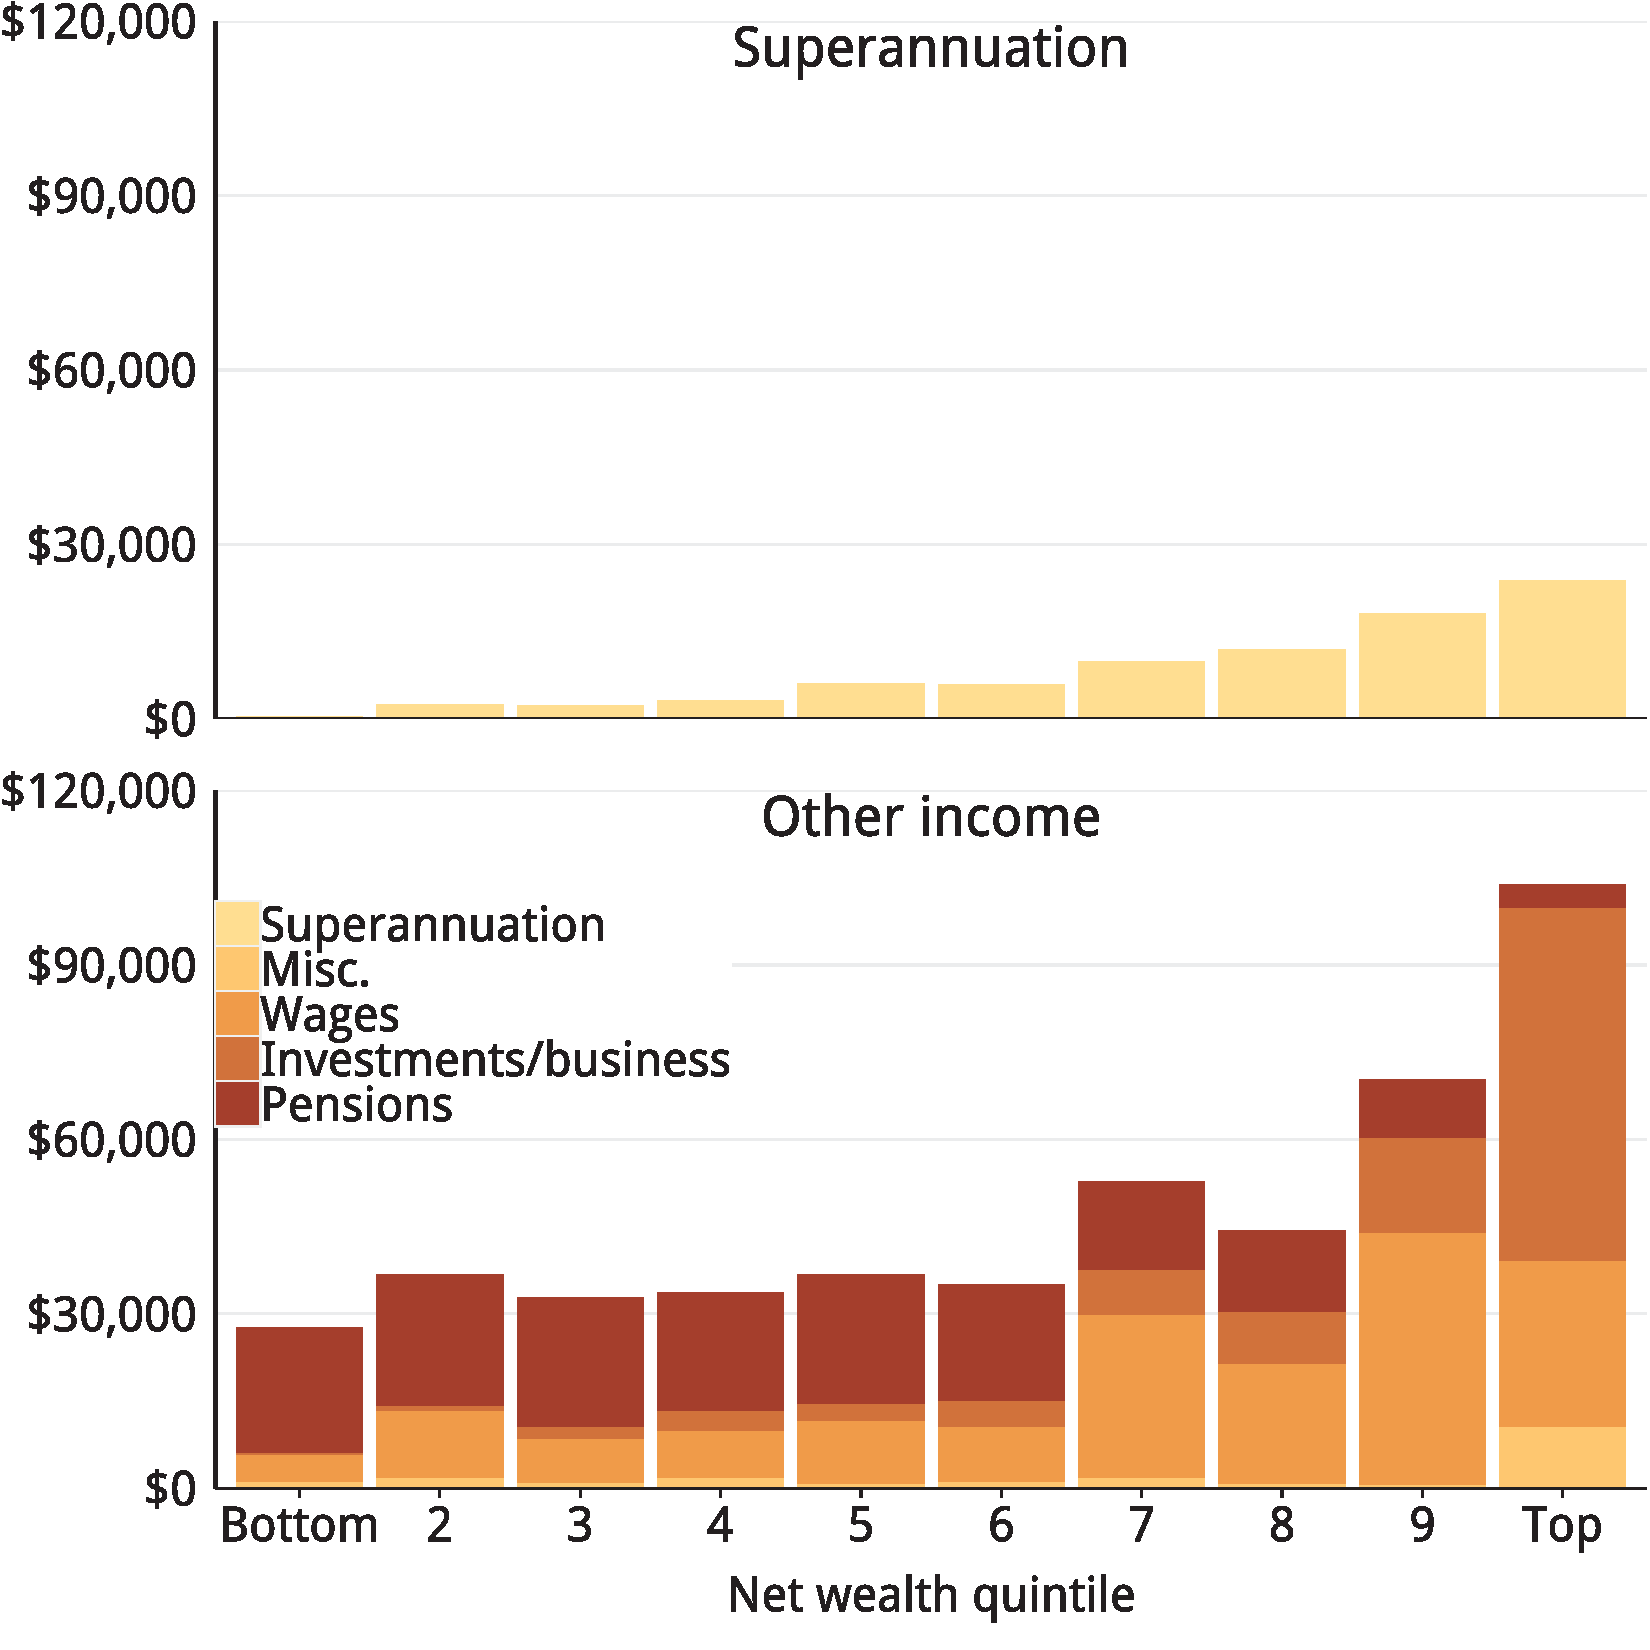
\includegraphics[width=11.000in,height=11in]{./Super-tax-targeting/b5-super-atlas/Figure3-3-detailed-1} 

\end{knitrout}

\begin{knitrout}
\definecolor{shadecolor}{rgb}{0.969, 0.969, 0.969}\color{fgcolor}
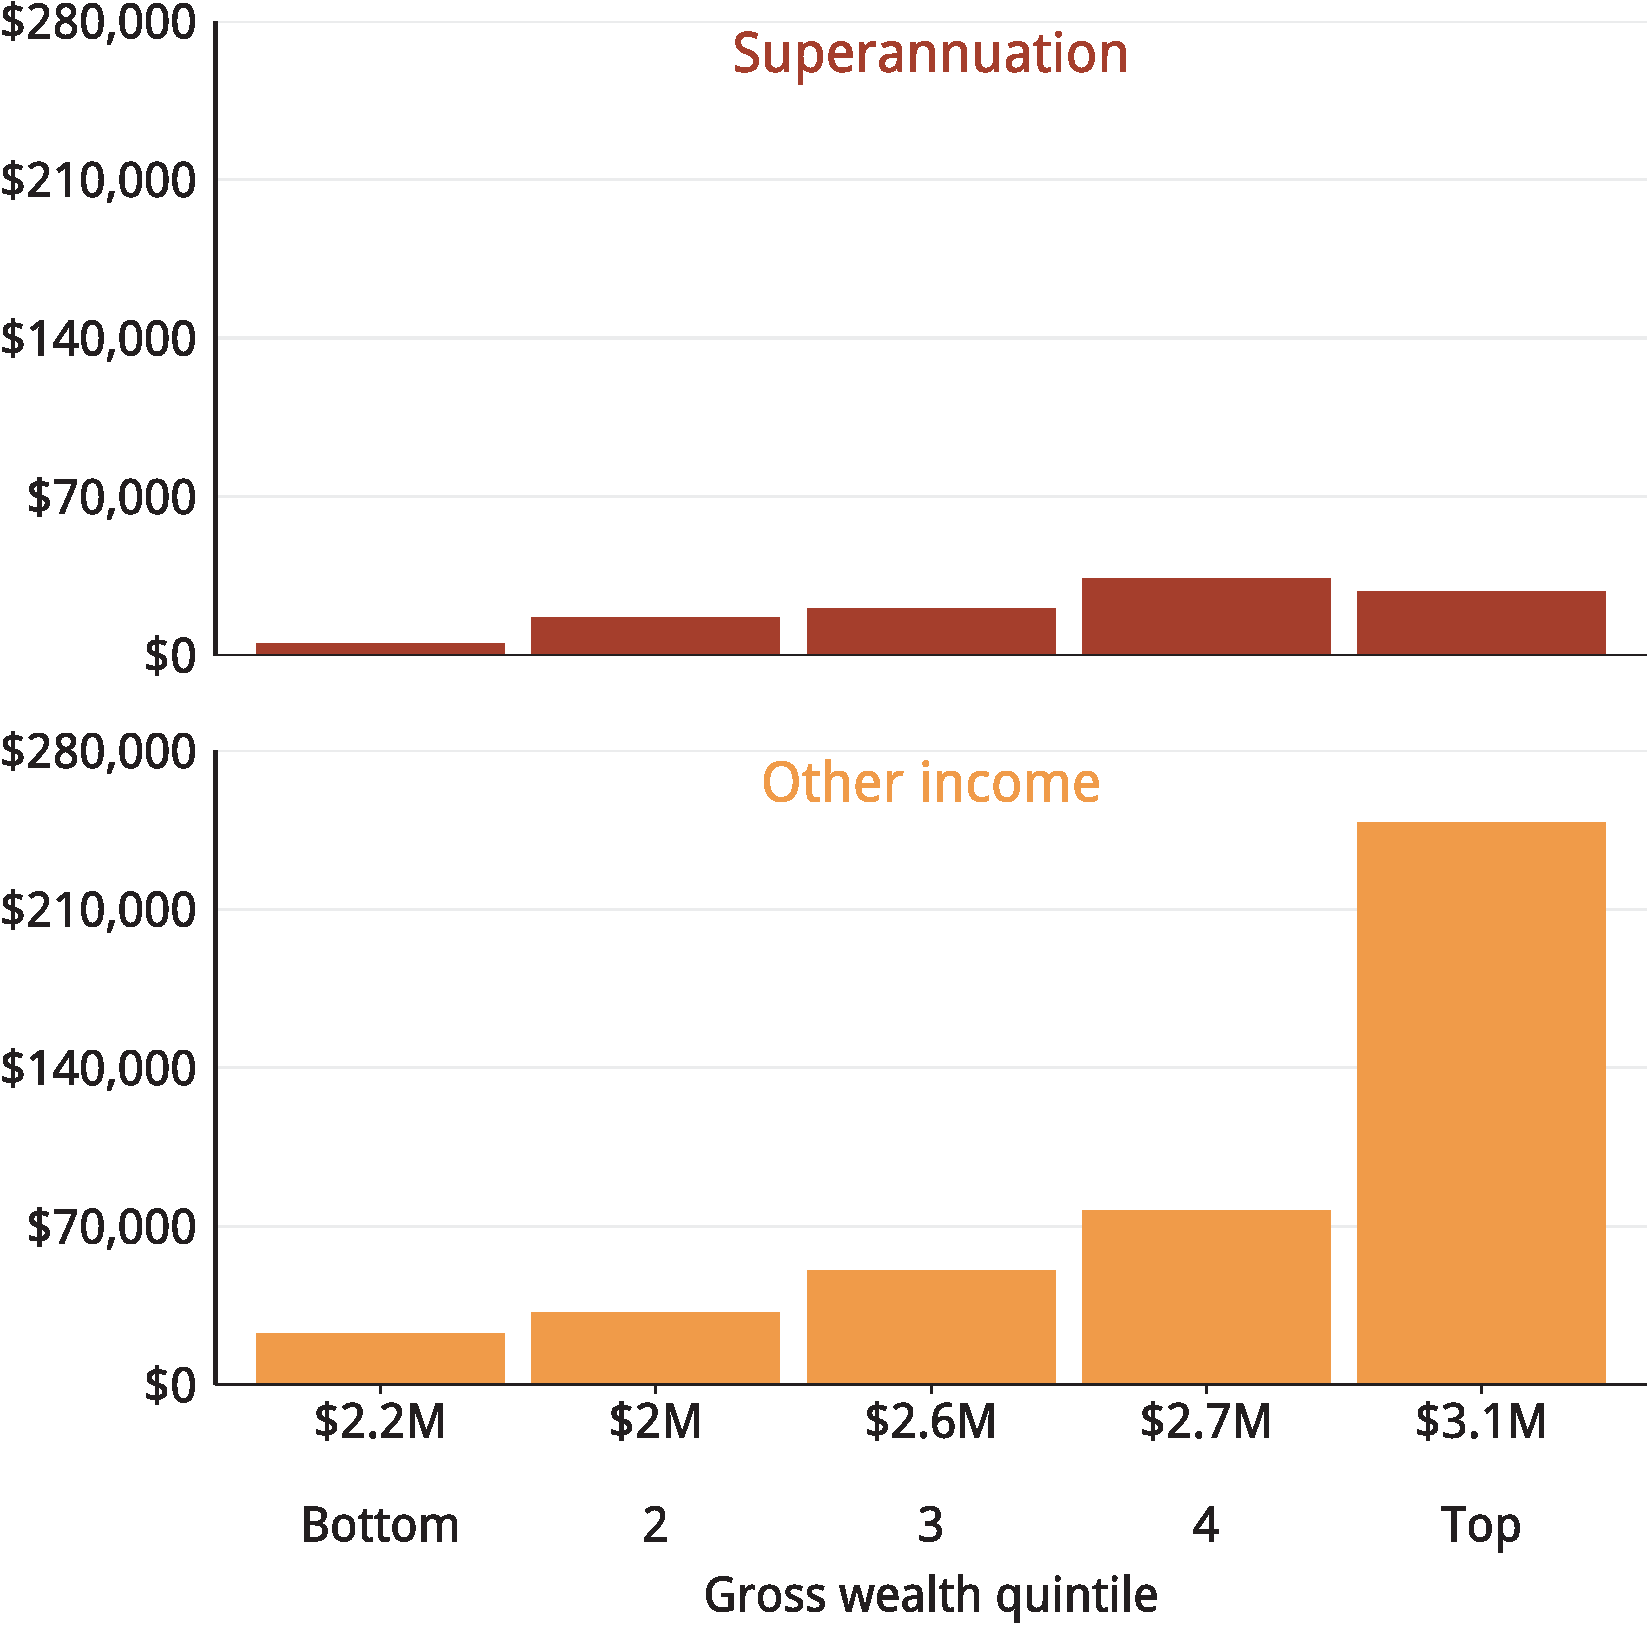
\includegraphics[width=11.000in,height=11in]{./Super-tax-targeting/b5-super-atlas/Figure3-4-1} 

\end{knitrout}

\begin{knitrout}
\definecolor{shadecolor}{rgb}{0.969, 0.969, 0.969}\color{fgcolor}\begin{kframe}


{\ttfamily\noindent\bfseries\color{errorcolor}{\#\# Error: `path` does not exist: './Super-tax-targeting/super-atlas/fig35.xlsx'}}

{\ttfamily\noindent\bfseries\color{errorcolor}{\#\# Error: `path` does not exist: './Super-tax-targeting/super-atlas/ASFA-retirement-standards.xlsx'}}

{\ttfamily\noindent\bfseries\color{errorcolor}{\#\# Error in eval(lhs, parent, parent): object 'fig35' not found}}\end{kframe}
\end{knitrout}

\begin{knitrout}
\definecolor{shadecolor}{rgb}{0.969, 0.969, 0.969}\color{fgcolor}\begin{kframe}


{\ttfamily\noindent\bfseries\color{errorcolor}{\#\# Error in eval(expr, envir, enclos): Unable to continue as the location of hes10bp.dta could not be found.\\\#\# I looked at 'D:/Github/Data/HES/hes10bp.dta'.}}

{\ttfamily\noindent\bfseries\color{errorcolor}{\#\# Error in read.dta("{}D:/Github/Data/HES/hes10bh.dta"{}): unable to open file: 'No such file or directory'}}

{\ttfamily\noindent\bfseries\color{errorcolor}{\#\# Error in eval(lhs, parent, parent): object 'hes10' not found}}

{\ttfamily\noindent\bfseries\color{errorcolor}{\#\# Error in eval(lhs, parent, parent): object 'hes10' not found}}

{\ttfamily\noindent\bfseries\color{errorcolor}{\#\# Error in dots\_values(...): object 'dat\_include\_housing' not found}}\end{kframe}
\end{knitrout}

\begin{knitrout}
\definecolor{shadecolor}{rgb}{0.969, 0.969, 0.969}\color{fgcolor}
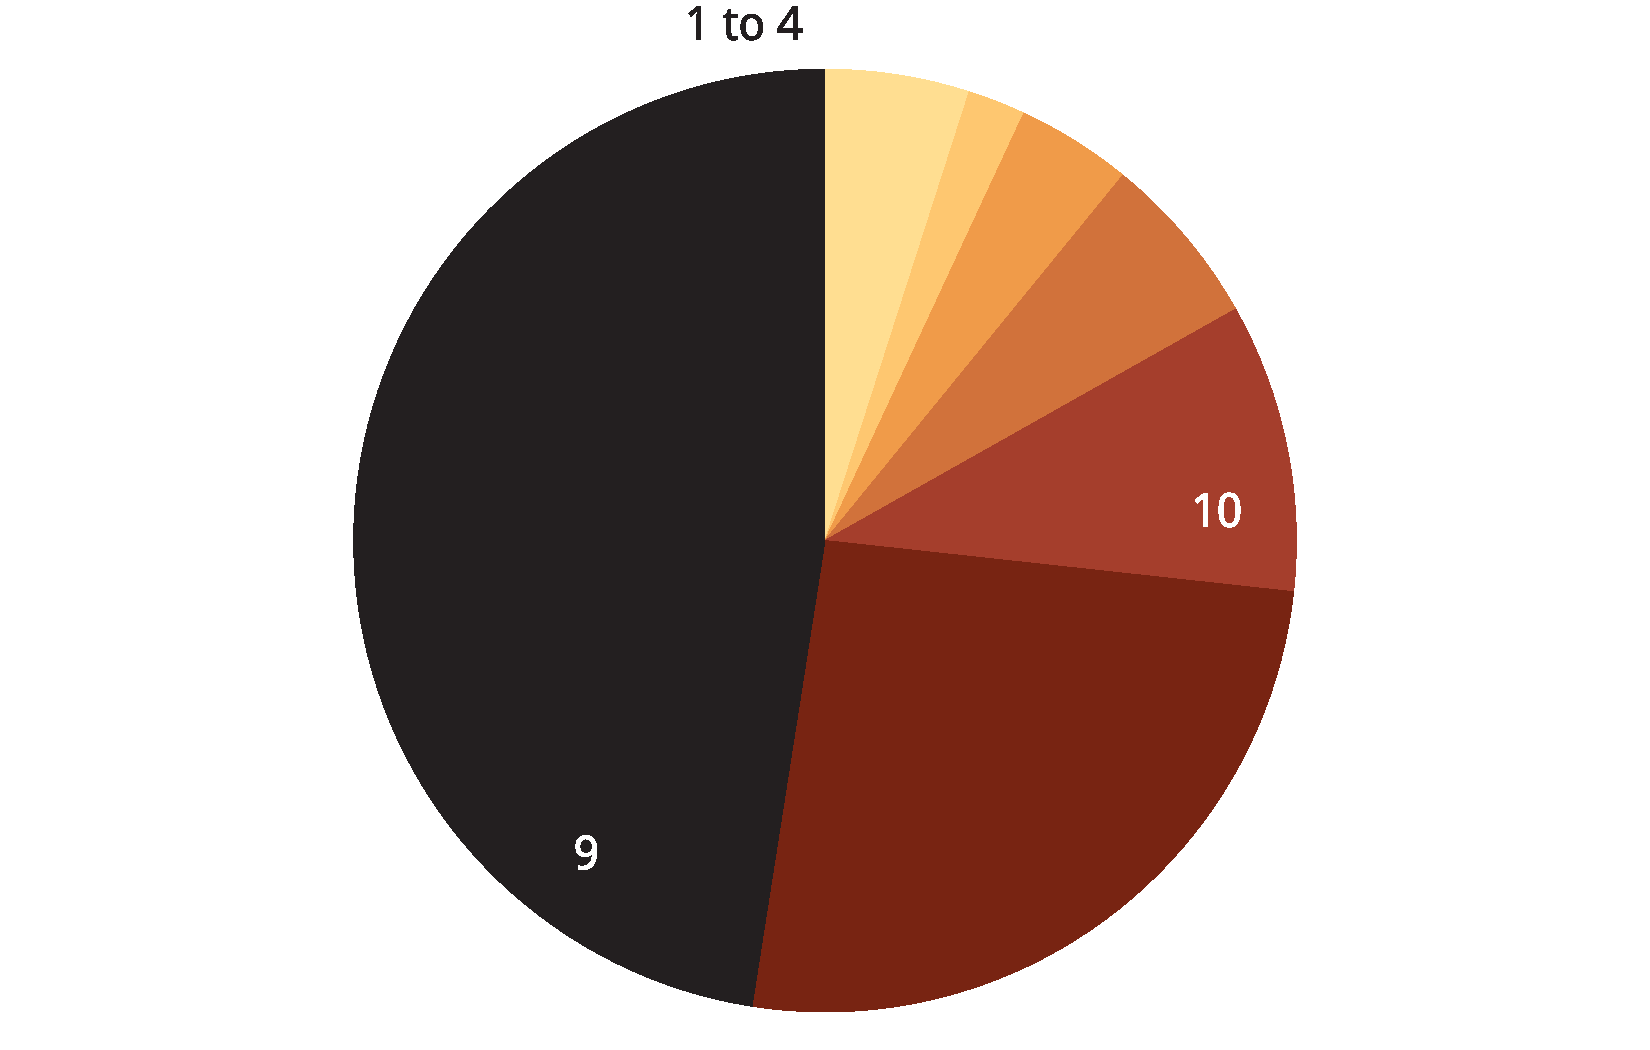
\includegraphics[width=11.000in,height=7.00in]{./Super-tax-targeting/b5-super-atlas/Figure3-7-1} 

\end{knitrout}

\begin{knitrout}
\definecolor{shadecolor}{rgb}{0.969, 0.969, 0.969}\color{fgcolor}
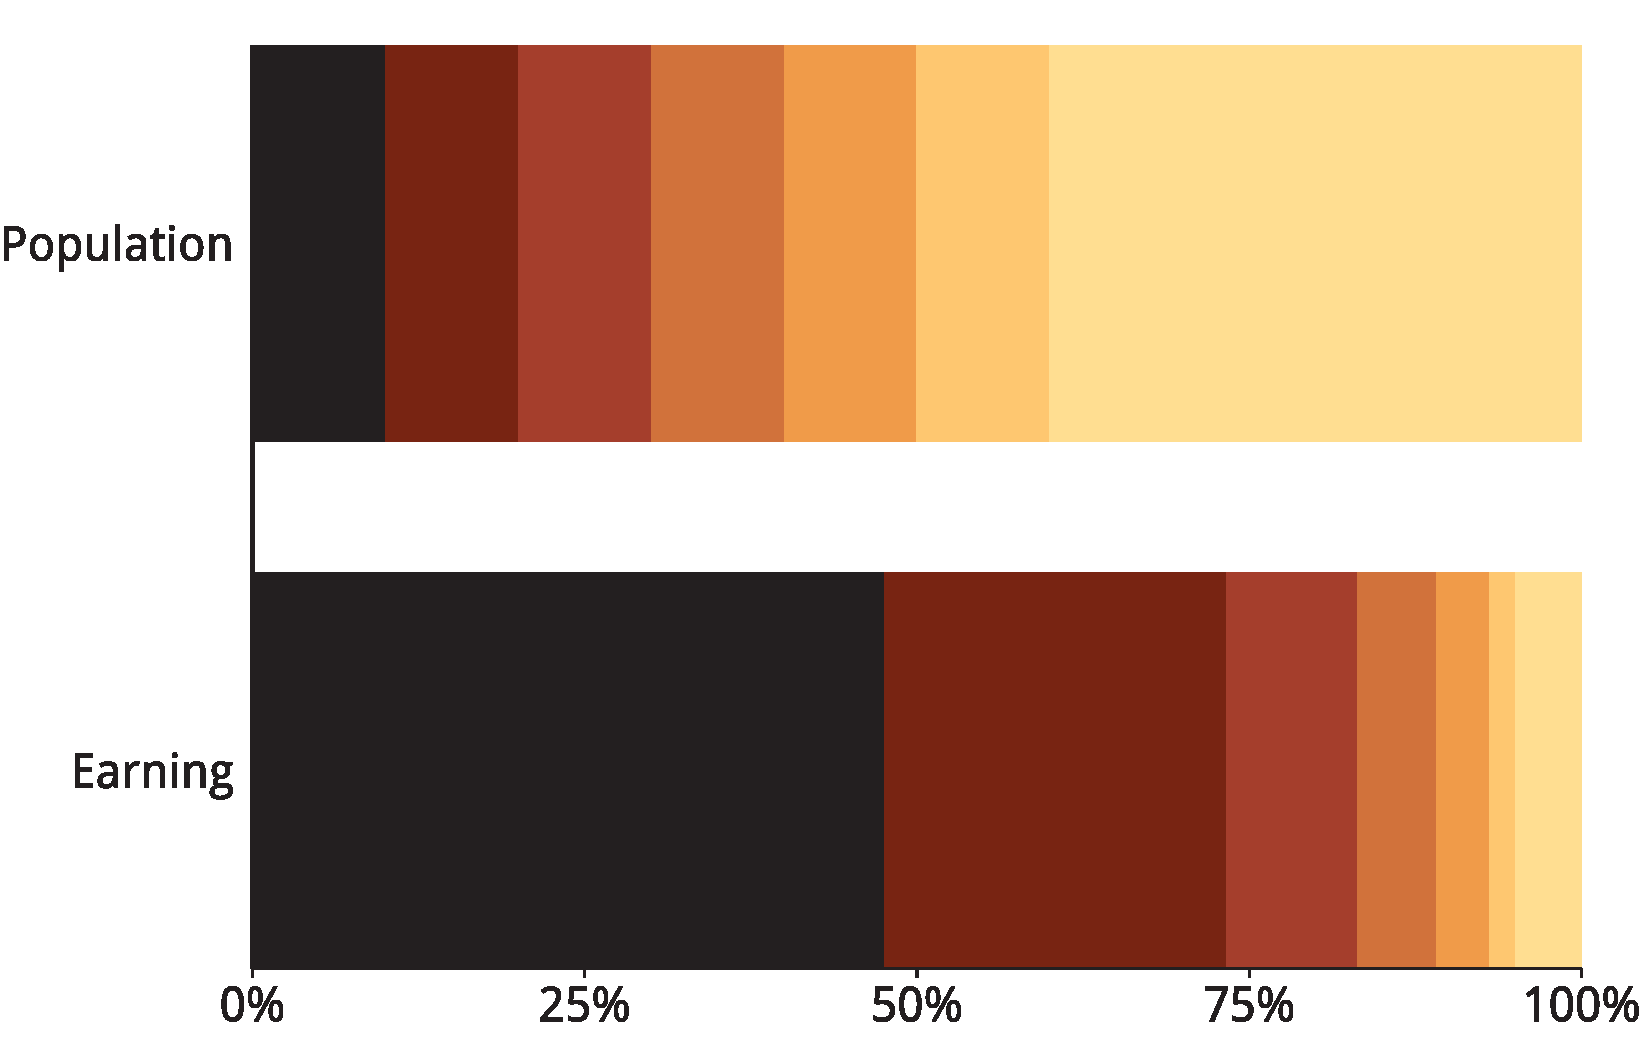
\includegraphics[width=11.000in,height=7.00in]{./Super-tax-targeting/b5-super-atlas/Figure3-7-bar-1} 

\end{knitrout}

\begin{knitrout}
\definecolor{shadecolor}{rgb}{0.969, 0.969, 0.969}\color{fgcolor}
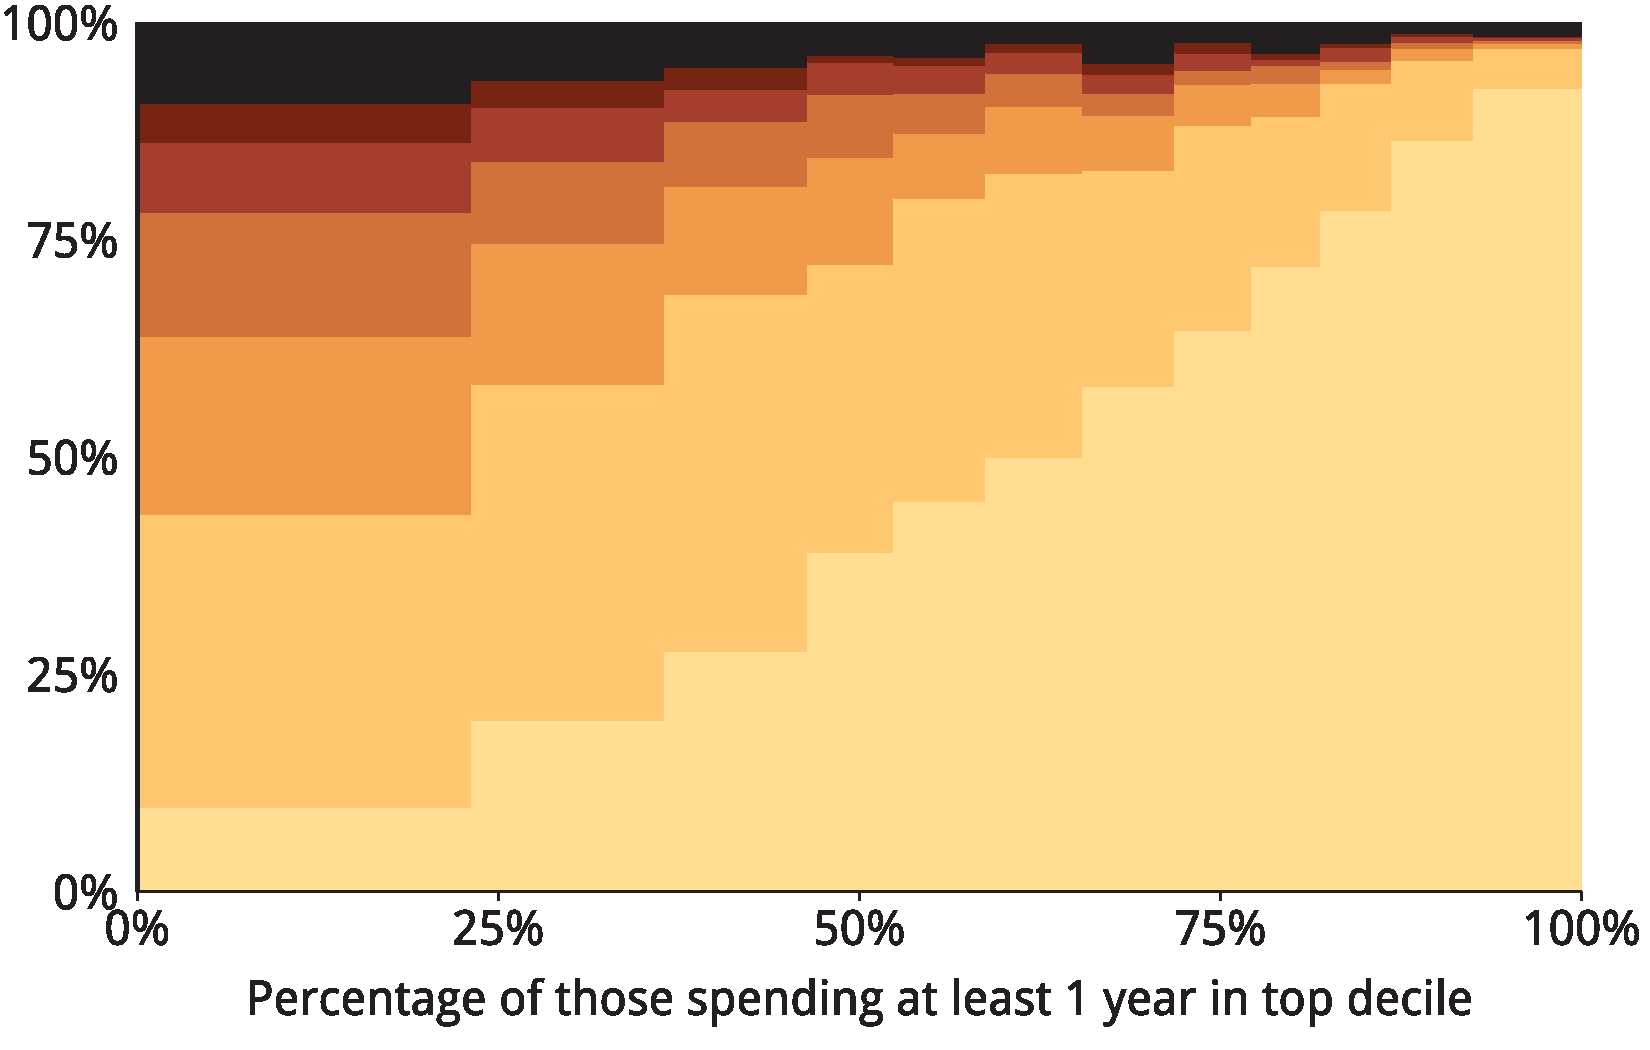
\includegraphics[width=11.000in,height=7.00in]{./Super-tax-targeting/b5-super-atlas/Figure3-8-marimekko-1} 

\end{knitrout}

\begin{knitrout}
\definecolor{shadecolor}{rgb}{0.969, 0.969, 0.969}\color{fgcolor}
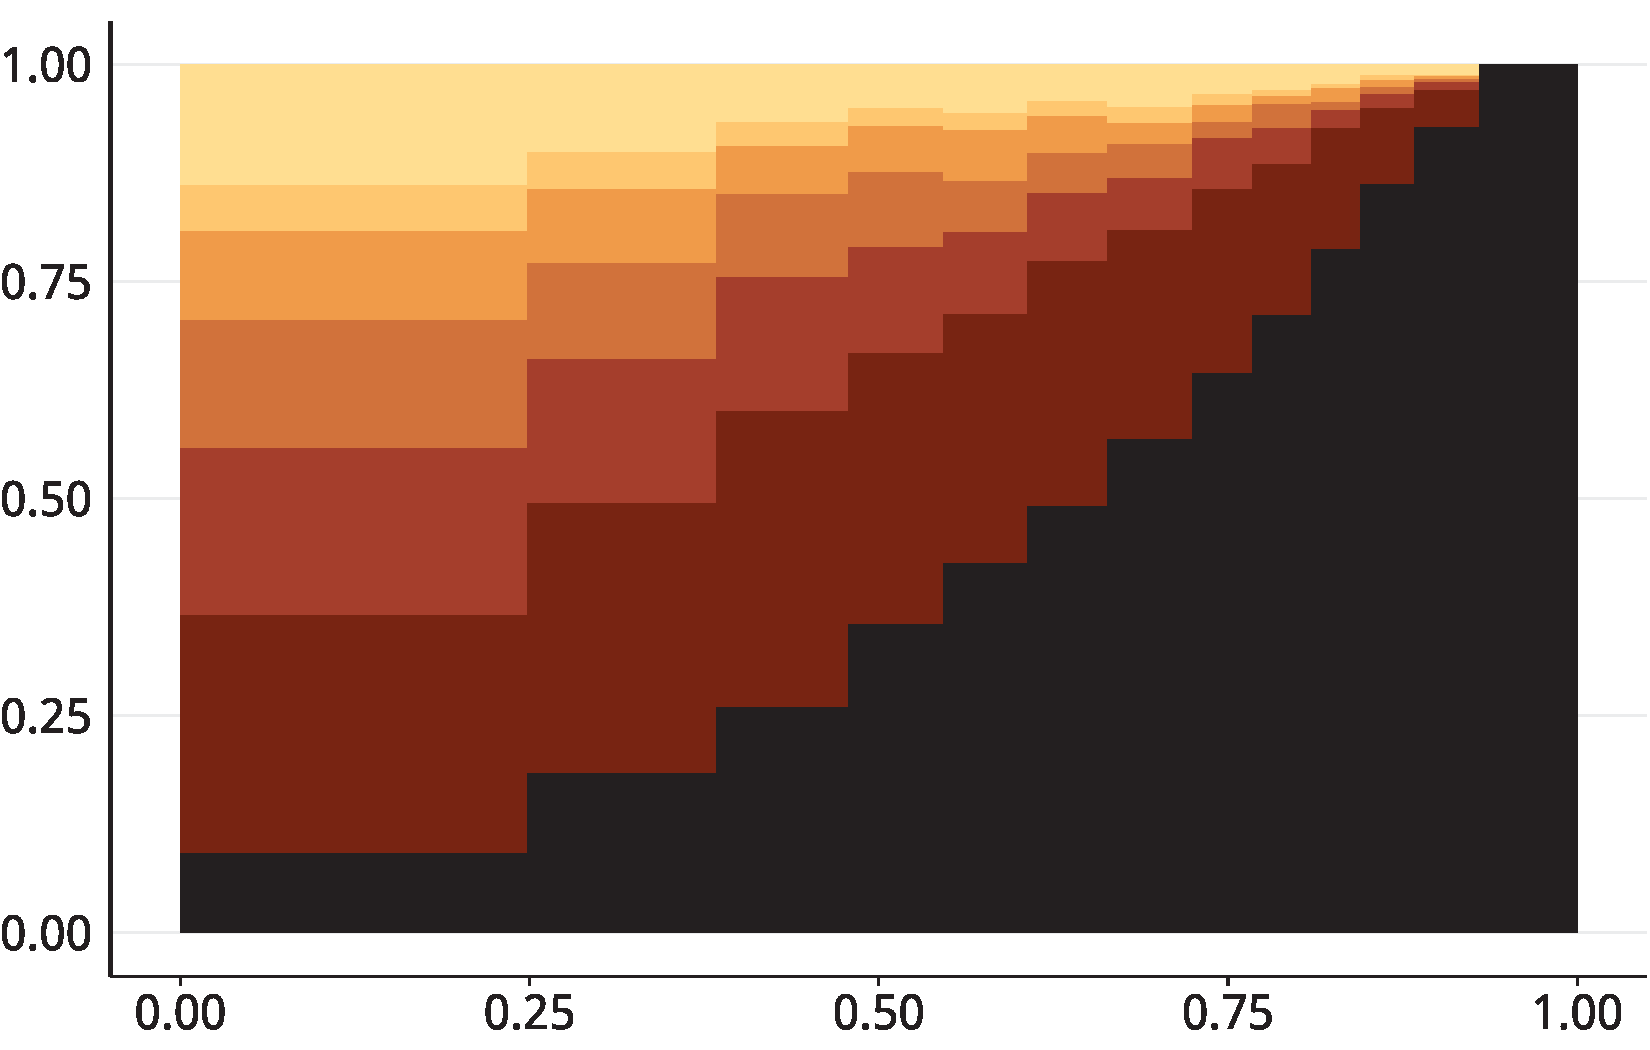
\includegraphics[width=11.000in,height=7.00in]{./Super-tax-targeting/b5-super-atlas/Figure3-8-1} 

\end{knitrout}

\begin{knitrout}
\definecolor{shadecolor}{rgb}{0.969, 0.969, 0.969}\color{fgcolor}\begin{kframe}


{\ttfamily\noindent\bfseries\color{errorcolor}{\#\# Error in UseMethod("{}validGrob"{}): no applicable method for 'validGrob' applied to an object of class "{}list"{}}}

{\ttfamily\noindent\bfseries\color{errorcolor}{\#\# Error in grid.Call(C\_convert, x, as.integer(whatfrom), as.integer(whatto), : invalid line end}}\end{kframe}
\end{knitrout}

\begin{knitrout}
\definecolor{shadecolor}{rgb}{0.969, 0.969, 0.969}\color{fgcolor}
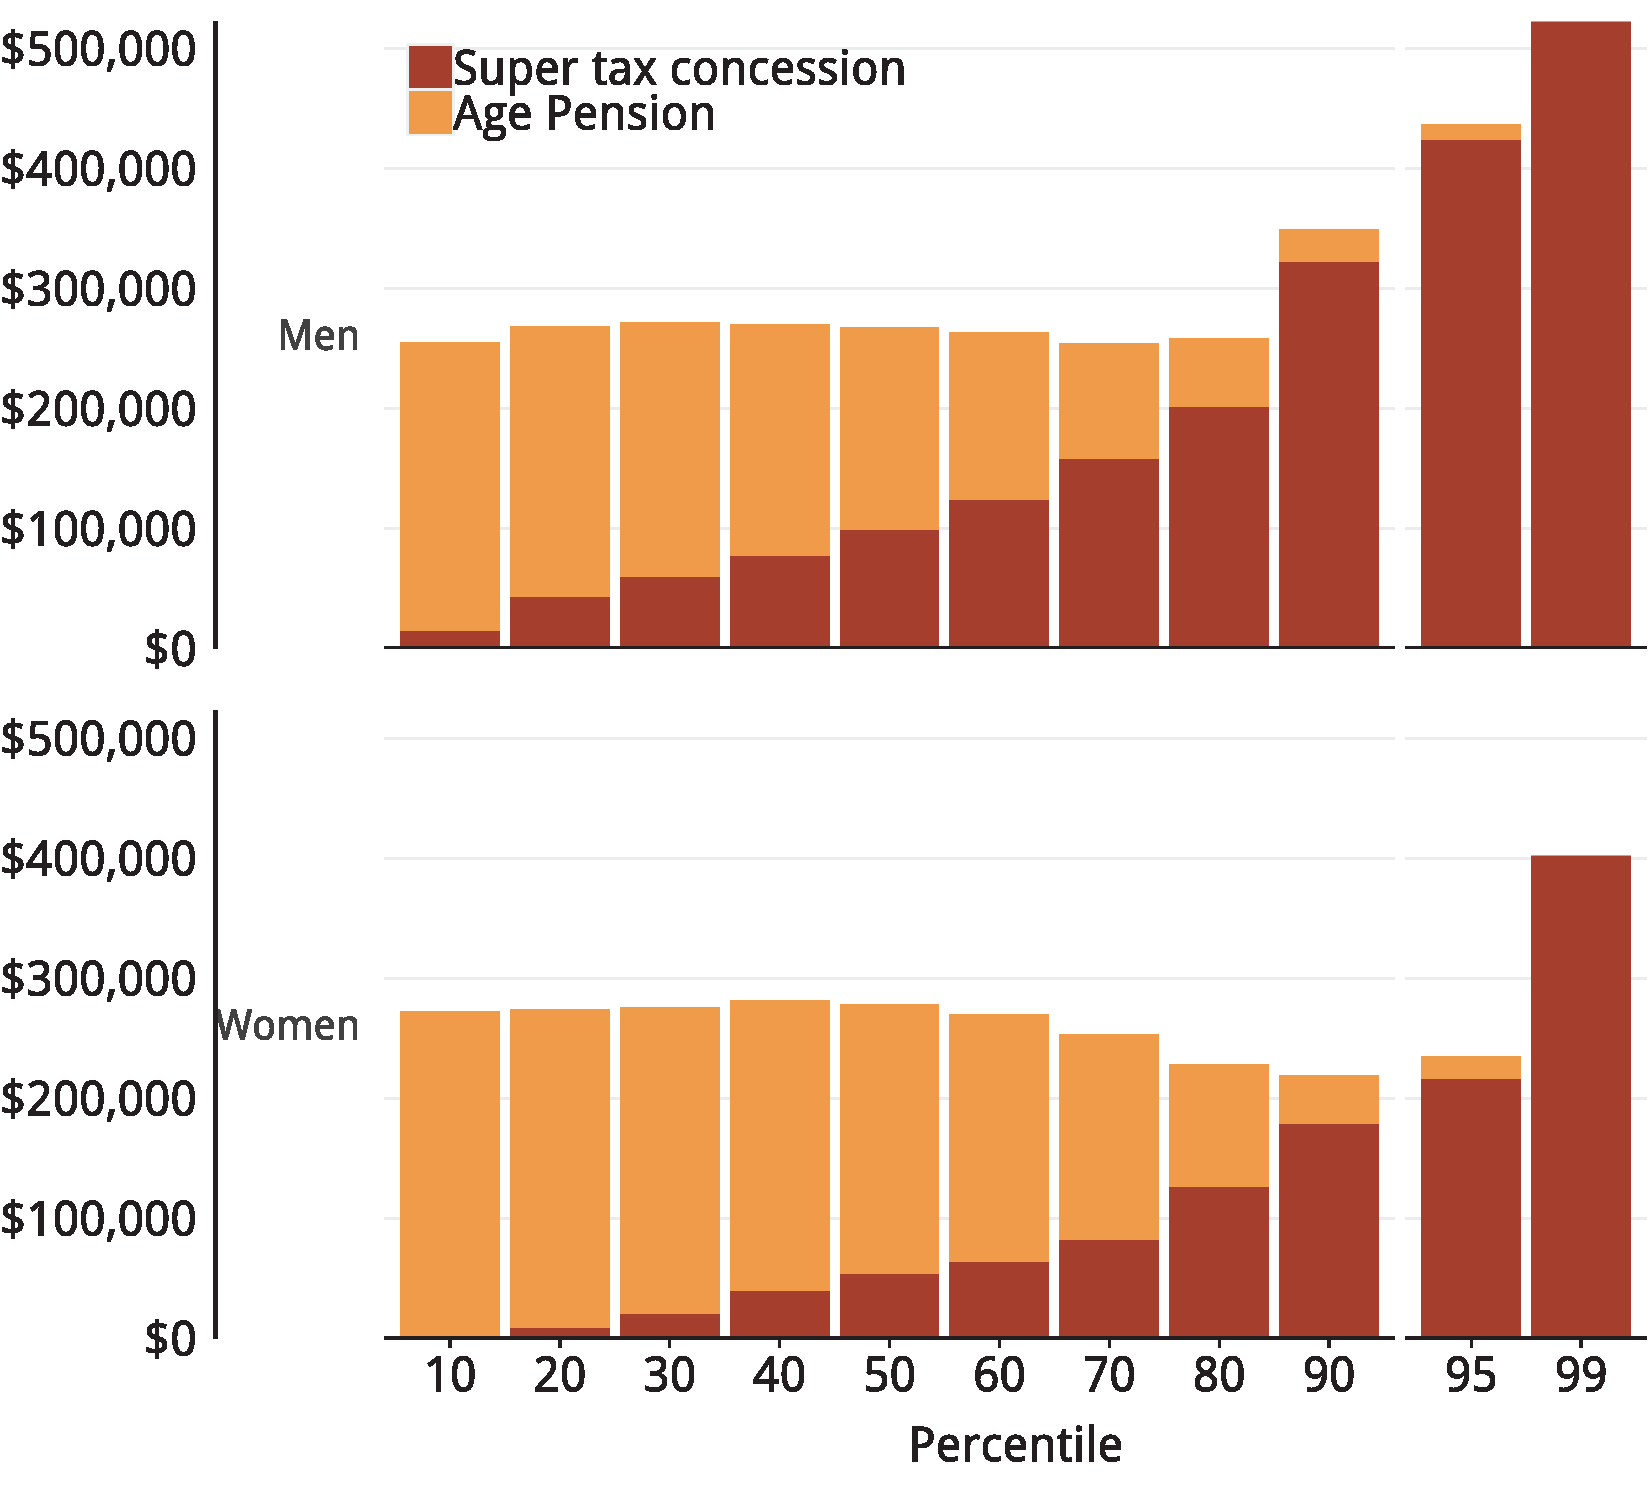
\includegraphics[width=11.000in,height=10in]{./Super-tax-targeting/b5-super-atlas/Figure3-9-1} 

\end{knitrout}

\begin{knitrout}
\definecolor{shadecolor}{rgb}{0.969, 0.969, 0.969}\color{fgcolor}
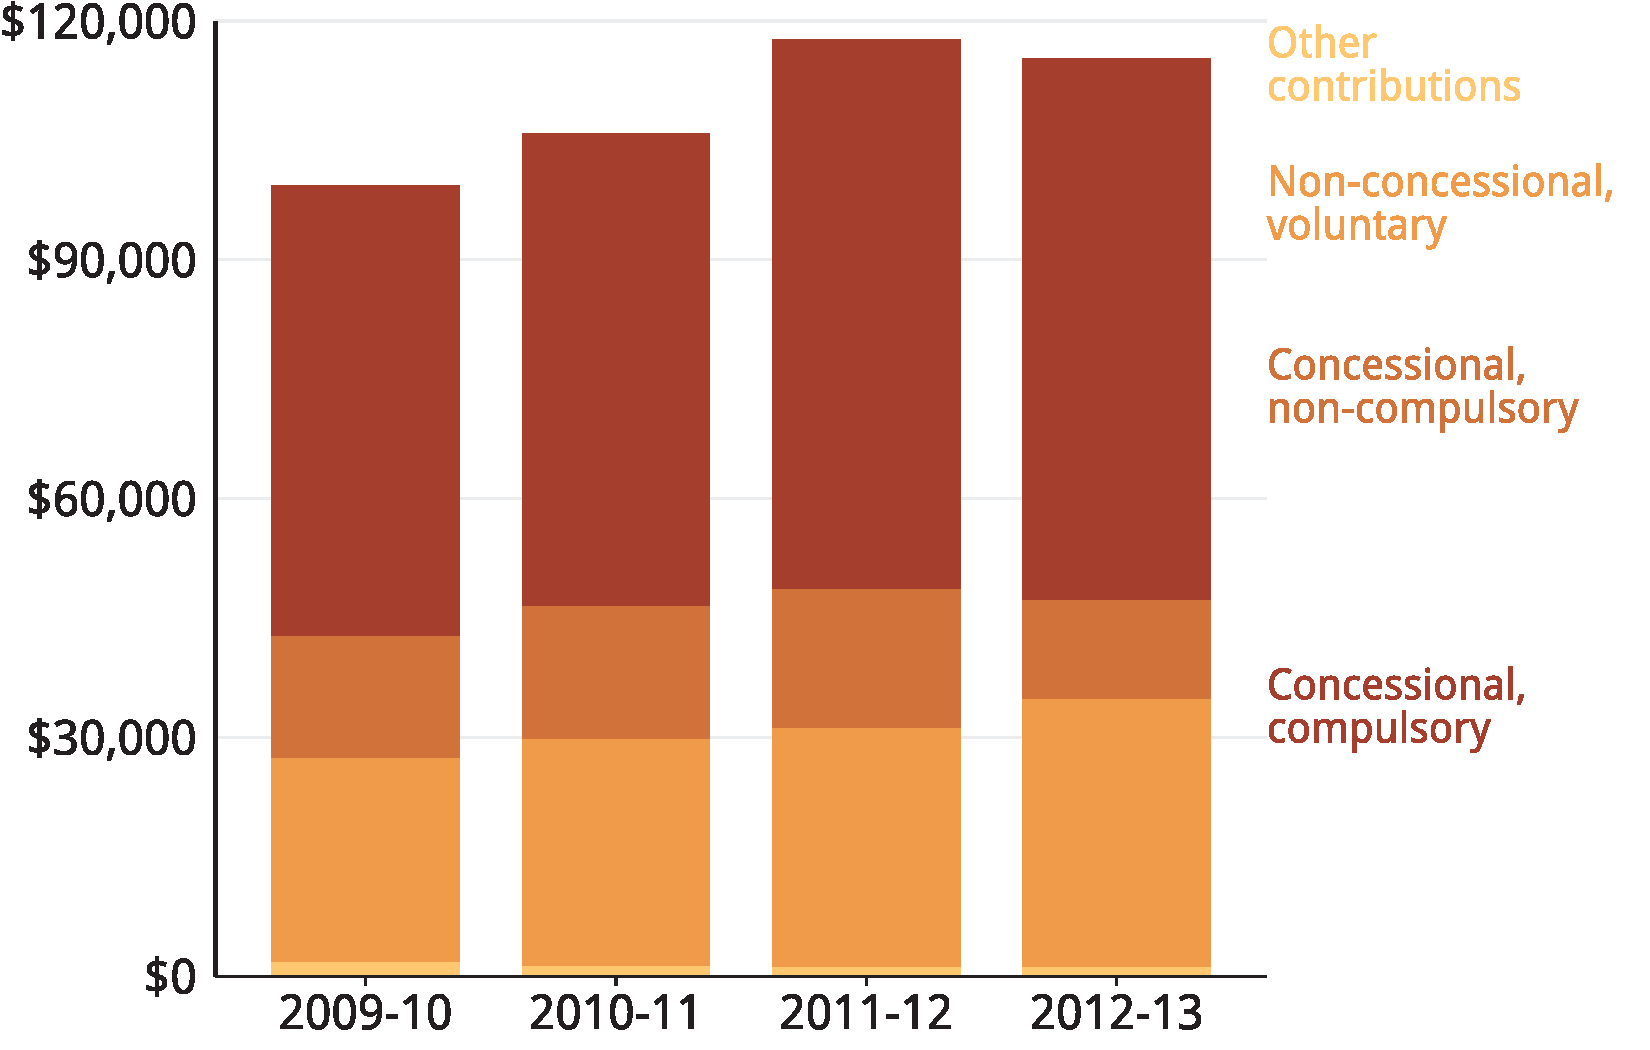
\includegraphics[width=11.000in,height=7.00in]{./Super-tax-targeting/b5-super-atlas/Figure4-1-1} 

\end{knitrout}

\begin{knitrout}
\definecolor{shadecolor}{rgb}{0.969, 0.969, 0.969}\color{fgcolor}
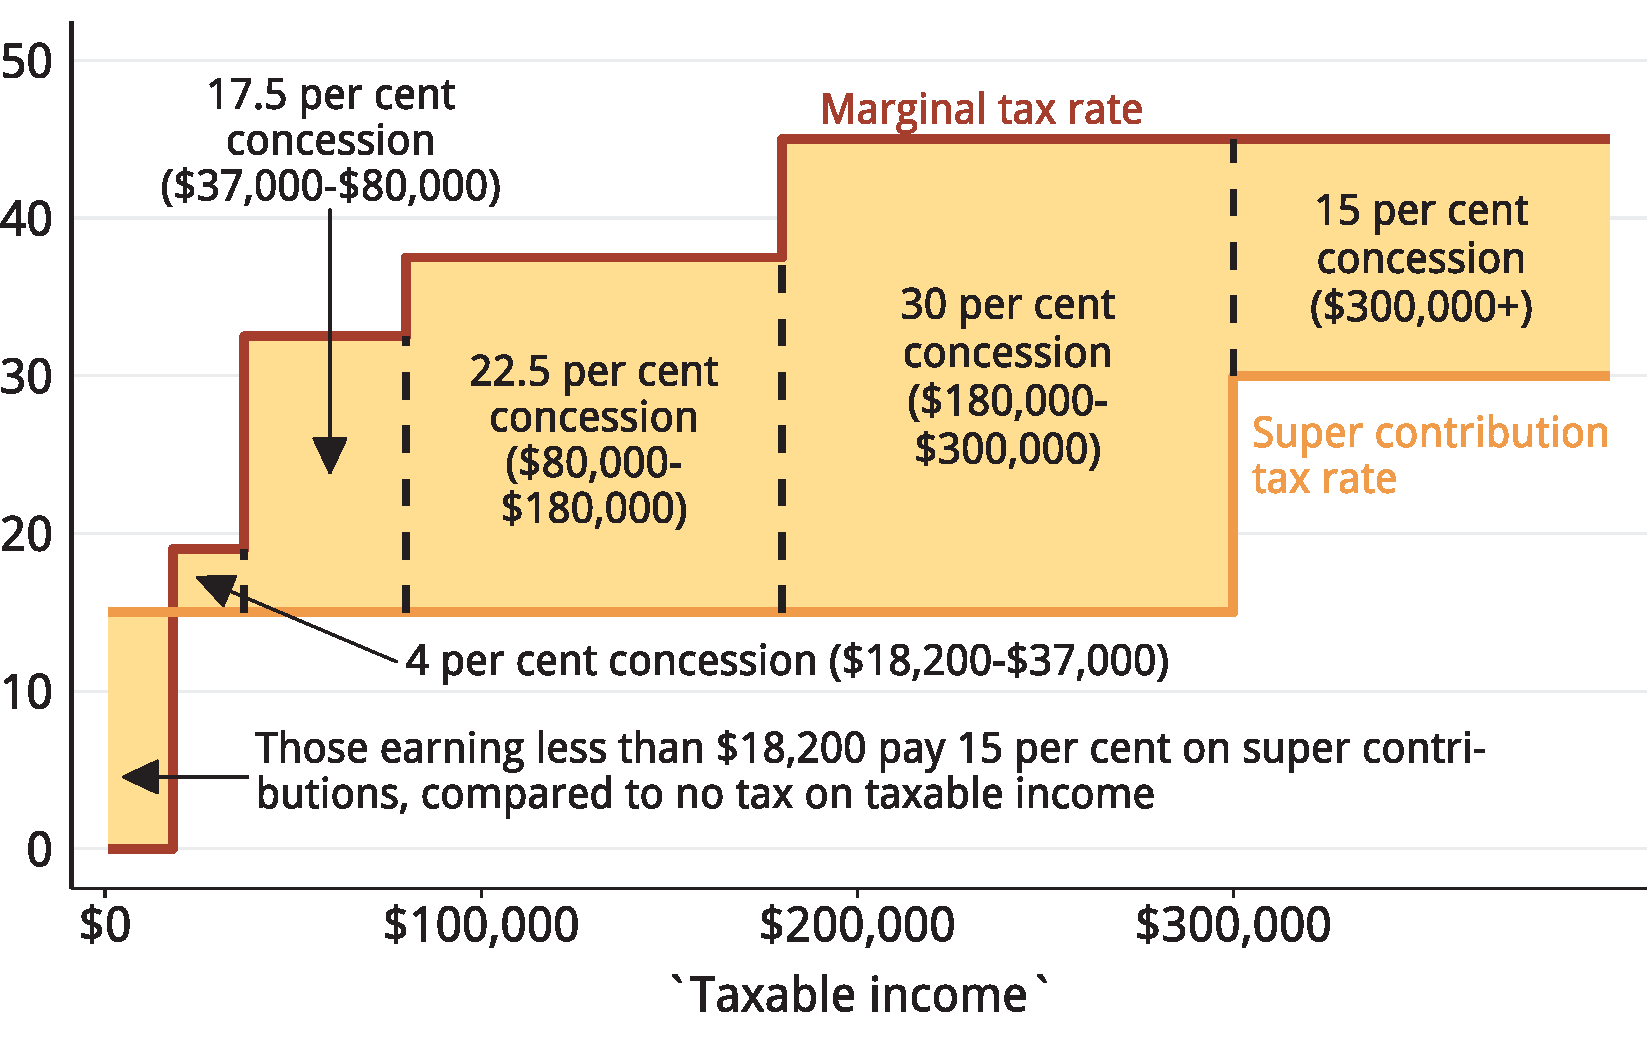
\includegraphics[width=11.000in,height=7.00in]{./Super-tax-targeting/b5-super-atlas/Figure4-2-1} 

\end{knitrout}

\begin{knitrout}
\definecolor{shadecolor}{rgb}{0.969, 0.969, 0.969}\color{fgcolor}
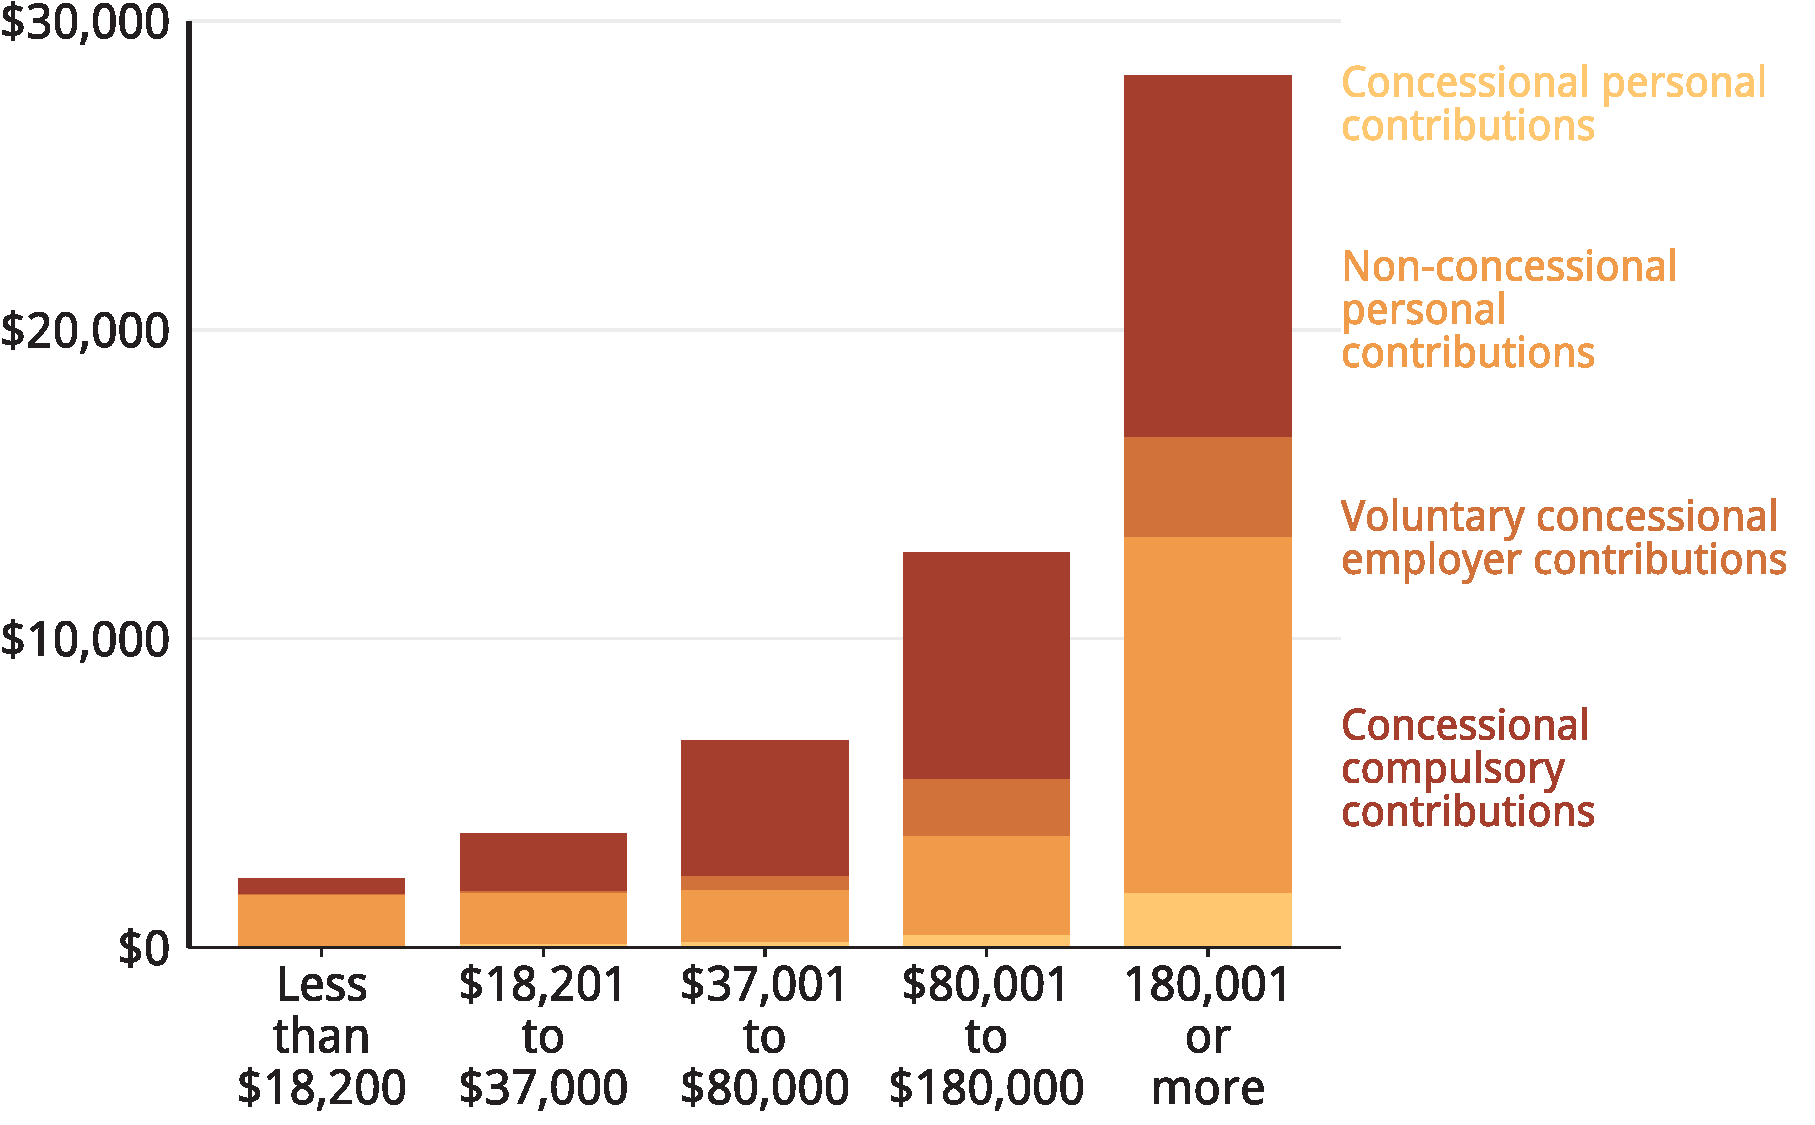
\includegraphics[width=12.1in,height=7.5in]{./Super-tax-targeting/b5-super-atlas/Figure4-3-1} 

\end{knitrout}

\begin{knitrout}
\definecolor{shadecolor}{rgb}{0.969, 0.969, 0.969}\color{fgcolor}
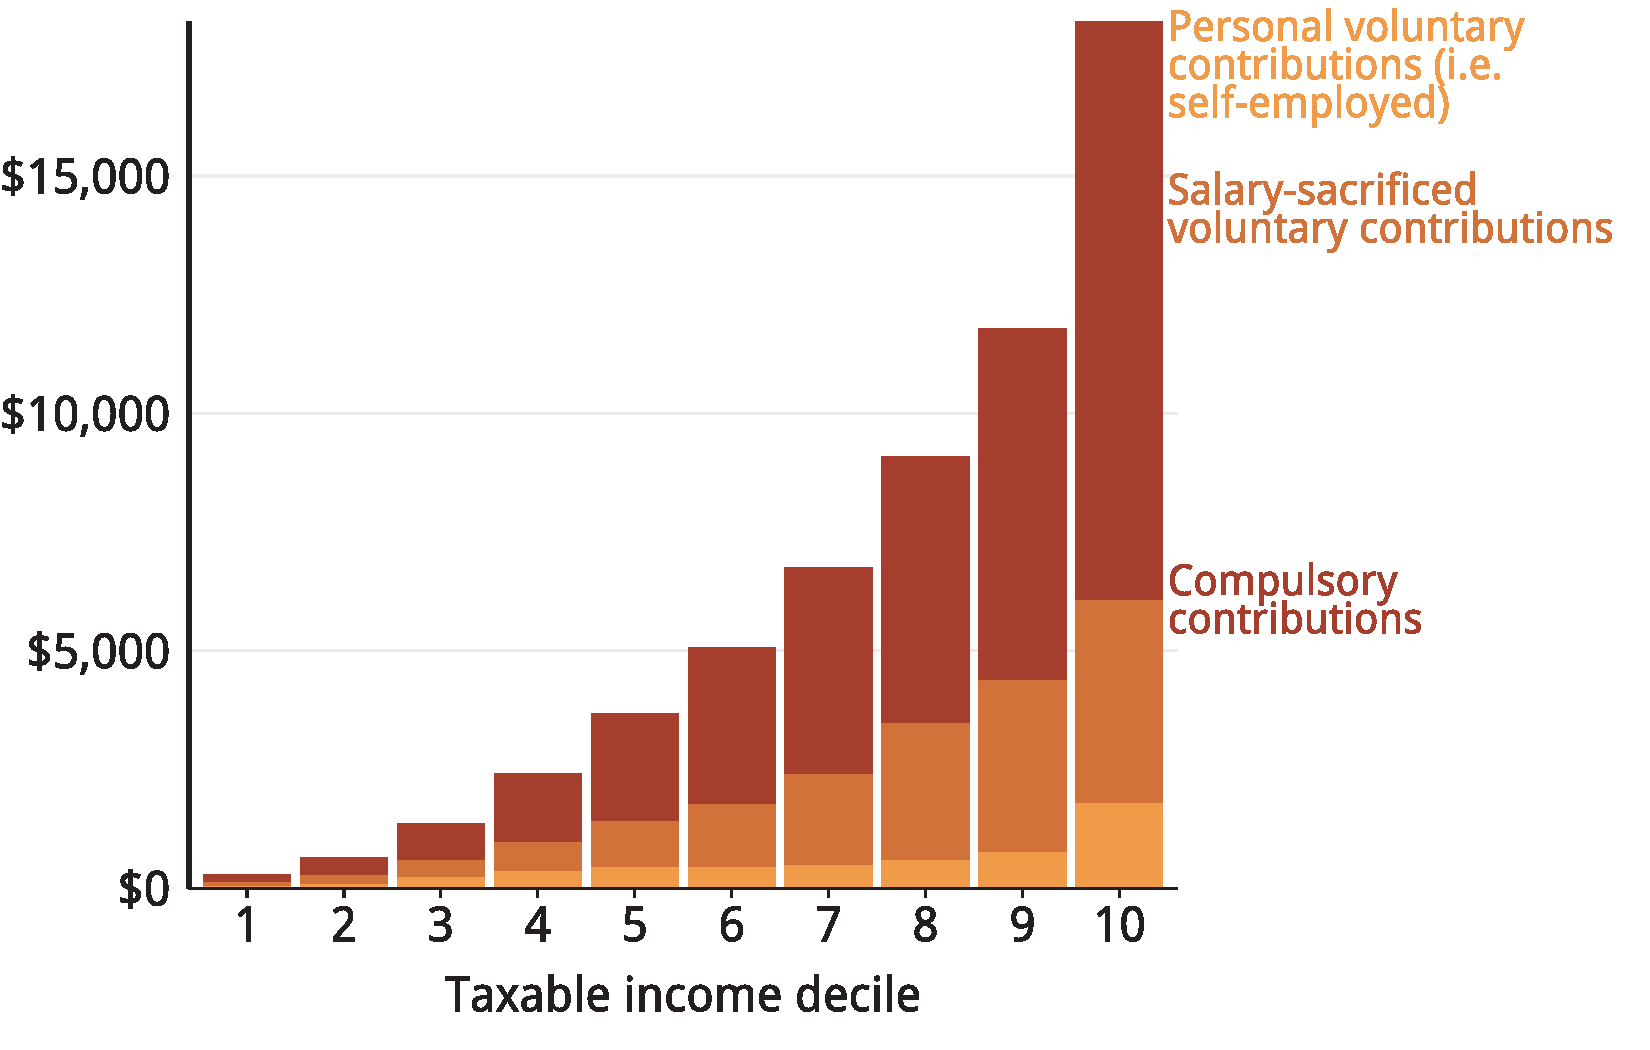
\includegraphics[width=11.000in,height=7.00in]{./Super-tax-targeting/b5-super-atlas/Figure4-4-1} 

\end{knitrout}

\begin{knitrout}
\definecolor{shadecolor}{rgb}{0.969, 0.969, 0.969}\color{fgcolor}
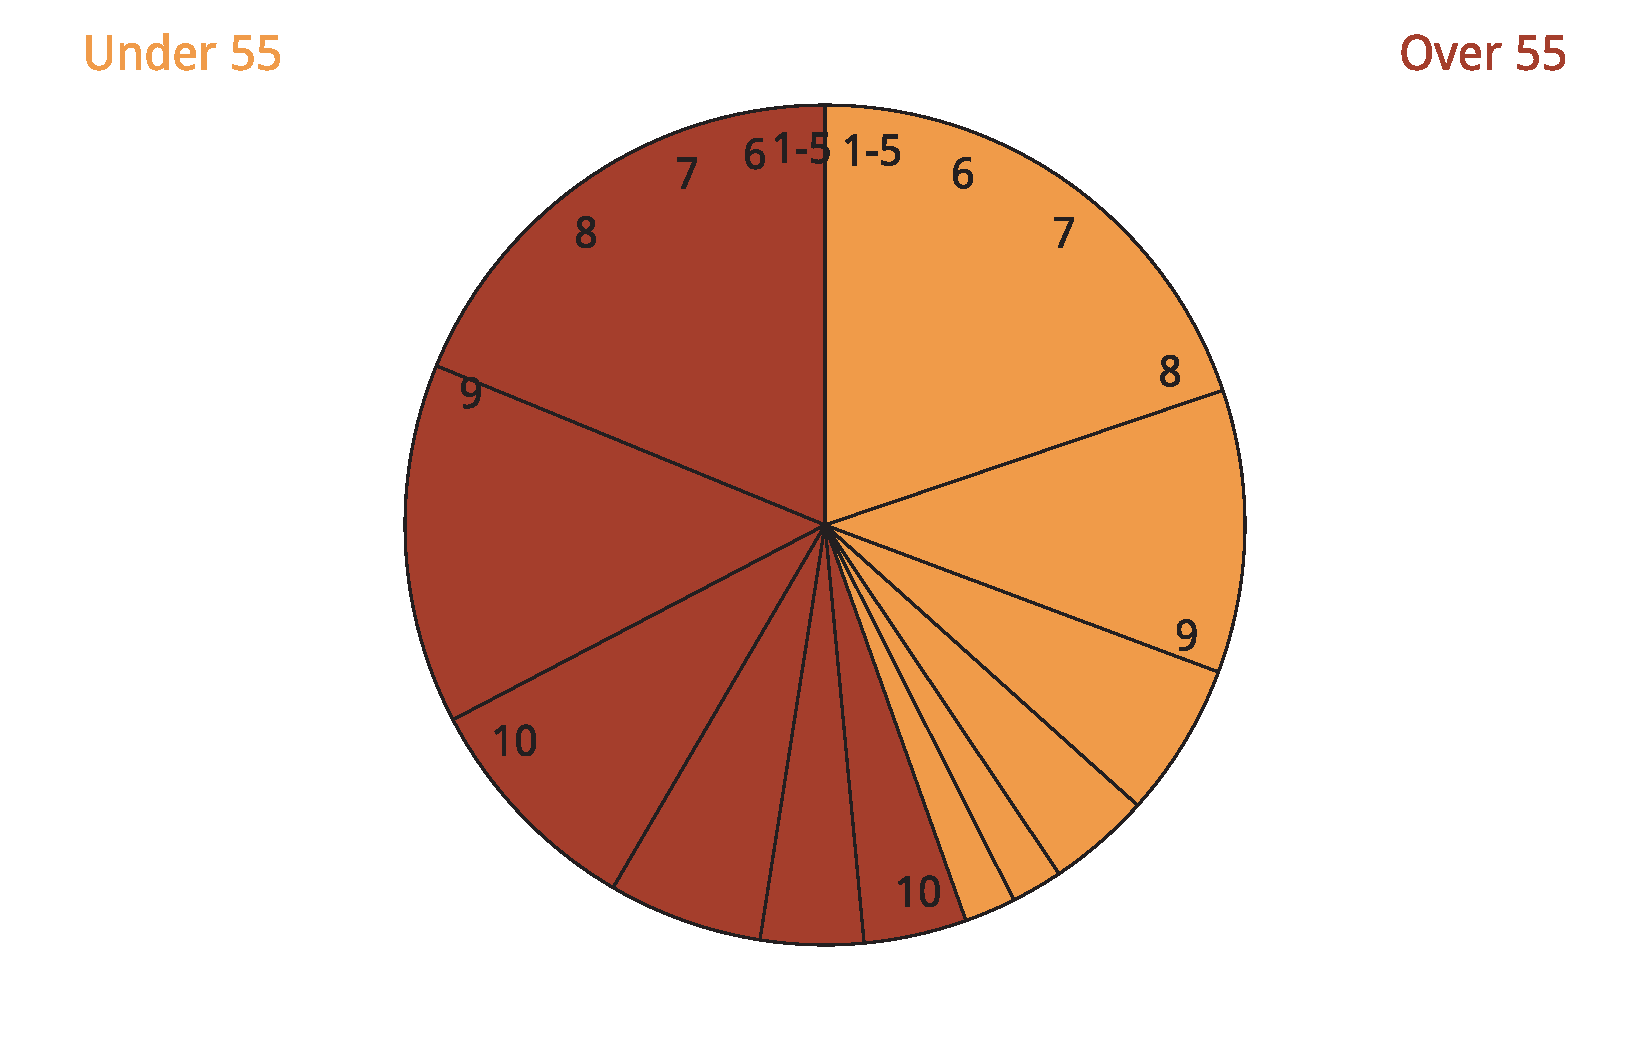
\includegraphics[width=11.000in,height=7in]{./Super-tax-targeting/b5-super-atlas/Figure4-5-1} 

\end{knitrout}

\begin{knitrout}
\definecolor{shadecolor}{rgb}{0.969, 0.969, 0.969}\color{fgcolor}
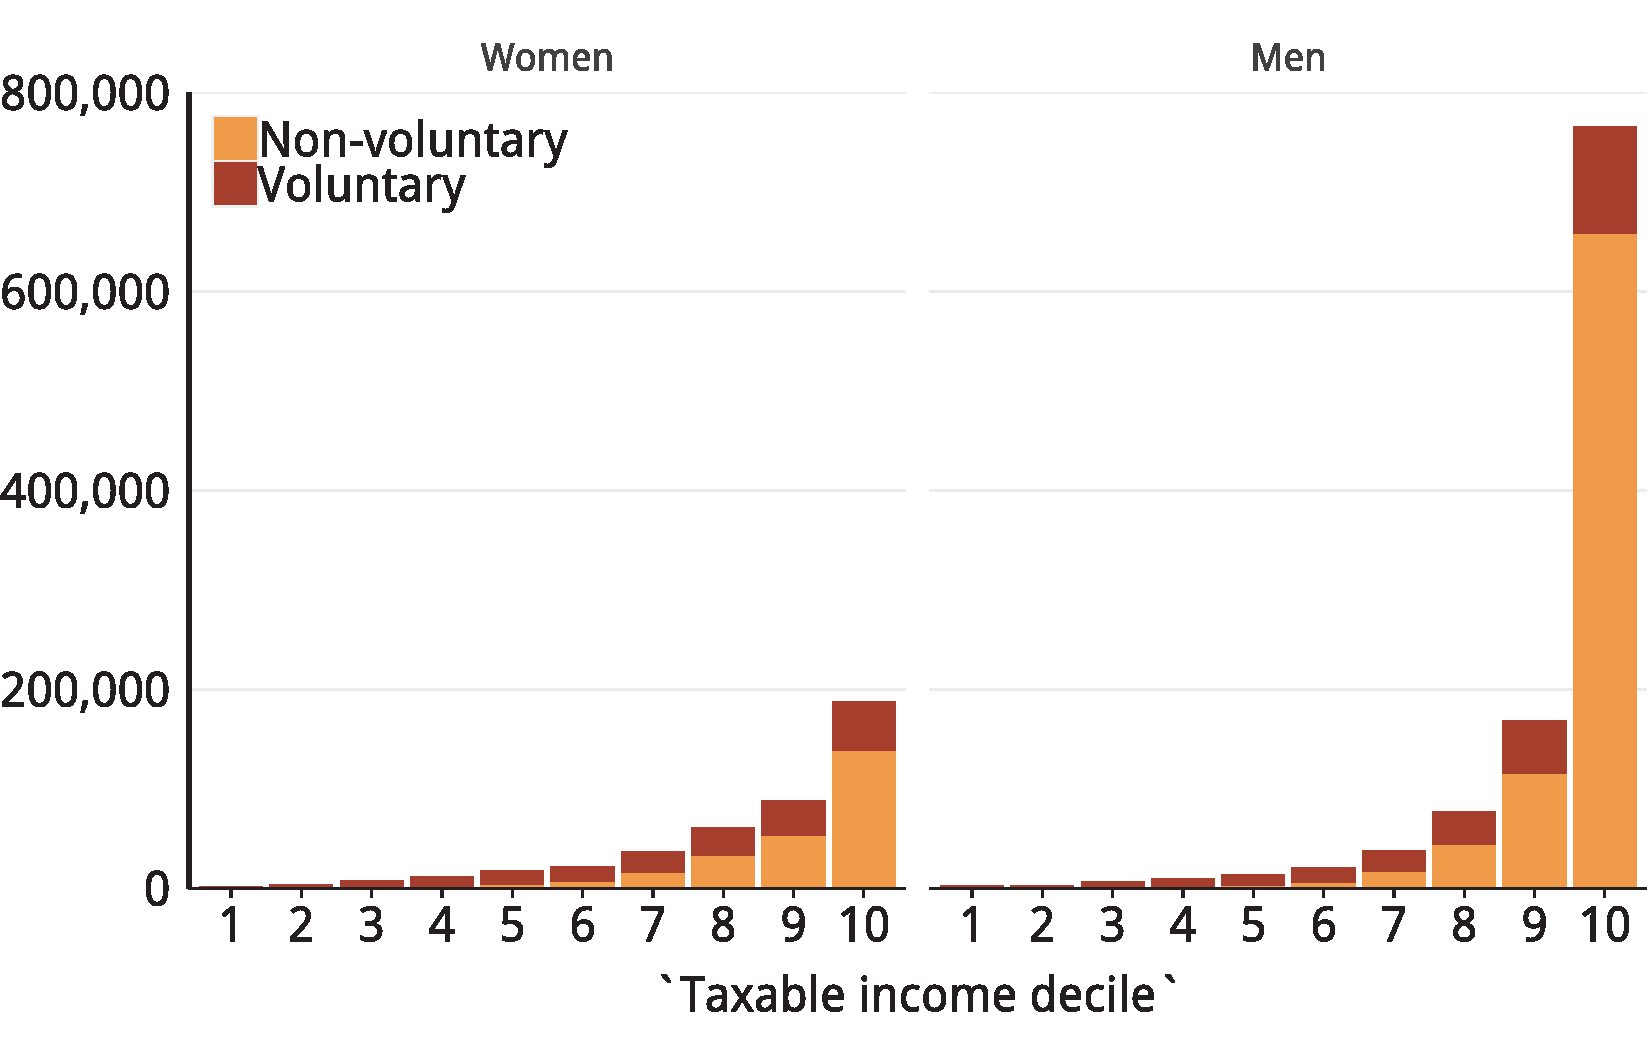
\includegraphics[width=11.000in,height=7.00in]{./Super-tax-targeting/b5-super-atlas/Figure4-6-1} 

\end{knitrout}

\begin{knitrout}
\definecolor{shadecolor}{rgb}{0.969, 0.969, 0.969}\color{fgcolor}
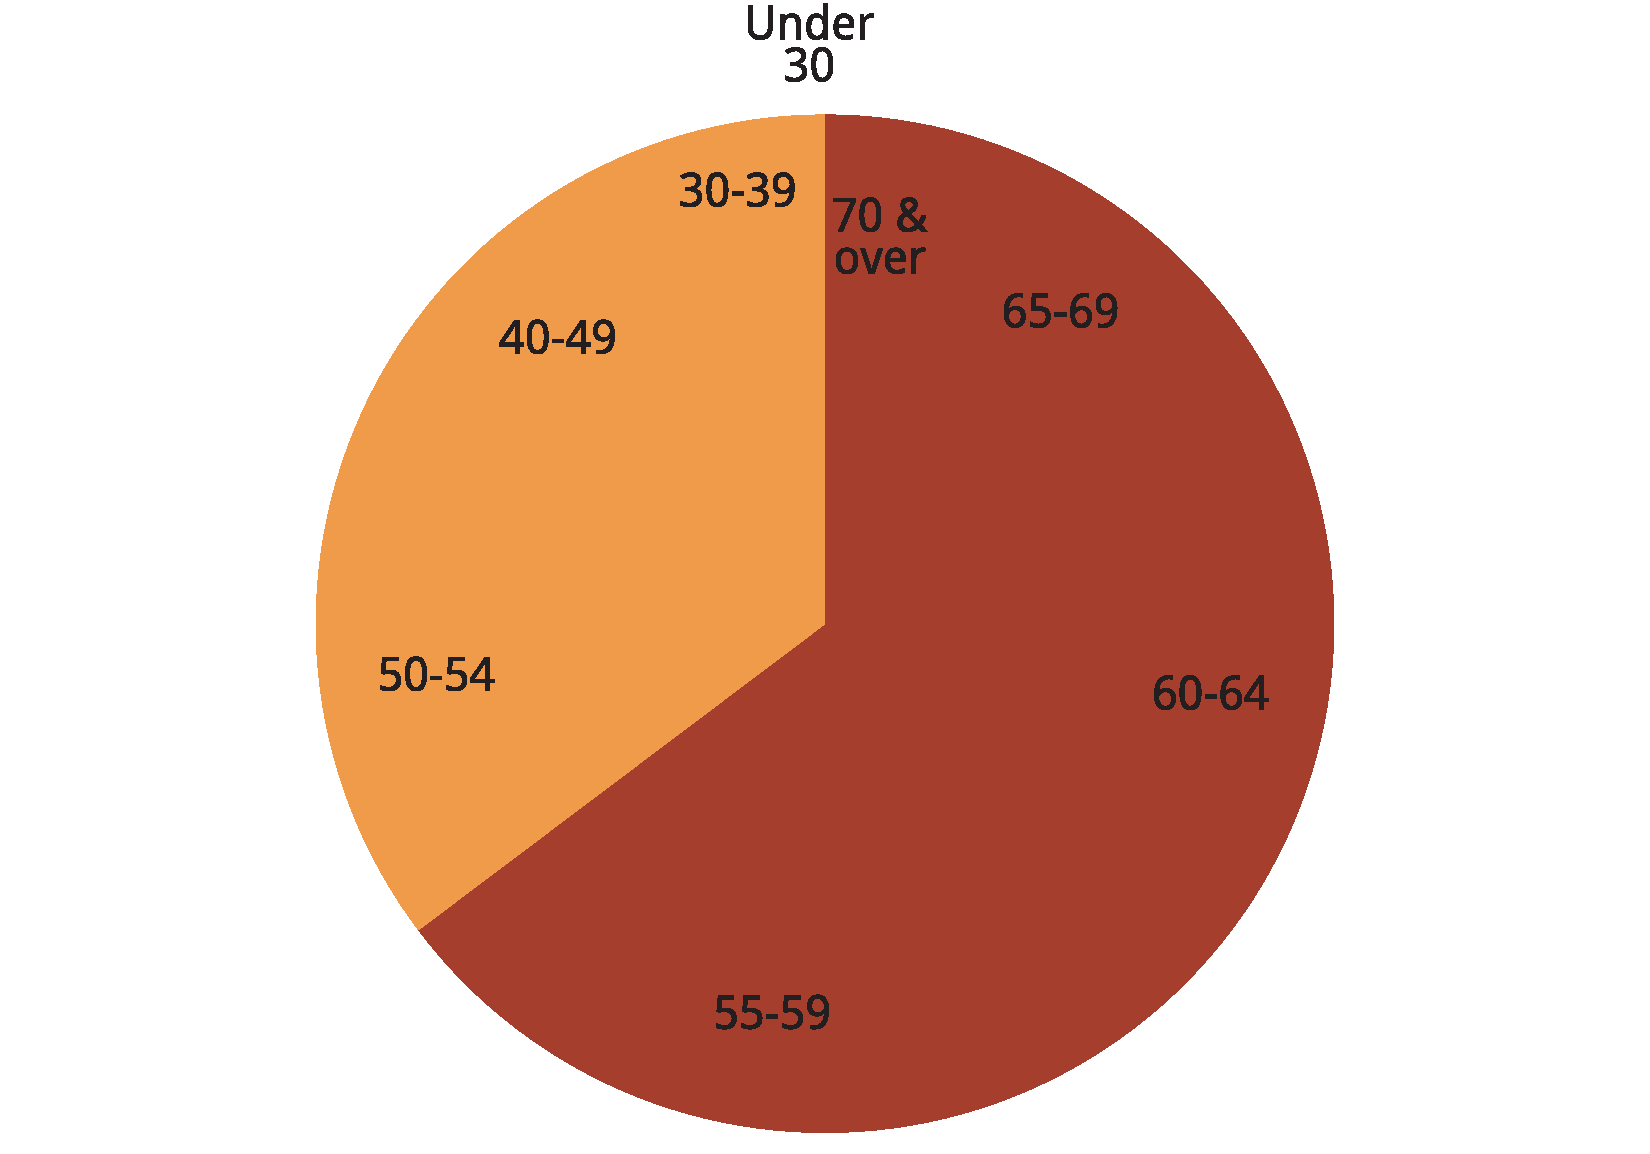
\includegraphics[width=11.000in,height=7.7in]{./Super-tax-targeting/b5-super-atlas/Figure4-7-1} 

\end{knitrout}

\begin{knitrout}
\definecolor{shadecolor}{rgb}{0.969, 0.969, 0.969}\color{fgcolor}

\includegraphics[width=11.000in,height=13in]{./Super-tax-targeting/b5-super-atlas/Figure4-8-1} 

\end{knitrout}

\begin{knitrout}
\definecolor{shadecolor}{rgb}{0.969, 0.969, 0.969}\color{fgcolor}
\includegraphics[width=11.000in,height=7.00in]{./Super-tax-targeting/b5-super-atlas/Figure4-9-1} 

\end{knitrout}

\begin{knitrout}
\definecolor{shadecolor}{rgb}{0.969, 0.969, 0.969}\color{fgcolor}
\includegraphics[width=11.000in,height=8in]{./Super-tax-targeting/b5-super-atlas/Figure4-10-1} 

\end{knitrout}


%% Here!
\begin{knitrout}
\definecolor{shadecolor}{rgb}{0.969, 0.969, 0.969}\color{fgcolor}
\includegraphics[width=11.000in,height=7.00in]{./Super-tax-targeting/b5-super-atlas/Figure5-1-1} 

\end{knitrout}

\begin{knitrout}
\definecolor{shadecolor}{rgb}{0.969, 0.969, 0.969}\color{fgcolor}
\includegraphics[width=12.1in,height=7.00in]{./Super-tax-targeting/b5-super-atlas/Figure5-2-1} 

\end{knitrout}

\begin{knitrout}
\definecolor{shadecolor}{rgb}{0.969, 0.969, 0.969}\color{fgcolor}
\includegraphics[width=11.000in,height=7.00in]{./Super-tax-targeting/b5-super-atlas/Figure6-1-1} 

\end{knitrout}

\begin{knitrout}
\definecolor{shadecolor}{rgb}{0.969, 0.969, 0.969}\color{fgcolor}
\includegraphics[width=11.000in,height=7.00in]{./Super-tax-targeting/b5-super-atlas/Figure6-2-orig-1} 

\end{knitrout}

\begin{knitrout}
\definecolor{shadecolor}{rgb}{0.969, 0.969, 0.969}\color{fgcolor}
\includegraphics[width=11.000in,height=13in]{./Super-tax-targeting/b5-super-atlas/Figure6-2-1} 

\end{knitrout}

\begin{knitrout}
\definecolor{shadecolor}{rgb}{0.969, 0.969, 0.969}\color{fgcolor}
\includegraphics[width=13.2in,height=7in]{./Super-tax-targeting/b5-super-atlas/Figure6-3-1} 

\end{knitrout}

\begin{knitrout}
\definecolor{shadecolor}{rgb}{0.969, 0.969, 0.969}\color{fgcolor}\begin{kframe}


{\ttfamily\noindent\bfseries\color{errorcolor}{\#\# Error: `path` does not exist: './Super-tax-targeting/super-atlas/appendices/Figure-A-1.xlsx'}}

{\ttfamily\noindent\bfseries\color{errorcolor}{\#\# Error in eval(lhs, parent, parent): object 'a1' not found}}\end{kframe}
\end{knitrout}
\begin{knitrout}
\definecolor{shadecolor}{rgb}{0.969, 0.969, 0.969}\color{fgcolor}\begin{kframe}


{\ttfamily\noindent\bfseries\color{errorcolor}{\#\# Error in eval(lhs, parent, parent): object 'a1' not found}}\end{kframe}
\end{knitrout}

\section{CGT}



\begin{knitrout}
\definecolor{shadecolor}{rgb}{0.969, 0.969, 0.969}\color{fgcolor}\begin{kframe}


{\ttfamily\noindent\bfseries\color{errorcolor}{\#\# Error in eval(expr, envir, enclos): object 'sample\_files\_all' not found}}\end{kframe}
\end{knitrout}

\begin{knitrout}
\definecolor{shadecolor}{rgb}{0.969, 0.969, 0.969}\color{fgcolor}\begin{kframe}


{\ttfamily\noindent\bfseries\color{errorcolor}{\#\# Error in merge(sample\_file, age\_range\_decoder, by = "{}age\_range"{}): object 'sample\_file' not found}}

{\ttfamily\noindent\bfseries\color{errorcolor}{\#\# Error in eval(lhs, parent, parent): object 'sample\_file' not found}}\end{kframe}
\end{knitrout}

\begin{knitrout}
\definecolor{shadecolor}{rgb}{0.969, 0.969, 0.969}\color{fgcolor}
\includegraphics[width=11.000in,height=7.00in]{./Hot-property-CG-and-NG/CGT-NG-atlas/b5-atlas/CGT-Figure1-1} 

\end{knitrout}

\begin{knitrout}
\definecolor{shadecolor}{rgb}{0.969, 0.969, 0.969}\color{fgcolor}\begin{kframe}


{\ttfamily\noindent\bfseries\color{errorcolor}{\#\# Error in eval(lhs, parent, parent): object 'sample\_file' not found}}\end{kframe}
\end{knitrout}
\clearpage


\section{cgt}


\subsection{Individuals earn most capital gains through real estate and shares}
\begin{knitrout}
\definecolor{shadecolor}{rgb}{0.969, 0.969, 0.969}\color{fgcolor}
\includegraphics[width=11.000in,height=7.00in]{./Hot-property-CG-and-NG/CGT-NG-atlas/b5-palatino-atlas/CGT-by-asset-1} 

\end{knitrout}

\begin{knitrout}
\definecolor{shadecolor}{rgb}{0.969, 0.969, 0.969}\color{fgcolor}
\includegraphics[width=11.000in,height=8in]{./Hot-property-CG-and-NG/CGT-NG-atlas/b5-palatino-atlas/CG-marginal-tax-rates-delayed-1} 

\end{knitrout}

\begin{knitrout}
\definecolor{shadecolor}{rgb}{0.969, 0.969, 0.969}\color{fgcolor}\begin{kframe}


{\ttfamily\noindent\bfseries\color{errorcolor}{\#\# Error in mutate\_impl(.data, dots): Evaluation error: `to\_fy` is missing, with no default..}}\end{kframe}
\end{knitrout}


\begin{knitrout}
\definecolor{shadecolor}{rgb}{0.969, 0.969, 0.969}\color{fgcolor}
\includegraphics[width=11.000in,height=7.00in]{./Hot-property-CG-and-NG/CGT-NG-atlas/b5-palatino-atlas/CGT-fig16-1} 

\end{knitrout}

\subsection{Rents did not rise when negative gearing was removed in Melbourne\dots}
\begin{knitrout}
\definecolor{shadecolor}{rgb}{0.969, 0.969, 0.969}\color{fgcolor}\begin{kframe}


{\ttfamily\noindent\bfseries\color{errorcolor}{\#\# Error in gzfile(file, "{}rb"{}): cannot open the connection}}

{\ttfamily\noindent\bfseries\color{errorcolor}{\#\# Error in eval(lhs, parent, parent): object 'rent.indices.real' not found}}\end{kframe}
\end{knitrout}

\subsection{Those earning more claim bigger primary production losses}
\begin{knitrout}
\definecolor{shadecolor}{rgb}{0.969, 0.969, 0.969}\color{fgcolor}
\includegraphics[width=13.2in,height=7.00in]{./Hot-property-CG-and-NG/CGT-NG-atlas/b5-palatino-atlas/PP-losers-salary-comparison-horiz-bar-1} 

\end{knitrout}

\begin{knitrout}
\definecolor{shadecolor}{rgb}{0.969, 0.969, 0.969}\color{fgcolor}
\includegraphics[width=8.8in,height=7.00in]{./Hot-property-CG-and-NG/CGT-NG-atlas/b5-palatino-atlas/Proportions-PP-losses-1} 

\end{knitrout}





\end{document}
